% MosaicOpt paper - SIGMOD double-blind draft
% Compile with: pdflatex paper.tex (twice), bibtex paper, pdflatex paper.tex (twice)

\documentclass[sigconf,nonacm,review]{acmart}

% ---------- Packages ----------
\usepackage{amsmath}
% amssymb intentionally omitted: newtxmath (loaded by acmart) already
% provides the AMS symbol set, and the two packages collide on \Bbbk.
\usepackage{amsthm}
\usepackage{mathrsfs}
\usepackage{booktabs}
\usepackage{multirow}
\usepackage{array}
\usepackage{xcolor}
\usepackage{tikz}
\usetikzlibrary{positioning, arrows.meta, calc, shapes, fit, backgrounds, shadows.blur, decorations.pathreplacing, decorations.pathmorphing}
\usepackage[utf8]{inputenc}
\usepackage[T1]{fontenc}
\usepackage{microtype}
\usepackage{enumitem}
\usepackage{listings}
\usepackage{xspace}
\usepackage{algorithm}
\usepackage{algpseudocode}

% ---------- Color palette (matches presentation) ----------
\definecolor{mosaicCrimson}{HTML}{780000}
\definecolor{mosaicBlue}{HTML}{003049}
\definecolor{mosaicLightBlue}{HTML}{669BBC}
\definecolor{mosaicCream}{HTML}{FDF0D5}
\definecolor{mosaicRed}{HTML}{C1121F}
\definecolor{mosaicGray}{HTML}{8D99AE}

% ---------- Listings (SQL code blocks in Section 5) ----------
\lstset{
  basicstyle=\ttfamily\small,
  keywordstyle=\color{mosaicBlue}\bfseries,
  commentstyle=\color{mosaicGray}\itshape,
  stringstyle=\color{mosaicCrimson},
  showstringspaces=false,
  breaklines=true,
  breakatwhitespace=true,
  columns=fullflexible,
  keepspaces=true,
  numbers=none,
  frame=single,
  rulecolor=\color{mosaicLightBlue},
  framesep=4pt,
  xleftmargin=2pt,
  xrightmargin=2pt,
  aboveskip=8pt,
  belowskip=8pt,
  language=SQL
}

% ---------- Theorem-like environments ----------
\theoremstyle{plain}
\newtheorem{theorem}{Theorem}
\newtheorem{lemma}[theorem]{Lemma}
\newtheorem{corollary}[theorem]{Corollary}
\newtheorem{proposition}[theorem]{Proposition}

\theoremstyle{definition}
\newtheorem{definition}{Definition}

\newtheorem{counterexample}{Counterexample}

% Proof is built-in; redefine QED
\renewcommand{\qedsymbol}{\ensuremath{\blacksquare}}

% ---------- Notation shortcuts ----------
\newcommand{\vect}[1]{\boldsymbol{#1}}
\newcommand{\attr}[1]{\operatorname{attr}(#1)}
\newcommand{\Mem}{\mathit{Mem}}
\newcommand{\KG}{\mathit{KG}}
\newcommand{\schema}[1]{\operatorname{schema}(#1)}
\newcommand{\setof}[1]{\operatorname{set}(#1)}
\newcommand{\topK}{\operatorname{topK}}
\newcommand{\bm}[1]{\boldsymbol{#1}}

% Remark environment (used for non-blocking observations)
\theoremstyle{remark}
\newtheorem{remark}{Remark}

% ---------- CCS / Metadata ----------
\acmConference[SIGMOD '25]{ACM SIGMOD International Conference on Management of Data}{2025}{}
\setcopyright{none}

\begin{CCSXML}
<ccs2012>
<concept>
<concept_id>10002951.10003317.10003331</concept_id>
<concept_desc>Information systems~Database management system engines</concept_desc>
<concept_significance>500</concept_significance>
</concept>
<concept>
<concept_id>10002951.10003317.10003338</concept_id>
<concept_desc>Information systems~Query optimization</concept_desc>
<concept_significance>500</concept_significance>
</concept>
<concept>
<concept_id>10002951.10003317.10003332</concept_id>
<concept_desc>Information systems~Database design and models</concept_desc>
<concept_significance>300</concept_significance>
</concept>
</ccs2012>
\end{CCSXML}

\keywords{agentic memory, relational algebra, query optimization, vector search, hybrid retrieval, rule-based optimizer, equational theory}

% =====================================================================
% Title
% =====================================================================
\title{MosaicOpt: An Algebraic Foundation for Agentic Memory Databases}

\author{Anonymous Author(s)}
\affiliation{
  \institution{Anonymous Institution}
  \city{Anonymous City}
  \state{Anonymous State}
  \country{Anonymous Country}}
\email{anonymous@example.com}

\begin{document}
\begin{abstract}
\noindent
Production LLM agents accumulate multi-modal memory across two timescales:
long-term facts and preferences, and short-term working context. A memory
unit typically carries text, one or more dense vector embeddings,
structured metadata, and graph relations. Useful queries against this
store are conjunctive expressions that mix all four modalities --- for
example, ``find passages about a fault-tolerance bug from the last 30
days, semantically similar to a stack trace, attributed to a known
subsystem, and connected by a derivation link to a prior incident.'' The
dominant engineering response, \emph{multi-path recall} with
application-level score fusion, has no principled semantics, no
equivalence relation over plans, and breaks down on multi-vector
conjunctions. We propose \textbf{MosaicOpt}, an \emph{algebra-first}
design that extends relational algebra with (i) a \emph{materialization}
operator $\mu$ that binds computed values (vector distances, BM25
scores) as first-class attributes, (ii) first-class vector, text, and
graph predicates, and (iii) a graph expansion operator $\Gamma$. The
optimizer is a Volcano/Cascades-style rule-based layer driven by an
\emph{equational theory} of seven foundational identities (M1--M5,
G1, G2) over the extended operators, supplemented by the assumed
classical A1--A8 (including join commutativity and associativity; A1
and A4 apply naturally to vector predicates), the derived chains
(M4+M1, M5+G1, A4-vector+M1), the classical applications
(A7-symmetry, A8-regrouping), the definitional
$\tau$-$\Lambda$-$\topK$ rewrite, and the row-preserving
$\sigma$-$\tau$ commutation, combined with a cost-based layer that
explicitly accounts for approximation. We prove the identities, give counterexamples for the
non-identities (N1--N5) that classical intuition suggests but
approximation, graph-traversal asymmetry, or the
traversal-vs-origin column split break, and sketch a prototype and
evaluation plan. The argument is foundational: agentic memory is a
query problem, query
problems benefit from algebraic foundations, and an extension of
relational algebra is the natural place to start.
\end{abstract}

\maketitle

% =====================================================================
% 1. Introduction & Motivation
% =====================================================================
\section{Introduction \& Motivation}\label{sec:intro}

Large language model (LLM) agents are no longer stateless
request--response loops. Production agents --- coding copilots, personal
assistants, autonomous research workers, multi-step planners ---
accumulate state across two timescales: \emph{long-term memory}, which
persists facts, preferences, and episodic traces across sessions; and
\emph{short-term memory}, which captures the working context of an
in-flight session, including tool-call history and intermediate
reasoning artifacts. This split is widely accepted in the
agentic-systems literature, but its consequences for the storage layer
have received less attention.

The content of agentic memory is \emph{multi-modal}. A
single ``memory unit'' may carry: (i)~raw text (a chat snippet, a code
diff, a document excerpt); (ii)~one or more dense vector embeddings,
often produced by different encoders for different retrieval objectives
(e.g. semantic similarity, intent classification, code search);
(iii)~structured metadata (timestamps, source, provenance, user tags,
confidence scores); and (iv)~graph structure (entity relations such as
\texttt{derived\_from}, \texttt{cites}, \texttt{contradicts},
\texttt{member\_of}). A useful query against this store is seldom a pure
similarity lookup; it is a \emph{conjunctive} expression that mixes all
four modalities. ``Find passages about a fault tolerance bug from the
last 30 days, semantically similar to this stack trace, attributed to a
known subsystem, and connected by \texttt{derived\_from} to a previous
incident'' is representative.

The dominant engineering response is \emph{multi-path recall}: a
fan-out across specialized engines (a vector index, a full-text index,
a key--value store, a graph store), each producing a ranked candidate
list, followed by application-level score fusion and re-ranking.
Frameworks such as Mem0 \cite{mem0}, Letta \cite{letta}, Zep, and
Cognee instantiate variations
of this pattern. It works, and there is no shortage of impressive
product demonstrations. But the pattern has four structural weaknesses:

\begin{enumerate}[leftmargin=*]
  \item \textbf{No principled semantics.} The semantics of a fused
    query is defined by the application code that combines the
    per-channel scores. Two implementations of ``find similar memory''
    in the same product can have silently different meanings.
  \item \textbf{Heuristic optimization only.} Without an algebra, there
    is no equivalence relation over plans. The ``optimizer'' is a
    hand-tuned orchestration pipeline whose rewrites are not derived
    from a sound theory.
  \item \textbf{Fusion policy leaks into the substrate.} Score
    combination functions (e.g. weighted sum, reciprocal-rank fusion,
    learned rerankers) are application concerns; once baked into a
    query template, they are hard to change without re-engineering the
    data path.
  \item \textbf{Top-$k$ per column breaks conjunctive intent.} Each
    vector column is typically searched independently with its own
    top-$k$, then intersected. For multi-vector memories, the
    intersection of per-column top-$k$ sets is frequently empty or
    impoverished, because the columns are correlated, not redundant.
\end{enumerate}

Our position is that these problems are not implementation details;
they are symptoms of a missing foundation. \textbf{MosaicOpt} proposes
an \emph{algebra-first} design in which relational algebra is extended
with a small set of operators that make multi-modal memory queries
first-class, and in which the resulting algebra --- not application
code --- is the substrate contract between query and execution. The
optimizer becomes a \emph{rule-based} layer driven by an equational
theory (Section~\ref{sec:equational}), with a
\emph{cost-based} layer (Section~\ref{sec:cbo}) choosing between
physical realizations that may legitimately differ in approximation
behaviour.

\begin{figure}[t]
  \centering
  \resizebox{\columnwidth}{!}{%
  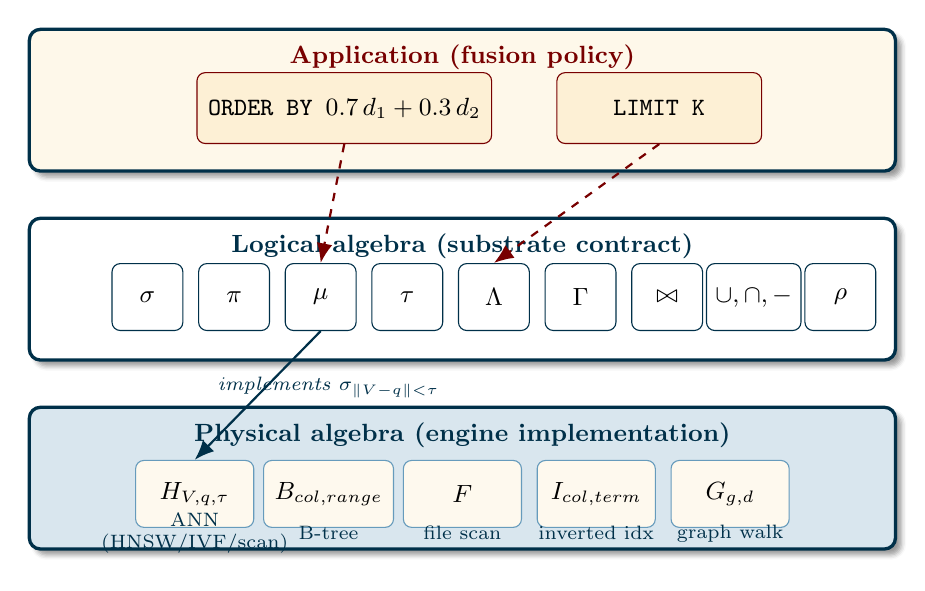
\begin{tikzpicture}[
    layer/.style={rectangle, rounded corners=4pt, draw=mosaicBlue, very thick, minimum width=11cm, minimum height=1.8cm, blur shadow={shadow blur steps=4}},
    appbox/.style={rectangle, draw=mosaicCrimson, fill=mosaicCream, rounded corners=3pt, minimum height=0.9cm, minimum width=2.6cm, font=\ttfamily\small, inner sep=4pt},
    logbox/.style={rectangle, draw=mosaicBlue, fill=white, rounded corners=3pt, minimum height=0.85cm, minimum width=0.9cm, font=\small, inner sep=2pt},
    logbox_wide/.style={rectangle, draw=mosaicBlue, fill=white, rounded corners=3pt, minimum height=0.85cm, minimum width=1.2cm, font=\small, inner sep=2pt},
    phybox/.style={rectangle, draw=mosaicLightBlue, fill=mosaicCream!40, rounded corners=3pt, minimum height=0.85cm, minimum width=1.5cm, font=\ttfamily\small, inner sep=4pt},
    arr/.style={-{Latex[length=2.5mm,width=2mm]}, thick, color=mosaicBlue}
  ]
    % Top: Application layer (title at top, boxes below)
    \node[layer, fill=mosaicCream!50] (app) at (0,4) {};
    \node[font=\bfseries\small, color=mosaicCrimson] at (0,4.55) {Application (fusion policy)};
    \node[appbox] (sql1) at (-1.5,3.9) {\textbf{ORDER BY} $0.7\,d_1+0.3\,d_2$};
    \node[appbox] (sql2) at (2.5,3.9) {\textbf{LIMIT K}};

    % Middle: Logical algebra layer; smaller box widths + proper spacing
    \node[layer, fill=white] (log) at (0,1.6) {};
    \node[font=\bfseries\small, color=mosaicBlue] at (0,2.15) {Logical algebra (substrate contract)};
    \node[logbox] (s1) at (-4.0,1.5) {$\sigma$};
    \node[logbox] (s2) at (-2.9,1.5) {$\pi$};
    \node[logbox] (s3) at (-1.8,1.5) {$\mu$};
    \node[logbox] (s4) at (-0.7,1.5) {$\tau$};
    \node[logbox] (s5) at (0.4,1.5) {$\Lambda$};
    \node[logbox] (s6) at (1.5,1.5) {$\Gamma$};
    \node[logbox] (s7) at (2.6,1.5) {$\bowtie$};
    \node[logbox_wide] (s8) at (3.7,1.5) {$\cup,\cap,-$};
    \node[logbox] (s9) at (4.8,1.5) {$\rho$};

    % Bottom: Physical algebra layer; smaller box widths
    \node[layer, fill=mosaicLightBlue!25] (phy) at (0,-0.8) {};
    \node[font=\bfseries\small, color=mosaicBlue] at (0,-0.25) {Physical algebra (engine implementation)};
    \node[phybox] (p1) at (-3.4,-1.0) {$H_{V,q,\tau}$};
    \node[phybox] (p2) at (-1.7,-1.0) {$B_{col,range}$};
    \node[phybox] (p3) at (0.0,-1.0) {$F$};
    \node[phybox] (p4) at (1.7,-1.0) {$I_{col,term}$};
    \node[phybox] (p5) at (3.4,-1.0) {$G_{g,d}$};
    % Per-box access-path sub-labels INSIDE the layer, below the boxes
    \node[font=\scriptsize, color=mosaicBlue, align=center] at (-3.4,-1.5) {ANN\\(HNSW/IVF/scan)};
    \node[font=\scriptsize, color=mosaicBlue, align=center] at (-1.7,-1.5) {B-tree};
    \node[font=\scriptsize, color=mosaicBlue, align=center] at (0.0,-1.5) {file scan};
    \node[font=\scriptsize, color=mosaicBlue, align=center] at (1.7,-1.5) {inverted idx};
    \node[font=\scriptsize, color=mosaicBlue, align=center] at (3.4,-1.5) {graph walk};

    % Vertical arrows; "implements" label in the 0.6cm gap between layers
    \draw[arr, dashed, color=mosaicCrimson] (sql1.south) -- (s3.north);
    \draw[arr, dashed, color=mosaicCrimson] (sql2.south) -- (s5.north);
    \draw[arr] (s3.south) -- (p1.north);
    \node[font=\scriptsize\itshape, color=mosaicBlue, align=center] at (-1.7,0.35) {implements $\sigma_{\lVert V-q\rVert<\tau}$};
  \end{tikzpicture}%
  }
  \Description{Three horizontal layers, each titled at the top: Application (fusion policy, cream) showing SQL \texttt{ORDER BY} and \texttt{LIMIT K} boxes; Logical algebra (substrate contract, white) showing the nine logical operators $\sigma, \pi, \mu, \tau, \Lambda, \Gamma, \bowtie, \cup, \cap, -, \rho$; and Physical algebra (engine implementation, light blue) showing the five physical operator families $H_{V,q,\tau}$ (ANN, with concrete strategy HNSW/IVF/scan chosen by the CBO), $B_{col,range}$ (B-tree), $F$ (file scan), $I_{col,term}$ (inverted index), $G_{g,d}$ (graph walk). A vertical arrow labelled ``implements $\sigma_{\|V-q\|<\tau}$'' shows the logical vector selection realised by the $H_{V,q,\tau}$ physical ANN family operator.}
  \caption{Three-layer architecture of MosaicOpt.}
  \label{fig:threelayer}
\end{figure}

Figure~\ref{fig:threelayer} shows the resulting architecture.
The \emph{application} layer (top, cream) holds the fusion policy
as SQL \texttt{ORDER BY} and \texttt{LIMIT} constructs; the fusion
weights live entirely in the SQL and the substrate has no opinion
on them. The \emph{logical algebra} (middle, white) is the
substrate contract: a small set of operators over which the
equational theory is stated, including the new $\mu$
(materialization) and $\Gamma$ (graph expansion) operators. The
\emph{physical algebra} (bottom, light blue) realizes each logical
operator through a concrete access path --- HNSW, IVF, or
brute-force scan for vector selection; B-tree for structured
range; inverted index for BM25; CSR / adjacency map for graph
walks. The HNSW bridge $H_{V,q,\tau}$ at the bottom of the figure
is the point at which approximation enters the system --- a fact
the logical layer deliberately hides and the cost model
(Section~\ref{sec:cbo}) makes
explicit.

\subsection{Why algebraic foundation?}\label{sec:intro:algebra}

Database systems have long benefited from formal foundations. Codd's
relational algebra~\cite{codd1970} and Selinger's cost-based
optimizer~\cite{selinger1979} established that query processing
benefits from a formal language for what is computable and a formal
theory for what transformations preserve semantics. The
Volcano/Cascades line further showed that the algebra is the
\emph{API}: a new operator is shipped with its equivalence rules and
cost model, and the optimizer gains new capabilities without any
central rewrite. \textbf{An algebra is the contract between query
and execution.} When the algebra is rigorous, query languages are
syntactic surfaces over it, optimizer decisions are auditable, and
physical innovations are drop-ins.

Formally, an algebra provides four things that no collection of
indexes and APIs can:

\begin{itemize}[leftmargin=*]
  \item \textbf{A language for expressive power} --- a precise
    definition of what is computable in the system, and what is not.
  \item \textbf{An equational theory} --- a body of identities that
    govern when one query plan is equivalent to another, the
    foundation on which any rule-based rewriter rests.
  \item \textbf{A cost-model framework} --- the substrate on which
    cost-based optimization rests, parameterized by the same logical
    operators that the user wrote.
  \item \textbf{Composability} --- new operators can be added without
    breaking old ones, because the algebra is the integration point.
    The Cascades maxim --- \emph{the algebra is the API} --- makes
    extensibility a property of the foundation, not of the optimizer
    code.
\end{itemize}

Agentic memory is the \emph{worst case} for a ``bag of engines''
approach. The reasons are structural:

\begin{itemize}[leftmargin=*]
  \item It spans two timescales (long-term and short-term) that demand
    different access patterns, lifetime semantics, and consistency
    guarantees.
  \item Its content is genuinely multi-modal: text, multiple vector
    columns, structured metadata, and graph relations all live on the
    same memory units.
  \item The queries that matter are \emph{conjunctive across
    modalities} --- a vector range intersected with a metadata filter
    joined with a graph reachability predicate. Ad hoc orchestration
    is exactly where it fails.
  \item There is \emph{convergent evolution} in the field: every
    Agentic framework (Mem0 \cite{mem0}, Letta \cite{letta}, Zep, Cognee)
    has independently
    reinvented the same patterns (multi-path recall, score fusion,
    re-ranking) but with no shared vocabulary, no shared type
    system, and no shared notion of plan equivalence.
  \item The practical consequence: each framework has a different
    \emph{memory API} with no formal semantics. The same SQL-like
    query may have silently different meanings across
    implementations, and porting a workload requires reading source
    code rather than reasoning from a specification.
\end{itemize}

\subsection{Mathematical support for Agentic database development}\label{sec:intro:support}

The algebra gives database researchers and engineers a precise
substrate on which to develop new query patterns and to \emph{prove}
their correctness. A new materialization pattern (e.g., a new kind of
multi-modal fusion, a new join algorithm for hybrid vectors) can be
expressed as a new operator with a documented equational theory ---
its rewrite rules are \emph{derived} from the algebra, not guessed
from benchmarks. The optimizer's plan space becomes a
\emph{derivable} structure rather than a hand-tuned mess: each new
operator is added with its identities, and the optimizer gains the
corresponding rewrites ``for free''. This is exactly the
extensibility property of Cascades; the algebra is what makes it
principled.

A database system built on an algebra exposes a \emph{substrate
capability}: any application that can express its query in the
algebra can take advantage of the optimizer's rewrites, and any
physical innovation that implements an algebraic operator improves
every application that uses it. This is the foundational insight: the
algebra is the \emph{common currency} between the application and
the engine. Without it, every application negotiates with every
engine on its own terms; with it, an application written once is
portable across engines that share the algebra, and an engine
innovation is portable to every application that uses the affected
operator. The algebraic foundation is a contract --- it is what
makes the database ecosystem composable.

\subsection{Data substrate for Agentic applications}\label{sec:intro:substrate}

Four representative Agentic memory use cases illustrate what
applications need from a substrate:

\begin{itemize}[leftmargin=*]
  \item \textbf{Episodic recall} (debugging copilots, personal
    assistants, ``what did I work on last week''): conjunctive vector
    + metadata + graph queries, where a single memory unit is
    retrieved only if it satisfies a similarity predicate \emph{and} a
    time window \emph{and} a graph reachability test.
  \item \textbf{Cross-session fact retrieval} (long-term user
    preferences, learned facts): single-vector or multi-vector recall
    with structured filters (e.g., a user-scope, a topic filter, a
    confidence threshold).
  \item \textbf{Working context assembly} (short-term memory for an
    in-flight session): fast filtered recall by recency + entity,
    where latency dominates and the top results must arrive in
    milliseconds.
  \item \textbf{Tool-trace analysis} (multi-step agents, planning):
    graph queries over \texttt{derived\_from} and \texttt{follows}
    edges, joined with vector similarity on the underlying tool
    outputs.
\end{itemize}

All four are \emph{query problems} --- they are expressible as
expressions over a memory store, and they are amenable to the same
optimizer pipeline. All four benefit from a shared algebraic
substrate: the optimizer's rewrites (M1--M5, G1, G2 foundational;
A4-vector, A4-vector+M1, M4+M1, M5+G1 derived; A7-sym,
A8-regroup, topK recognition, $\sigma$-$\tau$ commutation applied)
apply to each, and the cost model handles the modality-specific
physics.

With MosaicOpt's algebra, an Agentic application writes its memory
query in SQL (Section~\ref{sec:sql}) or in the algebra directly; the
substrate applies M1/M4/M5-style rewrites to fuse materialization
with selection (and to push materialization through join and graph
expansion), applies G1 / V1 / J1 rules to push predicates down, and
applies cost-based physical-operator selection. The application does
not have to know about HNSW, B-tree, or inverted indexes; the
substrate hides these as physical realizations of a single logical
operator. The result is that an application that today writes its own
multi-path orchestrator --- with hand-tuned per-channel top-$k$,
hand-tuned fusion weights, and hand-tuned thresholds --- can be
rewritten as a single SQL query and get \emph{principled
optimization for free}. This is the substrate contract in action:
the application writes the algebra, the optimizer rewrites it, and
the engine realizes it. The application's policy (the fusion
weights, the thresholds, the top-$k$) stays in the SQL; the
substrate's responsibility (index choice, join order, approximation
budget) is delegated to the optimizer.

\subsection{Contributions}\label{sec:contrib}

This paper makes the following contributions:

\begin{itemize}[leftmargin=*]
  \item \textbf{An extended relational algebra for agentic memory.}
    We add a \emph{materialization} operator $\mu$ for binding
    computed values (vector distances, BM25 scores, derived attributes)
    so they can be referenced by \texttt{ORDER BY} and downstream
    predicates. We add first-class \emph{vector}, \text{text}, and
    \emph{graph} predicates. We add an explicit \emph{graph expansion}
    operator $\Gamma$. Bag semantics and a strict logical/physical
    separation complete the model (Section~\ref{sec:algebra}).
  \item \textbf{An equational theory with proofs.} We state and prove a
    set of seven \emph{foundational} identities --- selection/materialization
    commutativity (M1--M3), materialization pushdown through join and graph
    expansion (M4, M5), graph expansion pushdown (G1), and graph
    expansion transitivity (G2) --- and we document five
    \emph{non-identities} that classical intuition suggests but
    approximation, graph-traversal asymmetry, or the
    traversal-vs-origin column split break
    (Section~\ref{sec:equational:nonident}). The two further rules
    (V1, J1) used in the prototype are corollaries of the assumed
    classical A1 and A4 with vector-predicate specialization; the
    $\tau$+$\Lambda$ $\Leftrightarrow$ \texttt{topK} rewrite (T1)
    is the definition of the abbreviation; the $\sigma$-$\tau$
    commutation follows from the row-preserving semantics of the
    two operators.
  \item \textbf{A three-layer architecture.} Application policy (SQL
    \texttt{ORDER BY}, \texttt{LIMIT}) is separated from the logical
    algebra (substrate contract) and the physical algebra (engine
    implementation). The substrate exposes per-column distances;
    fusion is the application's job.
  \item \textbf{Approximation-aware query optimization (A and B).}
    We treat approximation as a first-class \emph{fourth cost
    dimension} (alongside I/O, CPU, and memory) and design a CBO
    that (i)~\emph{prunes} any physical plan whose estimated recall
    violates a user-specified approximation budget $\rho_{\min}$ at
    planning time, and (ii)~\emph{adapts} at execution time by
    inserting recall checkpoints at well-defined plan points and
    falling back to a higher-recall realization when the observed
    recall falls short. The pair gives a \emph{recall guarantee}
    (the cost model gives a planning-time bound; the adaptive
    re-planning closes the gap between estimated and observed
    recall). Section~\ref{sec:cbo} details the algorithm; the
    safety argument is in Section~\ref{sec:cbo:adaptive}.
  \item \textbf{Cross-modal plan enumeration (D).} The RBO exposes
    the full \emph{equivalence class} of logical plans reachable
    under the equational theory, and the CBO searches it with
    \emph{modality-aware pruning}: per-modality cost estimates
    order the predicates (vector-first, text-first, or graph-first)
    and the join parenthesization is enumerated jointly with the
    modality ordering. The output is a small but complete plan
    space --- typically 2--4 plans for the Agentic-memory queries
    we have explored --- over which the CBO picks the optimal
    physical realization. Section~\ref{sec:rbo:crossmodal} details
    the enumeration and pruning.
  \item \textbf{A prototype and a nine-experiment evaluation.} The
    reference implementation, \textsc{MosaicOpt}, is a Python
    package built on DuckDB, \texttt{faiss-cpu}, and
    \texttt{rank\_bm25}. We evaluate (E1) the M1 rewrite speedup,
    (E2) the CBO's ANN-strategy choice with a Pareto front over
    latency and recall, (E3) a multi-modal query against a
    multi-path orchestrator baseline, (E4) the $Q_1 \to Q_6$
    end-to-end pipeline, (E5) the cross-modal plan enumeration
    showing the plan space the optimizer explores, (E6) the
    adaptive re-planning as the execution-time recall guarantee,
    (E7) the per-modality cardinality estimation for the CBO,
    (E8) the adaptive CBO switch and cost-model scaling, and
    (E9) the filtered HNSW connectivity $\rho_f$ as a new CBO
    estimation element. Section~\ref{sec:discuss} reports the
    numbers.
\end{itemize}

The paper is intentionally foundational, but the systems
contributions --- the four-dimensional cost model with
approximation-aware pruning, the adaptive re-planning safety net,
and the cross-modal plan enumeration --- are the load-bearing
algorithmic pieces. They are the part of MosaicOpt that turns the
algebra from a notational convenience into an executable optimizer
that is competitive with hand-tuned baselines.

% =====================================================================
% 2. Background
% =====================================================================
\section{Background}\label{sec:background}

\subsection{Relational algebra and the classical optimizer}

The relational model \cite{codd1970} and the relational algebra that
instantiates it remain the dominant formal substrate for declarative
query languages. Codd showed that a small set of operators ---
selection $\sigma$, projection $\pi$, Cartesian product, union, set
difference, and rename --- is sufficient to express any first-order
query. Subsequent work refined the operator set (adding explicit
$\bowtie$ for theta-join, grouping/aggregation, ordering, and limits)
and crystallized in SQL.

The second foundational pillar is \textbf{query optimization}.
Selinger's 1979 cost-based optimizer for System~R
\cite{selinger1979} established the template that nearly every
commercial RDBMS still follows: enumerate alternative orderings and
access paths, estimate cost under a cardinality model, pick the
cheapest. The \textbf{Volcano extensible query evaluation framework}
\cite{graefe1994} and later \textbf{Cascades} \cite{graefe1995}
generalized this to a \emph{rule-based} outer loop driving a
\emph{cost-based} inner search, in which equivalence rules over
logical operators are first-class objects, and the optimizer is itself
extensible by adding rules. The insight of Cascades is that the
algebra is the API: a new operator is shipped with its equivalence
rules and cost model, and the optimizer gains new capabilities
without any central rewrite.

Two ideas from this tradition are central to our work. First, an
\emph{equational theory} --- identities over plans --- is the
necessary foundation for principled rewriting. Second,
\emph{logical--physical separation} is what allows physical
innovations (new access methods, new join algorithms) to be plugged
in without changing semantics.

\subsection{Vector search and modern IR}

The retrieval stack has evolved along a parallel track. Information
retrieval developed the \emph{vector space model} \cite{salton1975}
and BM25 \cite{bm25} as principled relevance scoring functions. The
neural era added dense \emph{embeddings} trained for semantic
similarity \cite{mikolov2013,reimers2019}, and approximate nearest
neighbour (ANN) indexes make these practical at scale. HNSW
\cite{hnsw} is the dominant ANN structure today, providing sub-linear
search with controllable recall via \texttt{ef} and \texttt{M}
parameters.

A defining property of HNSW --- and of most ANN indexes --- is that
they are \emph{approximate}. The result of an HNSW range query is
not the exact set of points within distance $\tau$; it is an
approximation that misses some true neighbours (false negatives) and
may return some non-neighbours (false positives, depending on
\texttt{ef} and the distance threshold). This approximation is
invisible at the level of the algebraic query language: the user
wrote $\sigma_{\lVert V-q\rVert < \tau}(R)$ and presumably wants the
\emph{logical} answer. It is, however, central to the cost model: a
high-recall HNSW plan costs more than a low-recall one, and the
optimizer must be able to \emph{trade off} recall against latency.

\subsection{Hybrid query systems}

The last decade has seen a sustained effort to bring vector and
relational together. Three lines of work are relevant.

The first is \textbf{vector-aware RDBMS extensions}, exemplified by
PostgreSQL's \texttt{pgvector}, DuckDB's \texttt{vss}, and Oracle's
AI Vector Search. These add a vector type, an ANN index, and vector
distance predicates; integration is at the function-call level. The
result is usable but architecturally shallow: there are no
first-class identities for vector selection pushdown, no cost model
for approximation, no principled way to rewrite a hybrid query.

The second is \textbf{purpose-built hybrid stores}: Pinecone,
Weaviate, Qdrant, Milvus, Vespa. These are vector-first, with
metadata filtering bolted on. Their optimization story is also
pragmatic, not foundational; metadata filters are pushed through
vector searches by an internal planner, but the planner's rewrites
are not exposed as named identities.

The third is \textbf{multi-modal query languages}: SQL/MM, SPARQL with
full-text extensions, CQL (continuous query language), and various
research prototypes that mix graph, text, and vector. SPARQL in
particular has a careful algebraic foundation, but its fusion with
vector predicates is still an open area.

The common pattern: every system mixes the modalities by
\emph{fusing scores at the application layer}, not by \emph{extending
the algebra that defines what counts as an answer}.

\subsection{The gap}

What is missing is an \emph{equational} view of multi-modal memory
queries in which vector distance, BM25 relevance, and graph
reachability are first-class predicates on a par with $A = c$; in
which computed values (distances, scores) are first-class attributes;
and in which the boundary between the application's \emph{fusion
policy} and the substrate's \emph{evaluation strategy} is explicit
and contractually enforced. That is the gap MosaicOpt addresses.

\begin{figure}[t]
  \centering
  \resizebox{\columnwidth}{!}{%
  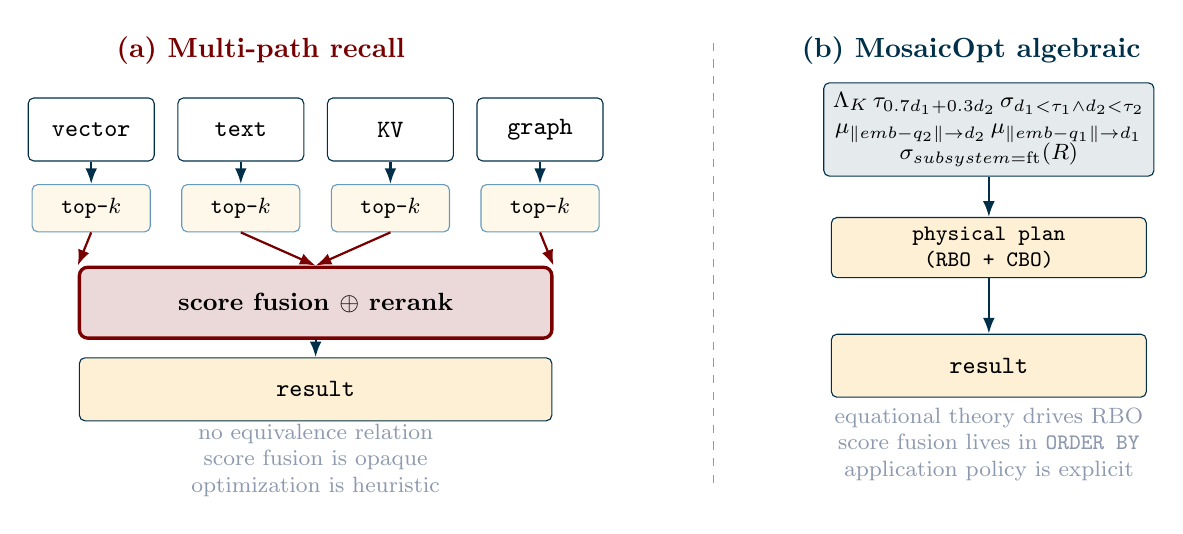
\begin{tikzpicture}[
    box/.style={rectangle, draw=mosaicBlue, fill=white, rounded corners=2pt, minimum height=0.8cm, font=\ttfamily\small, align=center},
    scorebox/.style={rectangle, draw=mosaicLightBlue, fill=mosaicCream!50, rounded corners=2pt, minimum height=0.6cm, font=\ttfamily\footnotesize, align=center},
    fusionbox/.style={rectangle, draw=mosaicCrimson, fill=mosaicCrimson!15, very thick, rounded corners=3pt, minimum height=0.9cm, font=\small\bfseries, align=center},
    planbox/.style={rectangle, draw=mosaicBlue, fill=white, rounded corners=2pt, minimum height=0.7cm, font=\ttfamily\footnotesize, align=center},
    arr/.style={-{Latex[length=2mm]}, thick, color=mosaicBlue},
    arr2/.style={-{Latex[length=2mm]}, thick, color=mosaicCrimson}
  ]
    % Left side: Multi-path recall
    \node[font=\bfseries, color=mosaicCrimson, anchor=west] at (-7.2,3.2) {(a) Multi-path recall};
    \node[box, minimum width=1.6cm] (v1) at (-7.4,2.2) {vector};
    \node[box, minimum width=1.6cm] (t1) at (-5.5,2.2) {text};
    \node[box, minimum width=1.6cm] (k1) at (-3.6,2.2) {KV};
    \node[box, minimum width=1.6cm] (g1) at (-1.7,2.2) {graph};
    \node[scorebox, minimum width=1.5cm] (vs1) at (-7.4,1.2) {top-$k$};
    \node[scorebox, minimum width=1.5cm] (ts1) at (-5.5,1.2) {top-$k$};
    \node[scorebox, minimum width=1.5cm] (ks1) at (-3.6,1.2) {top-$k$};
    \node[scorebox, minimum width=1.5cm] (gs1) at (-1.7,1.2) {top-$k$};
    \node[fusionbox, minimum width=6.0cm] (fu) at (-4.55,0.0) {score fusion $\oplus$ rerank};
    \node[box, fill=mosaicCream, minimum width=6.0cm] (res1) at (-4.55,-1.1) {result};
    \draw[arr] (v1) -- (vs1);
    \draw[arr] (t1) -- (ts1);
    \draw[arr] (k1) -- (ks1);
    \draw[arr] (g1) -- (gs1);
    \draw[arr2] (vs1.south) -- (fu.north west);
    \draw[arr2] (ts1.south) -- (fu.north);
    \draw[arr2] (ks1.south) -- (fu.north);
    \draw[arr2] (gs1.south) -- (fu.north east);
    \draw[arr] (fu) -- (res1);
    \node[font=\footnotesize, color=mosaicGray, align=center] at (-4.55,-2.0) {no equivalence relation \\ score fusion is opaque \\ optimization is heuristic};

    % Right side: MosaicOpt algebraic
    \node[font=\bfseries, color=mosaicBlue, anchor=west] at (1.5,3.2) {(b) MosaicOpt algebraic};
    \node[planbox, minimum width=4.0cm, fill=mosaicBlue!10] (log) at (4.0,2.2) {$\Lambda_K\,\tau_{0.7d_1+0.3d_2}\,\sigma_{d_1<\tau_1\wedge d_2<\tau_2}$ \\ $\mu_{\lVert emb-q_2\rVert\to d_2}\,\mu_{\lVert emb-q_1\rVert\to d_1}$ \\ $\sigma_{subsystem=\mathrm{ft}}(R)$};
    \node[planbox, minimum width=4.0cm, fill=mosaicCream] (cbo) at (4.0,0.7) {physical plan \\ \footnotesize (RBO + CBO)};
    \node[box, fill=mosaicCream, minimum width=4.0cm] (res2) at (4.0,-0.8) {result};
    \draw[arr] (log) -- (cbo);
    \draw[arr] (cbo) -- (res2);
    \node[font=\footnotesize, color=mosaicGray, align=center] at (4.0,-1.8) {equational theory drives RBO \\ score fusion lives in \texttt{ORDER BY} \\ application policy is explicit};

    % Vertical separator
    \draw[dashed, color=mosaicGray] (0.5,3.3) -- (0.5,-2.3);
  \end{tikzpicture}%
  }
  \Description{Side-by-side comparison: (a) Multi-path recall with four parallel boxes (vector, text, KV, graph) feeding into four top-k score lists, then a fusion box, then result; versus (b) MosaicOpt algebraic with one logical plan, one physical plan, then result.}
  \caption{Multi-path recall (a) versus the MosaicOpt algebraic approach (b).}
  \label{fig:multipath}
\end{figure}

Figure~\ref{fig:multipath} makes the contrast vivid. On the
left-hand side (a), four independent channels (vector, text,
key-value, graph) each produce a ranked candidate list, and
application-level score fusion decides the final ranking --- there
is no equivalence relation over plans, so all optimization is
heuristic. On the right-hand side (b), the user writes a single
logical plan over the extended algebra; the RBO enumerates
equivalent rewrites under the equational theory, and the CBO
picks a physical realization. The fusion policy is explicit in
the \texttt{ORDER BY} expression; the substrate has no opinion on
the weights.

% =====================================================================
% 3. The Extended Algebra
% =====================================================================
\section{The Extended Algebra: Syntax \& Semantics}\label{sec:algebra}

We extend the classical relational algebra with three new kinds of
construct: a \emph{materialization} operator that lifts computed
values to first-class attributes, first-class multi-modal predicates
(vector distance, BM25, graph reachability), and a \emph{graph
expansion} operator. Bag semantics are used throughout, matching SQL
and avoiding the row-collapse anomalies of set semantics in the
presence of duplicate memory units. The logical/physical separation
is enforced: physical operators are introduced in
Section~\ref{sec:cbo} and never appear in this section.

\subsection{Logical/physical separation}

Following System~R and Cascades, we treat the \emph{logical} algebra
as the substrate contract --- what the user asks for --- and the
\emph{physical} algebra as the engine contract --- how it is
evaluated. Equivalences hold in the logical algebra; physical
operators are \emph{implementations} of logical operators, and a
logical equivalence does not in general imply that two physical
realizations are interchangeable (Section~\ref{sec:equational:nonident},
N1--N3). This separation is what makes the system \emph{composable}:
HNSW can be added, swapped, or replaced without changing the language
the user sees.

\subsection{Operator inventory}

A \emph{logical plan} is a term over the following operators. $R$
denotes a stored base relation. $L$, $M$ denote logical plans.
$\varphi$ denotes a predicate, $e$ a materialization expression, $A$
a set of attribute names, $O$ an ordering expression, $K$ a
non-negative integer, $c$ a fresh attribute name, $g$ a graph rule
(a labelled-edge pattern), and $d$ a non-negative integer depth.

\begin{table}[t]
  \centering
  \scriptsize
  \begin{tabular}{@{}p{2.0cm}p{2.9cm}p{2.9cm}@{}}
    \toprule
    Operator & Syntax & Meaning \\
    \midrule
    Base relation & $R$ & The named stored relation. \\
    Selection & $\sigma_\varphi(L)$ & Keep rows satisfying $\varphi$. \\
    Projection & $\pi_A(L)$ & Keep only attributes in $A$. \\
    Materialization & $\mu_{e\to c}(L)$ & Per row, compute $e$; bind to $c$. \\
    Join & $L \bowtie_\psi M$ & Pair rows with $\psi$ true. \\
    Union / Inter / Diff & $L \cup M$, $L \cap M$, $L-M$ & Bag set ops on compat. schemas. \\
    Rename & $\rho_{a\to b}(L)$ & Rename attribute $a$ to $b$. \\
    Ordering & $\tau_O(L)$ & Order rows by expression $O$. \\
    Limit & $\Lambda_K(L)$ & First $K$ rows of an ordered input. \\
    Graph expansion & $\Gamma_{g,d}(L)$ & From node-id, traverse $g$ to depth $d$. \\
    \bottomrule
  \end{tabular}
  \caption{Logical operators of the extended algebra.}
  \label{tab:ops}
\end{table}

\begin{definition}[Bag semantics]\label{def:bag}
A relation is a multiset of tuples. All operators are
multiset-preserving: $\sigma$, $\mu$, $\Gamma$ preserve row
multiplicity; projection preserves multiplicity; set operations
combine multiplicities additively for $\cup$, by $\min$ for $\cap$,
and by subtraction (clamped at $0$) for $-$. $\tau_O$ produces a
totally ordered sequence; $\Lambda_K$ truncates it.
\end{definition}

Bag semantics was chosen because the substrate must be able to
express ``the same memory unit appears $N$ times'' (e.g. an episodic
trace where the same event is recorded with several slightly different
timestamps), and because it matches the SQL semantics that
application code already expects.

\subsection{Predicate forms}

A predicate $\varphi$ is a Boolean combination of atoms over the
attributes of the input plan. The atom forms are:

\begin{itemize}[leftmargin=*]
  \item \textbf{Classical.} $A = c$, $A < c$, $A > c$, $A \in S$ for
    constant or set $c$, $S$.
  \item \textbf{Vector.} $\lVert V_a - q \rVert < \tau$ where $V_a$ is
    a vector-valued attribute of the input, $q$ is a query-time bound
    parameter (a dense vector), and $\tau \geq 0$ is a distance
    threshold. Equality and other comparison operators are admissible;
    range ($< \tau$) is the most important form.
  \item \textbf{Text.} $\mathrm{BM25}(t, q) > \theta$ where $t$ is a
    text attribute, $q$ a query-time bound string, and $\theta$ a
    relevance threshold. We use the Okapi BM25 definition
    \cite{bm25} with parameters $(k_1, b)$ carried with the predicate.
  \item \textbf{Graph.} $\mathrm{reachable}(u, v)$ (boolean) and
    $\mathrm{edge}(u, v, \ell)$ (boolean; $\ell$ is a label or
    wildcard) for nodes $u, v$ in a graph attribute.
  \item \textbf{Boolean combinations.} $\varphi \wedge \psi$, $\varphi
    \vee \psi$, $\neg \varphi$, parentheses.
\end{itemize}

The \emph{query-time bound parameters} ($q$, $\tau$, $\theta$) are
first-class values supplied at execution time, distinct from
attributes of the input. They make predicates safely
\emph{late-binding}: the algebra expression is the same across query
instances, only the bound parameters change.

\subsection{Materialization expressions}

A materialization expression $e$ is computed per row and bound to a
fresh attribute name. Forms are:

\begin{itemize}[leftmargin=*]
  \item \textbf{Classical.} $A + B$, $f(A)$ for any scalar function $f$.
  \item \textbf{Vector.} $\lVert V_a - q \rVert$ --- the distance from
    a vector attribute to a query-time bound vector.
  \item \textbf{Text.} $\mathrm{BM25}(t, q)$ --- a BM25 score.
  \item \textbf{Boolean / arithmetic combinations} of the above.
\end{itemize}

The key property of $\mu$ is that the \emph{result} of the computation
becomes a first-class attribute of the output. Once materialized, the
value can be referenced by downstream $\sigma$, by $\pi$, by
\texttt{ORDER BY} expressions in $\tau$, and by other $\mu$
expressions. This is what makes the substrate able to expose
per-column distances to application-level \texttt{ORDER BY} without losing them.

\begin{definition}[Fresh-name condition]\label{def:fresh}
The new attribute name $c$ in $\mu_{e\to c}(L)$ must not already
appear in the schema of $L$. This is a hygiene condition, not a
semantic restriction; $\rho$ is provided to free names if needed.
\end{definition}

\subsection{Materialization: motivation and semantics}

A na\"ive way to expose per-column distances to the application is
to \emph{inline} them in \texttt{ORDER BY} expressions:
\texttt{ORDER BY} $\lVert V_a - q_a \rVert + \lVert V_b - q_b \rVert$.
This is syntactically permitted by SQL extensions, but it forces the
application to write the distance expression everywhere it is used,
and it leaves the optimizer no room to share computation between,
say, a \texttt{WHERE} filter and an \texttt{ORDER BY} rank.

$\mu$ resolves this. The pattern
\[
\mu_{\lVert V_a-q_a\rVert\to d_a}\;
\mu_{\lVert V_b-q_b\rVert\to d_b}\;
\sigma_{d_a < \tau_a \wedge d_b < \tau_b}\;
\tau_{d_a + d_b}\;
\Lambda_K
\]
says: ``compute the distance to query $a$ and to query $b$; keep
rows where both are below their respective thresholds; sort by sum
of distances; return the top $K$.'' The fusion policy $d_a + d_b$ is
expressed once, in the $\tau$ expression. The optimizer can rewrite
this plan --- for example, by using M1 to commute the selection
through the materializations, computing each distance only on
surviving rows (Section~\ref{sec:rbo}).

Formally, the semantics of $\mu_{e\to c}(L)$ is the multiset
$\{\, r \oplus \{c \mapsto e(r)\} : r \in L \,\}$, where $\oplus$
extends the tuple with the binding of the fresh attribute $c$ to
the value of $e$ on $r$. If $e(r)$ is undefined (e.g. distance to a
null vector), the row is dropped. This is a minor departure from
pure relational algebra, but it is consistent with SQL's
\texttt{NULL} handling and is essential for safety in the presence of
missing embeddings.

\subsection{Graph expansion}

$\Gamma_{g,d}(L)$ takes a plan whose rows contain a node-id attribute
($u$, say) and a graph attribute, applies graph rule $g$ up to depth
$d$, and returns the \emph{target} nodes of those traversals (joined
with the originating row). The depth is inclusive of intermediate
hops. $g$ is a labelled-edge pattern: a regular expression over edge
labels, evaluated against the graph. The graph itself is supplied as
a relation-valued attribute; the expansion is a join between $L$ and
the traversal result.

$\Gamma$ is intentionally narrow. We do not attempt to encode path
queries as selection predicates; this keeps the operator set small
and the rewrite theory tractable (Section~\ref{sec:equational}, G1).
Path information can be recovered by a $\mu$ that records the path
taken.

\subsection{Example queries}

We illustrate the algebra on a running example. Let $\Mem$ be a
relation of memory units with schema
\[
\begin{aligned}
\Mem(&\mathit{id}: \mathrm{int},\; \mathit{text}: \mathrm{string}, \\
     &\mathit{ts}: \mathrm{timestamp},\;
       \vect{emb}: \mathrm{vector},\;
       \vect{emb\_alt}: \mathrm{vector}, \\
     &\mathit{user}: \mathrm{string},\;
       \mathit{subsystem}: \mathrm{string}).
\end{aligned}
\]
Let $\KG$ be a graph relation
\[
\KG(\mathit{src}: \mathrm{int},\; \mathit{dst}: \mathrm{int},\;
    \mathit{label}: \mathrm{string})
\]
holding derivation links between memory units. The query ``find
semantically similar passages in the fault-tolerance subsystem from
the last 30 days, ranked by a weighted sum of two distance metrics,
top 10'' is
\begin{align*}
Q_1 &= \Mem, \\
Q_2 &= \sigma_{\mathit{subsystem} = \mathrm{`fault\text{-}tolerance'} \wedge \mathit{ts} > \mathrm{now}() - 30d}(Q_1), \\
Q_3 &= \mu_{\lVert\vect{emb} - \vect{q}_1\rVert \to d_1}\;
        \mu_{\lVert\vect{emb\_alt} - \vect{q}_2\rVert \to d_2}(Q_2), \\
Q_4 &= \sigma_{d_1 < \tau_1 \wedge d_2 < \tau_2}(Q_3), \\
Q_5 &= \tau_{0.7\cdot d_1 + 0.3\cdot d_2}(Q_4), \\
Q_6 &= \Lambda_{10}(Q_5).
\end{align*}

The fusion policy $0.7\cdot d_1 + 0.3\cdot d_2$ is application code;
the substrate has no opinion on the weights. The thresholds
$\tau_1, \tau_2$ are application choices too. The algebra's job is
to make this expression \emph{rewriteable} --- for example, to
compute $d_1$ and $d_2$ only on the post-selection rows, and to
enable \texttt{topK} early termination.

\begin{figure}[t]
  \centering
  \resizebox{\columnwidth}{!}{%
  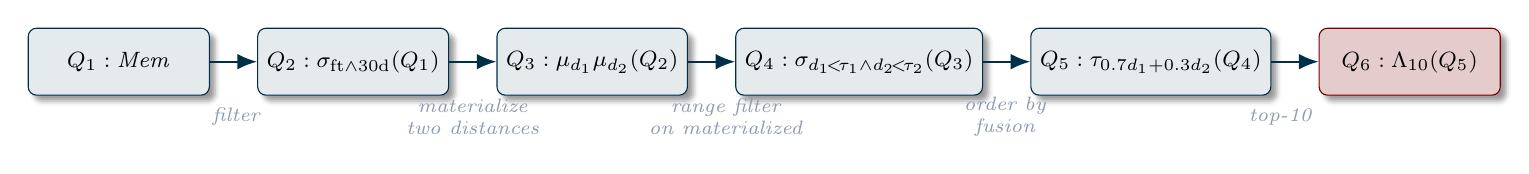
\begin{tikzpicture}[
    qbox/.style={rectangle, draw=mosaicBlue, fill=mosaicBlue!10, rounded corners=3pt, minimum width=2.3cm, minimum height=0.85cm, font=\ttfamily\footnotesize, align=center, blur shadow={shadow blur steps=3}},
    step/.style={rectangle, draw=mosaicCrimson, fill=mosaicCream!60, rounded corners=3pt, minimum width=1.6cm, minimum height=0.7cm, font=\scriptsize, align=center},
    ann/.style={font=\scriptsize\itshape, color=mosaicGray, align=center},
    arr/.style={-{Latex[length=2.5mm,width=2mm]}, thick, color=mosaicBlue}
  ]
    \node[qbox] (q1) at (0,0) {$Q_1: \Mem$};
    \node[qbox, right=0.6cm of q1] (q2) {$Q_2: \sigma_{\mathrm{ft}\wedge\mathrm{30d}}(Q_1)$};
    \node[qbox, right=0.6cm of q2] (q3) {$Q_3: \mu_{d_1}\mu_{d_2}(Q_2)$};
    \node[qbox, right=0.6cm of q3] (q4) {$Q_4: \sigma_{d_1\!<\!\tau_1\wedge d_2\!<\!\tau_2}(Q_3)$};
    \node[qbox, right=0.6cm of q4] (q5) {$Q_5: \tau_{0.7d_1+0.3d_2}(Q_4)$};
    \node[qbox, right=0.6cm of q5, fill=mosaicCrimson!20, draw=mosaicCrimson] (q6) {$Q_6: \Lambda_{10}(Q_5)$};
    \draw[arr] (q1) -- (q2);
    \draw[arr] (q2) -- (q3);
    \draw[arr] (q3) -- (q4);
    \draw[arr] (q4) -- (q5);
    \draw[arr] (q5) -- (q6);

    % Annotations under the arrows
    \node[ann] at ($(q1)!0.5!(q2) + (0,-0.7)$) {filter};
    \node[ann] at ($(q2)!0.5!(q3) + (0,-0.7)$) {materialize\\two distances};
    \node[ann] at ($(q3)!0.5!(q4) + (0,-0.7)$) {range filter\\on materialized};
    \node[ann] at ($(q4)!0.5!(q5) + (0,-0.7)$) {order by\\fusion};
    \node[ann] at ($(q5)!0.5!(q6) + (0,-0.7)$) {top-10};
  \end{tikzpicture}%
  }
  \Description{Horizontal pipeline with six boxes: Q1 (base relation Mem), Q2 (filter on subsystem and timestamp), Q3 (materialize two distances), Q4 (range filter), Q5 (order by fusion), Q6 (top-10). Arrows between boxes show data flow.}
  \caption{The running example $Q_1 \to Q_6$ as a horizontal pipeline.}
  \label{fig:pipeline}
\end{figure}

Figure~\ref{fig:pipeline} renders the same example as a horizontal
pipeline. Each box is a logical plan; the arrows denote data flow.
The visual emphasises the compositionality of the algebra: each
$Q_i$ is itself a logical plan and can be referenced as input to
the next. The fusion policy $0.7\cdot d_1 + 0.3\cdot d_2$ lives in
the $\tau$ operator of $Q_5$; the substrate has no opinion on the
weights. The optimizer uses M1 to push $Q_4$'s selection below
$Q_3$'s materializations, computing $d_1$ and $d_2$ only on rows
that survive the filter.

A graph-aware variant --- ``the same, but only memories linked by a
\texttt{derived\_from} chain to a known incident memory'' --- is
\begin{align*}
R_1 &= \sigma_{\mathit{id} = 42}(\Mem) &&\text{--- the seed incident} \\
R_2 &= \Gamma_{\mathit{label}=\mathrm{`derived\_from'},\, d=2}(R_1) &&\text{--- two hops downstream} \\
R_3 &= \sigma_{\mathit{id} \in \pi_{\mathit{dst}}(R_2)}(Q_2) &&\text{--- intersect with subsystem filter}
\end{align*}
followed by the same materialization / selection / ordering / limit
chain as before. The graph expansion is composable: $\Gamma$ produces
a relation that can be $\sigma$-, $\pi$-, and $\mu$-ed like any
other.

% =====================================================================
% 4. Equational Theory: Identities and Non-Identities
% =====================================================================
\section{Equational Theory: Identities and Non-Identities}\label{sec:equational}

The optimizer (Section~\ref{sec:rbo}) is driven by an
\emph{equational theory}: a set of identities over logical plans.
The same theory also records, explicitly, the identities that
classical intuition suggests but approximation breaks --- the
\emph{non-identities} --- so the optimizer knows not to apply them.
This section unifies both sides. We first give an overview
(4.1), then the inherited classical axioms (4.2), then the new
identities that the extended operators license (4.3), then the
derived rewrites the optimizer uses (4.4), and finally the
non-identities with counterexamples (4.5).

\subsection{Overview}\label{sec:equational:overview}

The equational theory of the extended algebra plays two
complementary roles. \emph{First}, it is the foundation for the
rule-based optimizer (Section~\ref{sec:rbo}): every rewrite the
RBO performs is justified by a foundational identity (M1--M5, G1,
G2) or by a derived corollary / definitional / implied rule (A4-vector,
A4-vector+M1, M4+M1, M5+G1, A7-symmetry, A8-regroup, $\topK$
recognition, $\sigma$-$\tau$ commutation) --- so the optimizer's
behaviour is auditable, not opaque. \emph{Second}, the
\emph{non}-identities (N1--N5) are the discipline that prevents
the optimizer from applying rewrites that hold in classical
relational algebra but break under approximation, graph-traversal
asymmetry, or the traversal-vs-origin column split. The cost model
(Section~\ref{sec:cbo}) is responsible for the physical cost of
every rewrite; the equational theory is responsible for its
\emph{correctness}.

Concretely, an identity is an equation of the form
\texttt{LHS = RHS} between two logical plans that hold for all
instances of the free variables (relation names, attribute names,
query-time bound parameters). A non-identity is a pair of plans
that classical intuition might equate but the extended setting
does not, with an explicit counterexample. Both are first-class
objects: the RBO loads them as data, the cost model consults them
when computing the ``cost of identity application'' term, and the
executor relies on them for safety of adaptive re-planning
(Section~\ref{sec:cbo}).

The structure of this section follows the algebra's structure:
inherited axioms (the ones we use but do not re-prove) in
Section~\ref{sec:equational:inherited}; new identities (the ones
the extended operators license) in
Section~\ref{sec:equational:new}; derived rules (combinations used
directly by the optimizer) in
Section~\ref{sec:equational:derived}; and non-identities
(counterexamples that bound the optimization horizon) in
Section~\ref{sec:equational:nonident}.

\subsection{Inherited foundational axioms}\label{sec:equational:inherited}

The following identities are standard and are assumed without
re-proof. We list them because they interact with the new identities
in Section~\ref{sec:rbo}. The list includes the two classical
join-reordering identities (A7, A8) because the RBO uses them to
enumerate the $O(n!)$ join orderings of
Section~\ref{sec:rbo:complexity}.

\begin{itemize}[leftmargin=*]
  \item \textbf{(A1) Selection composition.}
    $\sigma_\varphi \sigma_\psi(L) = \sigma_{\varphi \wedge \psi}(L)$.
  \item \textbf{(A2) Selection distributes over union.}
    $\sigma_\varphi(L \cup M) = \sigma_\varphi(L) \cup \sigma_\varphi(M)$.
  \item \textbf{(A3) Projection idempotence.}
    $\pi_A \pi_B(L) = \pi_A(L)$ if $A \supseteq B$.
  \item \textbf{(A4) Selection--join pushdown.} If every attribute
    mentioned in $\varphi$ is in the schema of $L$, then
    $\sigma_\varphi(L \bowtie_\psi M) = \sigma_\varphi(L) \bowtie_\psi M$.
  \item \textbf{(A5) Projection--join pushdown.} If $A$ contains all
    attributes of $L$ and all attributes referenced by $\psi$ in $M$,
    then $\pi_A(L \bowtie_\psi M) = \pi_A(L) \bowtie_\psi
    \pi_{A \,\cap\, \attr{M}}(M)$.
  \item \textbf{(A6) Rename is involutive on attribute names.}
    $\rho_{b\to a}(\rho_{a\to b}(L)) = L$.
  \item \textbf{(A7) Join commutativity.} For any join predicate
    $\psi$ that depends only on attributes of $L$ and $M$
    symmetrically (the case for every equality, range, similarity,
    and Boolean-combination predicate in the inventory):
    $L \bowtie_\psi M = M \bowtie_{\psi^{\mathrm{sym}}} L$ where
    $\psi^{\mathrm{sym}}$ swaps the $L$- and $M$-side attribute
    references in $\psi$. Logically the two sides are identical as
    multisets; the cost of evaluating them is not
    (Theorem~\ref{thm:n2}).
  \item \textbf{(A8) Join associativity.} For independent join
    predicates $\psi$ (between $L$ and $M$) and $\chi$ (between
    $L \cup M$ and $N$), where $\chi$ does not reference any
    attribute introduced by $L$ or $M$ (no ambiguity):
    $L \bowtie_\psi (M \bowtie_\chi N) = (L \bowtie_\psi M) \bowtie_\chi N$.
    This is the identity the RBO uses to enumerate the $O(n!)$ join
    orderings; without it, commutativity alone yields only $O(n)$
    swaps on a fixed parenthesization.
\end{itemize}

These hold for any predicate $\varphi$ in our extended form
(classical, vector, text, graph), provided the attribute references
are respected. We do not claim any \emph{new} identities here; we
merely note that the extended predicates do not violate them.

\subsection{New foundational axioms}\label{sec:equational:new}

We introduce the \emph{seven} identities that the extended algebra
makes possible. Each is stated in a form that names the conditions
for its applicability. (Two further rules --- \textbf{V1} and
\textbf{J1} --- are corollaries of the assumed classical axioms
A1 and A4 with vector-predicate specialization; they are kept as
named redex patterns in the RBO code but have no separate theorem
block. The $\tau$-$\Lambda$-$\topK$ family and the
$\sigma$-$\tau$ commutation are \emph{implied} by the operator
definitions: $\topK_O(L, K) := \tau_O(\Lambda_K(L))$ from
Section~\ref{sec:algebra} and the row-preserving semantics of
$\sigma$ and $\tau$. The RBO uses them as zero-weight rewrites in
the ARS, but they have no separate theorem block.)

Each identity below is followed by a brief \emph{cost-effect
annotation} that names the optimization the rewrite enables; the
RBO fires the rewrite as part of its greedy loop
(Section~\ref{sec:rbo:role}).

\begin{theorem}[M1 --- Selection commutes with materialization on the materialized column]\label{thm:m1}
Where $c$ is a fresh attribute name and $e$ is an expression
depending only on attributes of $L$:
\[
\sigma_{c < \tau}\, \mu_{e \to c}(L) \;=\; \mu_{e \to c}\, \sigma_{e < \tau}(L).
\]
\end{theorem}

\begin{proof}
Fix $r \in L$. The LHS computes $e(r)$, attaches it as $c$, and
retains $r \oplus \{c \mapsto e(r)\}$ iff $e(r) < \tau$. The RHS
evaluates $e(r) < \tau$ directly: if false, $r$ is dropped; if true,
the row is extended to $r \oplus \{c \mapsto e(r)\}$ by the $\mu$.
The two multisets are equal row-by-row. The freshness of $c$ ensures
that the predicate $c < \tau$ in LHS is unambiguous --- $c$ is defined
by the $\mu$ and is not shadowed by any pre-existing attribute.
\qed
\end{proof}

\begin{figure}[t]
  \centering
  \resizebox{\columnwidth}{!}{%
  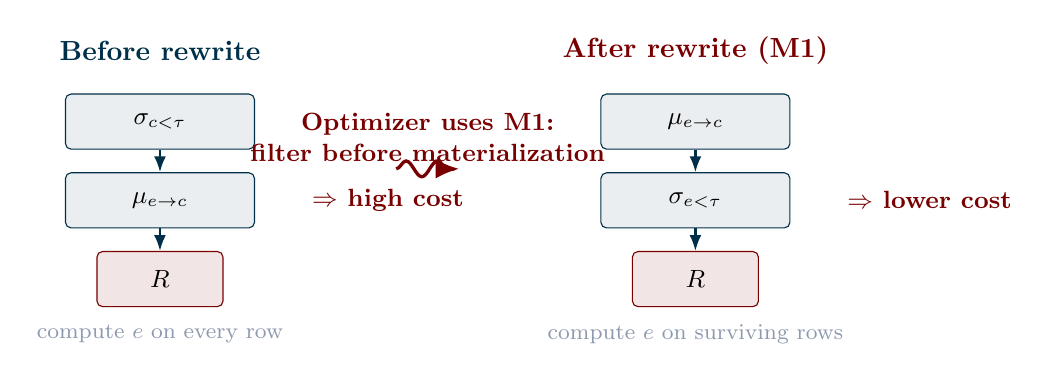
\begin{tikzpicture}[
    node distance=0.4cm and 0.6cm,
    op/.style={rectangle, draw=mosaicBlue, fill=mosaicBlue!8, rounded corners=2pt, minimum width=2.4cm, minimum height=0.7cm, font=\ttfamily\small, align=center},
    rnode/.style={rectangle, draw=mosaicCrimson, fill=mosaicCrimson!10, rounded corners=2pt, minimum width=1.6cm, minimum height=0.7cm, font=\ttfamily\small, align=center},
    arr/.style={-{Latex[length=2mm]}, thick, color=mosaicBlue},
    ann/.style={font=\footnotesize, color=mosaicGray, align=center},
    cost/.style={font=\small\bfseries, color=mosaicCrimson}
  ]
    % Left tree (before rewrite)
    \node[font=\bfseries, color=mosaicBlue] at (-3.4, 2.4) {Before rewrite};
    \node[op] (leftsigma) at (-3.4, 1.5) {$\sigma_{c<\tau}$};
    \node[op] (leftmu) at (-3.4, 0.5) {$\mu_{e\to c}$};
    \node[rnode] (leftR) at (-3.4, -0.5) {$R$};
    \draw[arr] (leftsigma) -- (leftmu);
    \draw[arr] (leftmu) -- (leftR);
    \node[ann, below=0.1cm of leftR] {compute $e$ on every row};
    \node[cost, right=0.0cm of leftmu, xshift=0.6cm] {$\Rightarrow$ high cost};

    % Right tree (after rewrite)
    \node[font=\bfseries, color=mosaicCrimson] at (3.4, 2.4) {After rewrite (M1)};
    \node[op] (rightmu) at (3.4, 1.5) {$\mu_{e\to c}$};
    \node[op] (rightsigma) at (3.4, 0.5) {$\sigma_{e<\tau}$};
    \node[rnode] (rightR) at (3.4, -0.5) {$R$};
    \draw[arr] (rightmu) -- (rightsigma);
    \draw[arr] (rightsigma) -- (rightR);
    \node[ann, below=0.1cm of rightR] {compute $e$ on surviving rows};
    \node[cost, right=0.0cm of rightsigma, xshift=0.6cm] {$\Rightarrow$ lower cost};

    % Optimization arrow
    \draw[-{Latex[length=3mm,width=2.5mm]}, very thick, color=mosaicCrimson, decorate, decoration={snake, amplitude=1mm, segment length=4mm}] (-0.4,0.9) -- (0.4,0.9);
    \node[ann, color=mosaicCrimson, font=\small\bfseries] at (0,1.3) {Optimizer uses M1:\\filter before materialization};
  \end{tikzpicture}%
  }
  \Description{Two tree diagrams side by side. Left (before rewrite): $\sigma_{c<\tau}$ on top of $\mu_{e\to c}(R)$ — both $e$ computation and filtering happen. Right (after rewrite): $\mu_{e\to c}$ on top of $\sigma_{e<\tau}(R)$ — filter first, then compute. Annotation: cost saving is that $e$ is computed only on rows that survive the filter.}
  \caption{Visualization of the M1 rewrite.}
  \label{fig:m1}
\end{figure}

Figure~\ref{fig:m1} visualizes the M1 rewrite. The \emph{left} tree
shows the input plan: $\sigma_{c<\tau}$ on top of $\mu_{e\to c}(R)$,
which materializes $e$ on every row and then filters on $c < \tau$.
The \emph{right} tree shows the rewritten plan: $\mu_{e\to c}$ on
top of $\sigma_{e<\tau}(R)$, which applies the filter
\emph{before} materialization; $e$ is computed only on rows that
survive the filter. The cost saving scales with the selectivity
of $e < \tau$ --- for a tight vector range the selectivity can be
one part in $10^3$ or smaller, and the saving is correspondingly
dramatic.

\begin{theorem}[M2 --- Materialization is commutative]\label{thm:m2}
For fresh names $c_1, c_2$ and expressions $e_1, e_2$ depending
only on $L$'s attributes (and not on each other's outputs):
\[
\mu_{e_1 \to c_1}\, \mu_{e_2 \to c_2}(L)
\;=\;
\mu_{e_2 \to c_2}\, \mu_{e_1 \to c_1}(L).
\]
\end{theorem}

\begin{proof}
For each $r \in L$, LHS computes $e_1(r)$ and then $e_2(r)$, attaching
both; RHS computes $e_2(r)$ and then $e_1(r)$. Because $e_1$ and
$e_2$ depend only on $r$ and not on each other's intermediate
result, the two sequences yield the same extension $r \oplus \{c_1
\mapsto e_1(r), c_2 \mapsto e_2(r)\}$. The multisets are equal. \qed
\end{proof}

\begin{theorem}[M3 --- Materialization through projection]\label{thm:m3}
For fresh $c$ and expression $e$ depending only on attributes in $A$:
\[
\mu_{e \to c}\, \pi_A(L) \;=\; \pi_{A \cup \{c\}}\, \mu_{e \to c}(L).
\]
\end{theorem}

\begin{proof}
For $r \in L$, the LHS produces $\pi_A(r) \oplus \{c \mapsto
e(\pi_A(r))\}$. The RHS produces $r \oplus \{c \mapsto e(r)\}$ (using
the same $e$ since $e$ depends only on $A$), then projects to
$(A \cup \{c\})$. By the support of $e$, $e(r) = e(\pi_A(r))$, and
the resulting tuples agree. The freshness of $c$ ensures the
projection is well-formed. \qed
\end{proof}

\begin{theorem}[M4 --- Materialization pushdown through join]\label{thm:m4}
Where $e$ depends only on attributes of $L$ and $c$ is a fresh
attribute name:
\[
\mu_{e \to c}\, (L \bowtie_\psi M)
\;=\;
(\mu_{e \to c}(L)) \bowtie_\psi M.
\]
\end{theorem}

\begin{proof}
Fix a row $(r_L, r_M) \in L \bowtie_\psi M$ such that
$\psi(r_L, r_M)$ holds. The LHS produces
$(r_L, r_M) \oplus \{c \mapsto e(r_L)\}$. The RHS first
materializes $L$ to obtain
$\mu_{e \to c}(L) = \{r_L' \oplus \{c \mapsto e(r_L')\} : r_L' \in L\}$,
then joins with $M$ on $\psi$; since $c$ is fresh and not referenced
by $\psi$ (Def.~fresh), the result is
$\{ (r_L', r_M) \oplus \{c \mapsto e(r_L')\} : r_L' \in L, r_M \in M,
\psi(r_L', r_M) \}$. Because $e$ depends only on $L$'s attributes,
the materialized value $e(r_L)$ is computed in both cases from
the same $r_L$, and $\psi$ is unaffected by the addition of $c$ to
$L$'s schema. The two multisets agree row-by-row. \qed
\end{proof}

\begin{theorem}[M5 --- Materialization pushdown through graph expansion]\label{thm:m5}
Where $e$ depends only on attributes of $L$, $c$ is fresh, and $c$
is not the graph rule's node-id attribute:
\[
\mu_{e \to c}\, \Gamma_{g, d}(L)
\;=\;
\Gamma_{g, d}\, \mu_{e \to c}(L).
\]
This is the $\mu$-counterpart of G1 and the rewrite the RBO
generates for graph queries that materialize a per-origin attribute
(e.g.\ a distance to a fixed query point) and then expand. The
two sides produce the same multiset of $(r, v, c)$ tuples; the
cost differs because the LHS computes $e$ on every traversal row
while the RHS computes $e$ on every origin row. When
$|\Gamma_{g,d}(L)| > |L|$ (the typical case for $d \geq 1$ and a
non-trivial graph), the RHS is cheaper, and the CBO picks it.
\end{theorem}

\begin{proof}
For each row $r \in L$, the LHS first expands $r$ via $\Gamma_{g,d}$
to obtain a multiset $\{(r, v_i) : v_i \text{ reachable from } r
\text{.id by } g \text{ within } d\}$ (multiplicity = number of
paths), then materializes $e$ on each traversal row. The result is
the multiset $\{(r, v_i, c) : r \in L, v_i \text{ reachable from } r,
c = e(r)\}$, where $e$ depends only on $r$'s attributes by the
support condition. The RHS first materializes $e$ on $L$ to obtain
$\mu_{e \to c}(L) = \{r \oplus \{c \mapsto e(r)\} : r \in L\}$, then
expands via $\Gamma_{g,d}$. Because $c$ is fresh and is not the
graph rule's node-id attribute, the expansion proceeds from the
original node-id (unchanged by the $\mu$); the result is
$\{((r, c), v_i) : r \in L, v_i \text{ reachable from } r\text{.id}\}$.
Reordering attributes, this is
$\{(r, v_i, c) : r \in L, v_i \text{ reachable from } r, c = e(r)\}$,
the same multiset as the LHS. The two multisets agree row-by-row.
\qed
\end{proof}

\begin{theorem}[G1 --- Selection pushdown through graph expansion]\label{thm:g1}
Where $\varphi$ references only attributes of $L$ (and not
attributes of the graph rule's traversal result):
\[
\sigma_\varphi\, \Gamma_{g, d}(L) \;=\; \Gamma_{g, d}\, \sigma_\varphi(L).
\]
\end{theorem}

\begin{proof}
The graph expansion $\Gamma_{g,d}$ is \emph{row-multiplicating}: each
origin row $r \in L$ produces one or more traversal rows in the
result, and the multiplicity of $r$'s descendants is preserved
(i.e.\ $\Gamma_{g,d}$ does not collapse duplicates introduced by
$L$). Let $R \subseteq L$ be the multiset of rows satisfying
$\varphi$. The LHS starts from $L$ and applies $\sigma_\varphi$
\emph{after} expansion, so any traversal row whose origin row lies
outside $R$ is removed; the RHS starts from $R$ and only
generates traversal rows whose origin satisfies $\varphi$, so
none are removed. The multisets agree row-by-row, because
$\varphi$ references only origin attributes --- if $\varphi$
referenced traversal attributes, the two sides would diverge and
the identity would fail. \qed
\end{proof}

\begin{theorem}[G2 --- Graph expansion is transitive]\label{thm:g2}
Let $g_1, g_2$ be graph rules over the same graph attribute
with disjoint label sets. If $g_1$'s traversal-result
attribute and $g_2$'s source attribute are disjoint (no
intermediate node of $g_2$ is a valid origin of $g_1$),
then the composition $g_1 ; g_2$ satisfies:
\[
\Gamma_{g_1, d_1}\, \Gamma_{g_2, d_2}(L) \;=\;
\Gamma_{g_1;g_2,\, d_1+d_2}(L).
\]
\emph{Cost effect:} the LHS performs two graph walks (one of
depth $d_1$, one of depth $d_2$, each visiting a separate
frontier set of nodes) and materializes their intermediate
result; the RHS performs a single walk of depth $d_1 + d_2$
through the composite rule. For a graph with branching factor
$b$, the LHS visits $\sum_{i=0}^{d_1} b^i \cdot b^{d_2}$ nodes
across both walks (with intermediate expansion materialization
in between), while the RHS visits $\sum_{i=0}^{d_1+d_2} b^i$ nodes
in a single walk. G2 lets the RBO collapse nested
$\Gamma$s into a single expansion at depth $d_1 + d_2$
--- ``two \texttt{derived\_from} hops'' becomes ``one
\texttt{derived\_from} ; \texttt{derived\_from} hop''.
\end{theorem}

\begin{proof}
For each $r \in L$, the LHS expands $r$ by $g_2$ to depth $d_2$
yielding rows $(r, v_2)$, then expands each $(r, v_2)$ by
$g_1$ to depth $d_1$ yielding $(r, v_2, v_1)$ for each $v_1$
reachable from $v_2$. The RHS expands $r$ by $g_1;g_2$ to
depth $d_1 + d_2$, yielding $(r, v_1)$ for each $v_1$
reachable from $r$ by the composite. By the disjoint-label
condition, $g_1$'s traversal starts at $v_2$ and ends at
$v_1$, independent of $r$'s attributes; collapsing
intermediate $v_2$ in the LHS gives the same $(r, v_1)$
multiset as the RHS. The non-overlap condition
($g_1$'s traversal result disjoint from $g_2$'s source)
ensures no join is needed; without it, the LHS would
require a join between $g_2$'s targets and $g_1$'s origins.
\qed
\end{proof}

The G2 collapse is bounded by the number of nested-$\Gamma$
inversions in $P$ (one collapse per nesting, hence the depth $d$
of the result). G2 is a zero-weight rewrite: it does not change
the logical multiset, only the structure of the graph walk.

\subsection{Derived identities}\label{sec:equational:derived}

By composing the foundational axioms and the assumed classical
identities, additional rewrites become available. The optimizer
uses these directly; we list them as corollaries rather than as
standalone foundational theorems to keep
Section~\ref{sec:equational:new} focused on the genuinely new
content.

\begin{itemize}[leftmargin=*]
  \item \textbf{A4-vector (in code: \texttt{J1}).} A4 specialized
    to a vector predicate ---
    $\sigma_{\lVert V_a - q \rVert < \tau}\,(L \bowtie_\psi M) =
    (\sigma_{\lVert V_a - q \rVert < \tau}(L)) \bowtie_\psi M$
    when $V_a \in \attr{L}$ --- is what the CBO applies on the
    conjunctive multi-vector case. A1 likewise specializes to
    two vector predicates on distinct columns; the codebase
    calls this \texttt{V1}. Neither is a new algebraic identity
    --- both follow from A1/A4 by predicate substitution ---
    but the codebase keeps them as named redex patterns
    (\texttt{V1}, \texttt{J1}) so the RBO can match them
    explicitly without re-implementing A1/A4.
  \item \textbf{M4+M1 (materialization pushdown, then
    selection-on-materialized).} A join-side materialization
    can be reordered so the expensive per-row computation runs
    only on rows that survive the join's downstream filter:
    $\sigma_{c<\tau}\,\mu_{e\to c}\,(L\bowtie M) \;\equiv\;
    \mu_{e\to c}\,(\sigma_{e<\tau}(L)\bowtie M)$ (apply M4 then
    M1). \emph{Cost effect:} if the join has selectivity $s$
    and the materialization runs in $T_\mu$ per row, the rewrite
    saves $(1 - s) \cdot |L| \cdot T_\mu$ work. This is the
    rewrite that powers the $Q_1 \to Q_6$ running example:
    the distance is computed only on the surviving $L$ rows,
    not on every row of the join.
  \item \textbf{M5+G1 (materialization and selection through graph
    expansion).} A graph query with both a row-level filter and a
    row-level materialization can be reordered:
    $\sigma_\varphi\, \mu_{e\to c}\, \Gamma_{g,d}(L) \;\equiv\;
    \mu_{e\to c}\, \Gamma_{g,d}\, \sigma_\varphi(L)$ (apply G1
    then M5). \emph{Cost effect:} if the filter has selectivity
    $s$ against the post-expansion row count, the rewrite saves
    a factor of $1 - s$ in materialization work. The G2 collapse
    applied on top can then fold any resulting nested $\Gamma$s
    into a single graph walk of combined depth.
  \item \textbf{A4-vector+M1 (vector selection before materialization).}
    Combining A4-vector (J1) and M1 allows a join-side vector
    selection to be pushed below a materialization that binds a
    distance for sorting:
    \begin{align*}
      \sigma_{\lVert V-q\rVert<\tau}\; \mu_{\lVert V-q\rVert\to d}\; (L \bowtie M)
      &= \mu_{\lVert V-q\rVert\to d}\;
         \sigma_{\lVert V-q\rVert<\tau}\;(L \bowtie M)
         \quad\text{(M1)} \\
      &= \mu_{\lVert V-q\rVert\to d}\;
         \bigl(\sigma_{\lVert V-q\rVert<\tau}(L) \bowtie M\bigr)
         \quad\text{(A4-vector)}
    \end{align*}
    The plan now computes the distance only on the surviving
    $L$ rows. Same cost effect as M4+M1, but with the vector
    selection specifically.
  \item \textbf{A7-symmetry (reverse join).} Applying the assumed
    classical A7 in the reverse direction is a derived rewrite the
    RBO generates; the CBO then chooses the cheaper side per
    Theorem~\ref{thm:n2}.
  \item \textbf{A8-regrouping (different join parenthesization).}
    Applying the assumed classical A8 is the rewrite that exposes
    a different join parenthesization; the RBO uses it to
    enumerate the $O(n!)$ join orderings the CBO picks from.
  \item \textbf{$\topK$ recognition (definitional).} The
    abbreviation $\topK_O(L, K) := \tau_O(\Lambda_K(L))$ from
    Section~\ref{sec:algebra} makes
    $\tau_O\,\Lambda_K \leftrightarrow \topK_O$ a definitional
    rewrite; the CBO applies it as a physical-realization choice
    rather than as a logical RBO rewrite.
  \item \textbf{$\sigma$-$\tau$ commutation (implied by
    row-preserving semantics).} The identity
    $\sigma_\varphi\, \tau_O(L) = \tau_O\, \sigma_\varphi(L)$ holds
    trivially: $\sigma$ removes rows and $\tau$ rearranges them,
    neither changes the multiset of selected rows. The RBO applies
    it as a zero-weight $\sigma$-$\tau$ reordering bounded by the
    number of $\sigma$-$\tau$ inversions in $P$, letting the CBO
    pick filter-first or sort-first by selectivity.
    \emph{Cost effect:} filter-first avoids a full sort over
    rows that will be discarded; sort-first enables top-$K$
    early termination when paired with a downstream $\Lambda$.
\end{itemize}

The algebra is closed under composition: the output of any operator
is a logical plan usable as input to any other. The schema rules
ensure that the attributes a downstream operator references are
either attributes of the input or have been introduced by a $\mu$ in
the pipeline. The seven foundational axioms, the assumed classical
identities A1--A8, the derived rewrites above, and the two
implied-by-operator-definition rules ($\topK$ and $\sigma$-$\tau$)
together suffice to cover the optimization of all plans whose
operators draw from the inventory of
Section~\ref{sec:algebra}.

\begin{theorem}[RBO Confluence]\label{thm:rbo-confluence}
For any starting logical plan $P$ and any two RBO rewrite
sequences $P \to^*_{\mathrm{RBO}} P^*$ and
$P \to^*_{\mathrm{RBO}} P^{**}$, there exists a plan $P^\infty$
with $P^* \to^*_{\mathrm{RBO}} P^\infty$ and $P^{**}
\to^*_{\mathrm{RBO}} P^\infty$. The normal form is unique: it
depends only on $P$, not on rewrite order.
\end{theorem}

\begin{proof}
The ARS $\to_{\mathrm{RBO}}$ is the union of the seven
foundational rewrites (M1--M5, G1, G2) with the classical A1--A8
and the derived / implied rules above, oriented toward the
optimized form. \textbf{Termination}: M1, M3, M4, G1 strictly
decrease a weight function $w$ that counts, for a plan $P$,
the number of $\sigma$s on $\mu$-bound attributes, the number
of redundant $\mu$s, and the number of $\pi$s that drop needed
attributes. M2, M5, \textbf{G2}, and the implied $\sigma$-$\tau$
rewrite are zero-weight: M2 is a $\mu$-reorder bounded by the
$k!$ orderings of $k$ materializations; M5 is a
$\mu$-$\Gamma$ reorder bounded by the number of
$\mu$-$\Gamma$ inversions; \textbf{G2 is a $\Gamma$-$\Gamma$
collapse} bounded by the number of nested-$\Gamma$ inversions
(one collapse per nesting); the $\sigma$-$\tau$ rewrite is
bounded by the number of $\sigma$-$\tau$ inversions. The
$\topK$ recognition ($\tau_O\,\Lambda_K \leftrightarrow
\topK_O$ per the definition
$\topK_O(L, K) := \tau_O(\Lambda_K(L))$) is a definitional
rewrite applied by the CBO as a physical-realization choice
(in one-to-one correspondence with its inverse, so it
trivially terminates). Once $w$ reaches a local minimum,
only the zero-weight rewrites remain, and each terminates
by its bounded inversion count. \textbf{Local confluence}: the
critical pairs from overlapping redexes
(M1$\cap$M1, M1$\cap$M4, M1$\cap$G1, M1$\cap$M5,
M4$\cap$G1, M4$\cap$M5, M5$\cap$G1, G1$\cap$A4,
\textbf{G2$\cap$G2, G2$\cap$G1, G2$\cap$M5},
M2$\cap$M1, M2$\cap$M5, $\sigma$-$\tau$ $\cap$ M1,
$\sigma$-$\tau$ $\cap$ M3) all join by further rewrites,
giving local confluence. The G2$\cap$G2 pair joins by a
single G2 collapse (the outermost redex fires first; the
resulting $\Gamma_{g_1;g_2,d_1+d_2}$ has no remaining
$\Gamma$-$\Gamma$ redex). G2$\cap$G1 joins by G1 then G2
($\sigma$ pushes through the inner $\Gamma$, then the outer
collapse). G2$\cap$M5 joins by M5 then G2 ($\mu$ moves past
the inner $\Gamma$ first, then collapse). (A1-vector and
A4-vector --- V1, J1 in the codebase --- are A1/A4 applied to
vector predicates and do not produce new critical pairs beyond
those of A1, A4.) By Newman's lemma, termination plus
local confluence implies confluence, and the normal form is
unique. \qed
\end{proof}

Theorem~\ref{thm:rbo-confluence} is the formal correctness
guarantee of the RBO --- the optimizer can be implemented as
a simple greedy loop (apply any rule that decreases $w$)
without losing correctness. The CBO inherits confluence
``for free'': its search is over the unique canonical form,
so its choice of physical realization is well-defined and
reproducible.

\paragraph{Algorithm-level view of $\to_{\mathrm{RBO}}$.}
Concretely, the RBO is implemented as a Cascades-style
exploration engine
(Section~\ref{sec:rbo}). Algorithm~\ref{alg:rbo} gives the
top-level loop.

\begin{algorithm}[t]
\caption{RBO fixed-point loop with priority-ordered matchers.}\label{alg:rbo}
\textbf{Input:} a logical plan $P$; the matcher list
$\mathcal{M} = (\mathrm{M1}, \mathrm{M3}, \mathrm{M4},
\mathrm{G1}, \mathrm{G2}, \mathrm{M5}, \mathrm{M2},
\mathrm{V1}, \mathrm{J1}, \mathrm{T1})$; a
\texttt{max\_iters} safety bound (default 64).
\textbf{Output:} the rewritten plan $P'$ (the
canonical-form representative of $[P]_{\to_{\mathrm{RBO}}}$);
the trace $\tau$ of applied rule names.
\begin{algorithmic}[1]
  \State $\tau \gets []$
  \Repeat
    \State $\mathit{changed} \gets \textsc{false}$
    \For{each node $n$ in $P$ in \emph{preorder}}
      \For{each matcher $m_i \in \mathcal{M}$ in priority order}
        \If{$m_i.\Call{Match}{n}$ returns a rewrite $n'$}
          \State $n \gets n'$
          \State $\tau.\Call{Append}{m_i.\textsc{Name}}$
          \State $\mathit{changed} \gets \textsc{true}$
          \State \textbf{break} \Comment{re-traverse from this node}
        \EndIf
      \EndFor
    \EndFor
  \Until{$\mathit{changed} = \textsc{false}$ \textbf{or} $|\tau| = \texttt{max\_iters}$}
  \State \Return $P, \tau$
\end{algorithmic}
\end{algorithm}

\noindent\textbf{Three properties the loop relies on.}

\begin{enumerate}[leftmargin=*, itemsep=0pt]
  \item \textbf{Matcher priority order is a heuristic
  short-circuit, not a semantic guarantee.} The matchers
  are tried in the order
  $(\mathrm{M1}, \mathrm{M3}, \mathrm{M4}, \mathrm{G1},
  \mathrm{G2}, \mathrm{M5}, \mathrm{M2}, \mathrm{V1},
  \mathrm{J1}, \mathrm{T1})$: the four strict weight-decrease
  rules first (they make progress), then the one-shot G2
  collapse (only fires on nested $\Gamma$), then the
  materialization reorder / graph push, then the
  zero-weight commutations (M2, V1, J1), then the
  definitional T1. The priority order controls the
  \emph{trace} the optimizer produces; Theorem~\ref{thm:rbo-confluence}
  guarantees that the \emph{normal form} is unique
  regardless of the order. The four-step exploration is
  \textbf{Initialization} (forest = $\{P\}$);
  \textbf{Optimization loop} (preorder + priority
  matchers, re-traverse on rewrite);
  \textbf{Winning expression} (the fixed point of the
  loop is the canonical-form choice);
  \textbf{Physical binding} (the CBO walks the
  canonical plan and assigns a physical realization
  per operator, with the approximation cost dim
  serving as a pruning constraint --- see
  Section~\ref{sec:cbo:approx}).
  \item \textbf{The strict vs.\ zero-weight partition
  bounds termination.} The strict weight-decrease
  rules (M1, M3, M4, G1) strictly reduce the
  weight function $w(P)$ of
  Section~\ref{sec:equational:derived}; the
  zero-weight rules (M2, M5, G2, $\sigma$-$\tau$, V1,
  J1) preserve $w$ but bound the number of
  re-explorations by the size of the structural
  equivalence class. G2 is one-shot per nested-$\Gamma$
  inversion, so it adds at most $O(|\Gamma\text{-nesting}|)$
  loop iterations; the others are bounded by
  $O(k! \cdot n!)$ where $k$ is the materialization
  count and $n$ is the join count. The
  \texttt{max\_iters} safety bound (default 64) is a
  backstop; the prototype's measured iteration
  count is $\le 5$ for the $Q_1 \to Q_6$ workload.
  \item \textbf{Structural sharing and memoization
  prevent duplicates.} The fixed-point loop produces
  a forest, not a list: each rewritten subtree is
  memoized in a hash-cons'd table keyed by
  $(\mathit{op}, \mathit{child}_1, \ldots)$; a second
  rewrite that produces the same key is dropped, and
  the existing memo entry is reused. The trace
  $\tau$ is the audit log; the canonical plan is
  the loop's fixed point. Theorem~\ref{thm:rbo-confluence}'s
  confluence is what makes the trace reproducible
  across reorderings of the matcher list.
\end{enumerate}

\noindent\textbf{G2 is the only rule that strictly
reduces plan-tree size.}
The G2 collapse removes a $\Gamma$ node from the
plan tree; the other rewrites preserve plan-tree
size and reduce cost via reordering. This is why
G2 is highlighted separately in the critical-pair
analysis above: its termination is the strongest
(one-shot per nesting) and its cost effect is the
most direct (a single graph walk of depth
$d_1 + d_2$ instead of two walks of depth $d_1$ and
$d_2$ with intermediate expansion materialization
--- Theorem~\ref{thm:g2}). The M4+M1 and M5+G1
chains preserve plan size but their \emph{cost}
strictly decreases, which is what the CBO
cares about.

\subsection{Non-identities and counterexamples}\label{sec:equational:nonident}

Some rules that look natural in a relational setting \textbf{do not
hold} in the extended algebra, and a third class --- physical
identities --- holds in the logical algebra but not in the physical
algebra. We document these explicitly so the optimizer knows not to
apply them. The same logical plan in two realizations can have
different outputs; the optimizer must treat this as a
\emph{cost} phenomenon, not a \emph{correctness} phenomenon.

\subsubsection{N1: Approximation breaks logical equivalence}

\begin{theorem}[N1 --- HNSW approximation breaks logical equivalence]\label{thm:n1}
Logical $\sigma_{\lVert V-q\rVert<\tau}(R)$ is exactly defined.
Physical $H_{V, q, \tau}(R)$ is \emph{approximate} --- it is missing
some true neighbours and (depending on \texttt{ef}) may include some
non-neighbours. A logical equivalence does not imply that two
physical realizations preserve it.
\end{theorem}

\begin{counterexample}\label{ce:n1}
Let $R$ consist of a single row $r = (\mathit{id}: 1, \vect{emb}:
\vect{v})$ with $\lVert \vect{v} - \vect{q} \rVert = 0.99\tau$ (just
under the threshold). An HNSW index on $\vect{emb}$ configured with a
small \texttt{ef} and an unfavourable entry point may fail to reach
$r$ during the graph walk, returning an empty result. A linear scan
over $R$ returns $\{r\}$. Both are valid physical implementations of
the same logical selection, and the logical identity
$H_{V,q,\tau}(R) = F(R) \cap \ldots$ (whatever implementation
identity) does not hold under approximation.
\end{counterexample}

\begin{remark}
The optimizer must not assume that two implementations of a logical
operator agree on output; it must model approximation as a
first-class \emph{cost dimension} with quantified
recall/precision, and it must let the cost-based search explore the
trade-off (Section~\ref{sec:cbo}).
\end{remark}

\subsubsection{N2: Similarity join asymmetry}

\begin{theorem}[N2 --- Similarity join asymmetry]\label{thm:n2}
Logically, the similarity joins
$R \bowtie_{\lVert V_a-V_b\rVert<\tau} S$ and
$S \bowtie_{\lVert V_b-V_a\rVert<\tau} R$ are equivalent. Physically,
the two sides are not interchangeable in cost.
\end{theorem}

\begin{counterexample}\label{ce:n2}
Let $|R| = 10^6$ with an HNSW index on $V_a$, and $|S| = 10^3$ with
no index. The plan ``HNSW on $R$ probed by each row of $S$'' issues
$10^3$ HNSW probes, each touching a small portion of the graph. The
reverse plan ``HNSW on $S$ probed by each row of $R$'' would require
either building an HNSW index on $S$ (extra cost) or issuing $10^6$
probes. The two logical plans are equivalent; the physical plans
have different costs by three orders of magnitude.
\end{counterexample}

\begin{remark}
The cost model must encode which side of a join has the index and
which has the probes. The RBO can generate \emph{both} the LHS and
RHS join orderings; only the CBO can decide which is cheaper.
\end{remark}

\subsubsection{N3: Limit and order do not distribute over union}

\begin{theorem}[N3 --- Limit and order do not distribute over union]\label{thm:n3}
$\Lambda_K\, \tau_O\, (R \cup S) \;\neq\; \Lambda_K\, (\tau_O(R))
\cup \Lambda_K\, (\tau_O(S))$ in general.
\end{theorem}

\begin{counterexample}\label{ce:n3}
Let $R$ and $S$ each contain $100$ rows with a single scoring
column; draw $R.\mathrm{score} \sim \mathcal{U}([0,1])$ and
$S.\mathrm{score} \sim \mathcal{U}([9,10])$. The LHS,
$\Lambda_5\, \tau_O(R \cup S)$, returns the $5$ rows with the
\emph{globally} smallest scores --- all from $R$, with scores
in $[0, 0.05]$. The RHS, $\Lambda_5\, \tau_O(R) \cup \Lambda_5\,
\tau_O(S)$, returns the $5$ smallest of $R$ \emph{plus} the $5$
smallest of $S$ --- $10$ rows total, spanning the disjoint score
ranges. The two multisets differ.
\end{counterexample}

\begin{remark}
The identity $\Lambda_K\, \tau_O(L \cup M) = \Lambda_K\, \tau_O(L)
\cup \Lambda_K\, \tau_O(M)$, which would be convenient for
distributed execution, does not hold. The optimizer must compute
the union before applying the limit. This is a strong argument for
keeping the \emph{logical} plan compact and letting the
\emph{physical} planner manage the distributed execution
(Section~\ref{sec:cbo}).
\end{remark}

A related non-identity: $\tau_O(L \cup M) = \tau_O(L) \cup \tau_O(M)$
is formal only when the union of two ordered sequences is itself a
well-defined sequence --- i.e. when the user accepts that ``ordered
union'' of two ordered bags is the interleave, not the re-sort. In
practice, $\tau$ is almost always paired with $\Lambda$, and T1
already subsumes the case.

The next two non-identities are specific to the graph expansion
operator $\Gamma$ introduced in this paper. They document
the two ways a $\mu$ or a $\tau$/$\Lambda$ on the \emph{post}-expansion
plan does \emph{not} commute with $\Gamma$ even though the
classical analogs with $\bowtie$ would.

\subsubsection{N4: Materialization through graph expansion fails on traversal columns}

\begin{theorem}[N4 --- $\mu$ through $\Gamma$ on the traversal column]\label{thm:n4}
M5 (Theorem~\ref{thm:m5}) requires $e$ to depend only on
\emph{origin} attributes of $L$. When $e$ references the
traversal-result attribute produced by $\Gamma$ (the joined-in
target-node columns), $\mu$ does \emph{not} commute with
$\Gamma$:
\[
\mu_{e \to c}\, \Gamma_{g, d}(L) \;\neq\;
\Gamma_{g, d}\, \mu_{e \to c}(L)
\]
in general when $e$ depends on the traversal result.
\end{theorem}

\begin{counterexample}\label{ce:n4}
Let $L$ have rows $(\mathit{id}, \vect{emb})$, and let
$\Gamma_{\mathrm{follows},1}$ produce an additional
$\vect{followed\_emb}$ attribute. Take
$e := \lVert \vect{followed\_emb} - \vect{q} \rVert$, a
distance to the \emph{followed} node's embedding. The LHS
$\mu_{e \to c}\,\Gamma(L)$ materializes $c$ against the
followed-node vector; the RHS
$\Gamma_{\mathrm{follows},1}\,\mu_{e \to c}(L)$ first
materializes $c' = \lVert \vect{emb} - \vect{q} \rVert$
against the \emph{origin} vector (the followed-attribute is
not yet bound) and then expands --- the two multisets compute
different distances row-by-row. N4 blocks the RBO from
applying M5 when the materialization expression reads a
traversal-attribute column.
\end{counterexample}

\begin{remark}
\emph{Algorithm consequence:} the RBO's M5 match must verify
that the materialization expression references only origin
attributes. The codebase implements this with a
\textsc{mu} $\to$ \textsc{gamma} compatibility check that
returns False when the expression traverses the graph
frontier; the match is skipped. A RBO that ignored N4 would
silently rewrite plans with a different multiset on the RHS
than the LHS --- a soundness bug.
\end{remark}

\subsubsection{N5: Limit and order do not commute with graph expansion}

\begin{theorem}[N5 --- $\Lambda$/$\tau$ do not commute with $\Gamma$]\label{thm:n5}
$\Lambda_K\, \tau_O\, \Gamma_{g, d}(L) \;\neq\;
\Gamma_{g, d}\, \Lambda_K\, \tau_O(L)$ in general.
\end{theorem}

\begin{counterexample}\label{ce:n5}
Let $L$ have 1000 origin rows with a $\mathit{score}$
column, and let $\Gamma_{\mathrm{cites},1}$ expand each
origin to a variable $1 \leq n_i \leq 50$ of citing nodes.
The LHS $\Lambda_{10}\, \tau_{\mathit{score}}(\Gamma(L))$
returns the 10 rows of the expansion with the globally
smallest $\mathit{score}$ (some origins may contribute
several winners; some origins none). The RHS
$\Gamma(\Lambda_{10}\, \tau_{\mathit{score}}(L))$ first picks
the 10 origin rows with the smallest $\mathit{score}$ and
then expands each, returning up to $10 \cdot 50 = 500$ rows
that all share those 10 origins. The two multisets differ in
cardinality and in content: the LHS asks ``across all
reachable nodes, which $K$ score lowest?''; the RHS asks
``among the $K$ highest-scoring origins, which nodes are
reachable?''. N5 blocks the RBO from pushing $\Lambda$ or
$\tau$ through $\Gamma$.
\end{counterexample}

\begin{remark}
\emph{Algorithm consequence:} the CBO's cost model gives
$\tau\, \Lambda\, \Gamma$ a substantially higher cost than
$\Gamma\, \tau\, \Lambda$ when the expansion fan-out is large
($\sim 50\times$ in the counterexample). The RBO never
applies the $\Lambda$/$\tau$ pushdown across $\Gamma$, so the
optimizer's choice between LHS and RHS is the CBO's
(through the cost model), not the RBO's. In the prototype,
this is implemented as a hard guard in the M5+G1 chain
match --- the chain is only valid when the filter is on
origin attributes (G1's precondition), and the top-$K$ is
never on the post-expansion side.
\end{remark}

% =====================================================================
% 5. SQL Surface
% =====================================================================
\section{SQL Surface}\label{sec:sql}

The algebra of Section~\ref{sec:algebra} is the \emph{optimizer's}
working language; it is not what application code writes.
Application code writes SQL, in a small extension that is the
locked-in query interface for the prototype. This section makes
the two surfaces explicit, gives the desugaring from SQL into
the algebra, and justifies the design decisions. The design
itself is documented in
\texttt{notes/decisions/2026-07-24-sql-extension.md}; this
section is the paper-facing treatment.

\subsection{Motivation: two equivalent surfaces}\label{sec:sql:motivation}

The substrate contract is the logical algebra
(Sections~\ref{sec:algebra}--\ref{sec:equational}). Application
code, however, is expressed in SQL: by convention, by the
tooling that has grown up around it, and by the decades of
investment in SQL-based ORMs and dashboards. A \emph{thin SQL
surface} that desugars into the algebra, paired with a
\emph{round-trip} property that every SQL query expresses a plan
in the algebra and every plan has a SQL rendering, is the
natural fit. The optimizer manipulates the algebra; the
parser is the only component that sees SQL. From the
application's point of view, SQL is the \emph{primary} surface and the
algebra is an internal intermediate representation; from the
optimizer's point of view, the algebra is the primary surface
and SQL is a \emph{projection} of it. The two viewpoints are not
in tension because the desugaring is total, deterministic, and
semantics-preserving.

The remainder of this section justifies the four SQL-surface
design choices the prototype has locked in
(Section~\ref{sec:sql:why}), then walks through the DDL
(Section~\ref{sec:sql:ddl}), the predicate surface
(Section~\ref{sec:sql:predicates}), the materialization
mechanism (Section~\ref{sec:sql:materialization}), the graph
expansion surface (Section~\ref{sec:sql:graph}), the formal
desugaring rules (Section~\ref{sec:sql:desugaring}), and a
worked example (Section~\ref{sec:sql:example}).

\subsection{DDL: vector type and indexes}\label{sec:sql:ddl}

The SQL surface adds one \emph{type} and two \emph{index} DDL
clauses. We deliberately do not introduce a new tablespace, a
new ``collection'' concept, or a separate vector store relation
--- vectors are first-class column types, and indexes are
declared on the same relation that holds the data.

\begin{lstlisting}
-- Vector column with optional explicit metric
ALTER TABLE memory
    ADD COLUMN emb VECTOR(768);
ALTER TABLE memory
    ADD COLUMN emb_alt VECTOR(768, METRIC := 'cosine');

-- HNSW index on a vector column
CREATE INDEX idx_emb_cos
    ON memory USING hnsw (emb vector_cosine_ops);

-- BM25 inverted index on a text column
CREATE INDEX idx_text_bm25
    ON memory USING bm25 (text);
\end{lstlisting}

The \texttt{VECTOR(N)} type is a typed array of $N$ 32-bit
floats; the optional \texttt{METRIC := '...'} clause names the
distance metric (\texttt{'cosine'}, \texttt{'l2'},
\texttt{'ip'}) and is used by the CBO to \emph{prefer} the
matching HNSW index when one is available. The
\texttt{USING hnsw} and \texttt{USING bm25} index methods are
the physical access paths of Section~\ref{sec:cbo} exposed as
DDL. Nothing in the algebra changes; the DDL is a
\emph{creation} concern, not a \emph{query} concern.

\subsection{WHERE: multi-modal predicates}\label{sec:sql:predicates}

The \texttt{WHERE} clause of a query is the primary surface
for multi-modal predicates. We adopt \textbf{SQL/MM-style
syntax} for all three new predicate kinds (vector, text,
graph) and \emph{keep} pgvector's distance operators for
low-level use:

\begin{lstlisting}
-- Vector range predicate (SQL/MM-style, first-class)
WHERE emb IS NEAR :q1 WITHIN DISTANCE :tau1
WHERE emb_alt IS NEAR :q2 WITHIN DISTANCE :tau2

-- Text relevance predicate
WHERE text MATCHES :q1 WITH SCORE > :theta

-- Graph reachability predicate
WHERE id IS REACHABLE FROM :n WITHIN 2 HOPS VIA 'derived_from'

-- pgvector operators are still available (low-level, escape hatch)
WHERE emb <=> :q1 < :tau1
WHERE emb <-> :q1 < :tau1
WHERE emb <#> :q1 > :tau1
\end{lstlisting}

The design rationale for the SQL/MM style is documented and is
the user's explicit preference: function-style
(\texttt{distance(emb, :q) < :tau}) reads as a \emph{user-defined
function} --- a black box the engine does not understand ---
and so discourages the optimizer from optimizing it. The
SQL/MM form \texttt{IS NEAR ... WITHIN DISTANCE} reads as a
\emph{first-class} construct that the engine is committed to
understanding, and gives the parser a place to anchor the
desugaring rule. The same logic applies to \texttt{MATCHES ...
WITH SCORE} and \texttt{IS REACHABLE ... VIA}. We retain
pgvector's \texttt{<=>}, \texttt{<->}, \texttt{<\#>} operators
for two reasons: (i)~backward compatibility with the existing
pgvector ecosystem, and (ii)~they are the most natural surface
for an \texttt{ORDER BY} expression that needs the raw
distance (Section~\ref{sec:sql:materialization}).

\subsection{Materialization via existing \texttt{AS}}\label{sec:sql:materialization}

The materialization operator $\mu$ (Section~\ref{sec:algebra})
is the algebra's way to bind a computed value as a first-class
attribute. The SQL surface does \emph{not} add a new
\texttt{LET} clause; the existing \texttt{AS} alias is the
materialization syntax. The optimizer recognizes when an
\texttt{AS}-bound value is \emph{reused} in \texttt{WHERE} and
\texttt{ORDER BY} and triggers the M1-style rewrite
(Section~\ref{sec:equational:new}) automatically.

\begin{lstlisting}
SELECT
    id, text, ts, subsystem,
    emb <=> :q1     AS d1,    -- materializes distance to :q1
    emb_alt <=> :q2 AS d2     -- materializes distance to :q2
FROM memory;
\end{lstlisting}

The parser treats \texttt{AS d1} as binding a fresh attribute
\texttt{d1} to the per-row expression \texttt{emb <=> :q1};
the resulting logical plan has the corresponding $\mu$
operator. When the plan is later used in a
\texttt{WHERE d1 < :tau1} predicate or an
\texttt{ORDER BY 0.7 * d1 + 0.3 * d2} expression, the
optimizer pushes the $\sigma$ below the $\mu$ (M1) --- unless
the user opted into eager materialization via the
\texttt{MATERIALIZED} hint:

\begin{lstlisting}
WITH scored AS MATERIALIZED (
    SELECT id, emb <=> :q1 AS d1, emb_alt <=> :q2 AS d2
    FROM memory
)
SELECT id FROM scored WHERE d1 < :tau1;
\end{lstlisting}

The hint is a thin override; the default is for the optimizer
to decide, and the equational theory of
Section~\ref{sec:equational} is the formal contract that the
optimizer is honouring when it pushes a $\sigma$ past a $\mu$.

\subsection{Graph expansion via recursive CTE}\label{sec:sql:graph}

Graph traversal is exposed as a standard SQL
\texttt{WITH RECURSIVE} clause --- no new syntax. The
optimizer handles the recursion, and the resulting fixed point
is fed into the rest of the plan as a normal relation.

\begin{lstlisting}
WITH RECURSIVE reachable AS (
    SELECT :n AS id, 0 AS depth
    UNION
    SELECT edge.dst, reachable.depth + 1
    FROM edge JOIN reachable ON edge.src = reachable.id
    WHERE reachable.depth < 2
)
SELECT m.*
FROM memory m
JOIN reachable r ON m.id = r.id
WHERE m.subsystem = 'fault-tolerance';
\end{lstlisting}

The recursive CTE is the standard SQL construct for transitive
closure; the optimizer recognizes the
\texttt{edge.src = reachable.id} join as a $\Gamma$-style
expansion and emits the corresponding $\Gamma$ operator
(Section~\ref{sec:algebra}). The \texttt{WHERE
reachable.depth < 2} clause is the depth bound. We do
\emph{not} introduce a new \texttt{TRAVERSE} keyword; the
recursive CTE is a familiar idiom and avoids yet another
surface construct.

\subsection{Desugaring rules: SQL $\rightarrow$ algebra}\label{sec:sql:desugaring}

The desugaring is defined as a recursive function
$\mathcal{D}(\,\cdot\,)$ (read ``desugar of $\cdot$'') that
maps SQL fragments to algebra terms. We use
$\mathcal{D}\!\langle\,\cdot\,\rangle$ for the SQL-source
flavour and $\mathcal{D}\!\langle\,\cdot\,\rangle_{\mathrm{pred}}$
for the predicate flavour. The function is total on the
surface syntax of
Sections~\ref{sec:sql:ddl}--\ref{sec:sql:graph} and is the
\emph{only} place where the parser and the algebra meet. We
state the rules informally; the implementation is the
recursive-descent parser.

\textbf{D1. Projection + filter + order + limit.} For
\begin{lstlisting}
SELECT expr AS c, ...
FROM L
WHERE phi
ORDER BY O
LIMIT K
\end{lstlisting}
the desugaring is
\[
\mathcal{D}\!\langle\,\cdot\,\rangle \;=\; \Lambda_K\bigl(\tau_O\bigl(\sigma_\varphi\bigl(\mu_{e \to c}\bigl(\mathcal{D}\!\langle L \rangle\bigr)\bigr)\bigr)\bigr),
\]
with $\mu$ chaining for multiple aliased expressions.
\texttt{ORDER BY} is preserved exactly as written --- $\tau_O$
accepts both simple \texttt{ORDER BY c} and complex
\texttt{ORDER BY 0.7*d1 + 0.3*d2}, the latter referencing
materialized columns.

\textbf{D2. Vector predicate.}
$\mathcal{D}\!\langle\,\text{emb IS NEAR :q WITHIN DISTANCE :t}\,\rangle_{\mathrm{pred}}
 = \sigma_{\lVert \mathit{emb} - q \rVert < t}$.
The bound parameter \texttt{:q} and the threshold \texttt{:t}
are the query-time bound parameters of
Section~\ref{sec:algebra}. The desugared form is a first-class
algebra expression, so the optimizer's selection-pushdown rules
(J1, M1) apply.

\textbf{D3. Text predicate.}
$\mathcal{D}\!\langle\,\text{text MATCHES :q WITH SCORE > :}\theta\rangle_{\mathrm{pred}}
 = \sigma_{\mathrm{BM25}(\mathit{text}, q) > \theta}$.
The $(k_1, b)$ parameters are carried with the BM25 index
(Section~\ref{sec:sql:ddl}) and looked up at planning time.
The CBO's inverted-index bridge (Section~\ref{sec:cbo}) applies
directly to the desugared form.

\textbf{D4. Graph predicate.}
$\mathcal{D}\!\langle\,\text{id IS REACHABLE FROM :n WITHIN k HOPS VIA 'l'}\,\rangle_{\mathrm{pred}}
 = \sigma_{\mathit{id} \,\in\, \pi_{\mathit{dst}}(\Gamma_{\mathit{label}='l', d=k}(\sigma_{\mathit{id}\,=\,:n}(\Mem)))}$.
The inner $\sigma_{\mathit{id}\,=\,:n}(\Mem)$ is the seed, the $\Gamma$ is
the labelled-edge expansion of Section~\ref{sec:algebra}, and
the outer $\sigma$ is the membership test. The $\sigma$ form
composes with J1 and G1 (the desugared form participates in
the optimizer's rewrite rules).

\textbf{D5. Recursive CTE.} A \texttt{WITH RECURSIVE name AS
body} clause is first expanded to its \emph{least fixed point}
under standard SQL semantics (bag \texttt{UNION} with
duplicate elimination, depth bound by the user's
\texttt{depth < k} predicate); the resulting relation is then
translated by D1--D4. Formally, with $F(R) = \mathcal{D}\!\langle body \rangle$
the body as a function of the recursive name's relation, the
desugaring is
\[
\mathcal{D}\!\langle\,\texttt{WITH RECURSIVE name AS body SELECT \ldots}\,\rangle
  \;=\; \mathcal{D}\!\langle\,\texttt{SELECT \ldots FROM lfp($F$)}\,\rangle.
\]
The optimizer recognizes the \texttt{lfp} form and emits a
$\Gamma$ operator with the appropriate depth and label.

For each rule, the desugaring preserves semantics
\emph{trivially}, by construction: each rule is the definition
of the corresponding SQL/MM clause in terms of the algebra's
predicate and operator semantics (Section~\ref{sec:algebra}).

\subsection{Worked example: the $Q_1 \to Q_6$ query in both forms}\label{sec:sql:example}

We illustrate the desugaring on the running example of
Section~\ref{sec:algebra}. The full SQL surface is:
\begin{lstlisting}
WITH scored AS MATERIALIZED (
    SELECT
        id, text, ts, subsystem,
        emb <=> :q1     AS d1,
        emb_alt <=> :q2 AS d2
    FROM memory
    WHERE subsystem = 'fault-tolerance'
      AND ts > now() - interval '30 days'
)
SELECT id, text, ts
FROM scored
WHERE d1 < :tau1 AND d2 < :tau2
ORDER BY 0.7 * d1 + 0.3 * d2
LIMIT 10;
\end{lstlisting}

The corresponding algebra (the $Q_1$--$Q_6$ pipeline of
Section~\ref{sec:algebra}) is
\begin{align*}
Q_1 &= \Mem, \\
Q_2 &= \sigma_{\mathit{subsystem} = \mathrm{`fault\text{-}tolerance'} \wedge \mathit{ts} > \mathrm{now}() - 30d}(Q_1), \\
Q_3 &= \mu_{\lVert\vect{emb} - \vect{q}_1\rVert \to d_1}\;
        \mu_{\lVert\vect{emb\_alt} - \vect{q}_2\rVert \to d_2}(Q_2), \\
Q_4 &= \sigma_{d_1 < \tau_1 \wedge d_2 < \tau_2}(Q_3), \\
Q_5 &= \tau_{0.7\cdot d_1 + 0.3\cdot d_2}(Q_4), \\
Q_6 &= \Lambda_{10}(Q_5).
\end{align*}

The parser desugars the SQL in four steps: (1)~the
\texttt{WITH scored AS MATERIALIZED} is recognized as a bound
sub-query and the inner \texttt{SELECT} is desugared to
$\mu_{d_1, d_2}(\sigma_{subsystem, ts}(\Mem))$; (2)~the
outer \texttt{SELECT} becomes $\pi_{id, text, ts}(\ldots)$;
(3)~the \texttt{WHERE} clause becomes
$\sigma_{d_1 < \tau_1 \wedge d_2 < \tau_2}$; (4)~the
\texttt{ORDER BY \ldots LIMIT 10} is desugared to
$\tau_{0.7\cdot d_1 + 0.3\cdot d_2}\, \Lambda_{10}$ per T1.

The optimizer then applies the rewrite rules of
Section~\ref{sec:equational}. The most important rewrite is
M1: the predicate $d_1 < \tau_1$ is pushed below the
materialization that binds $d_1$, so $\lVert\vect{emb} -
\vect{q}_1\rVert$ is computed only on rows that pass the
\texttt{subsystem = 'fault-tolerance'} filter. The user wrote
the SQL in the order that reads naturally (``compute $d_1$
and $d_2$, then filter, then order''); the optimizer delivers
a plan that computes $d_1$ and $d_2$ only on the survivors.
The \texttt{MATERIALIZED} hint preserves the plan shape (a
$\mu$ is still emitted) but the cost of that $\mu$ is reduced
by the pushdown.

\subsection{Why these design choices}\label{sec:sql:why}

Four choices are locked in for the prototype.

\textbf{SQL/MM-style over function-style.} The \texttt{IS NEAR},
\texttt{MATCHES}, and \texttt{IS REACHABLE} syntaxes are
first-class clauses, not function calls. This is a deliberate
signal to the optimizer (and to readers of the SQL) that the
engine is committed to understanding the construct and can
apply its equational theory to it. The function-style
alternative \texttt{distance(emb, :q) < :tau} is permitted
(and is the form pgvector users are used to) but is a
\emph{low-level escape hatch}, not the recommended surface.

\textbf{Existing \texttt{AS} over a new \texttt{LET}.}
Materialization is expressed with the SQL \texttt{AS} alias;
the optimizer recognizes when an \texttt{AS}-bound value is
reused and applies M1. This avoids introducing a new clause
for a concept ($\mu$) that already has a SQL analogue
(\texttt{AS}). The optional \texttt{WITH [MATERIALIZED]} hint
covers the rare case where a user wants to force eager
materialization.

\textbf{Recursive CTE over a new \texttt{TRAVERSE} clause.}
Graph expansion is expressed with \texttt{WITH RECURSIVE},
which is standard SQL and a familiar idiom for transitive
closure. The optimizer recognizes the form and emits a
$\Gamma$ operator; no new keyword is needed.

\textbf{Keep pgvector's \texttt{<=>}, \texttt{<->}, \texttt{<\#>}
operators.} The existing pgvector distance operators are
preserved for backward compatibility and as a low-level
surface. The SQL/MM predicates are the recommended surface,
but escape hatches matter for ecosystem fit and for advanced
users who want to compose raw distances in \texttt{ORDER BY}
expressions.

These four choices, jointly, keep the SQL surface \emph{thin}.
The only new types are \texttt{VECTOR(N)} and the
\texttt{VECTOR(N, METRIC := ...)} variant. The only new
clauses are \texttt{IS NEAR ... WITHIN DISTANCE},
\texttt{MATCHES ... WITH SCORE}, \texttt{IS REACHABLE ... VIA},
and the optional \texttt{[MATERIALIZED]} hint. Everything else
--- \texttt{SELECT}, \texttt{FROM}, \texttt{WHERE}, \texttt{AS},
\texttt{ORDER BY}, \texttt{LIMIT}, \texttt{WITH RECURSIVE},
\texttt{JOIN}, \texttt{GROUP BY}, aggregates --- is standard
SQL. The design principle is the \emph{minimum new surface}
that still lets the algebra be the substrate contract.

% =====================================================================
% 6. From Algebra to Optimizer: RBO
% =====================================================================
\section{From Algebra to Optimizer: RBO}\label{sec:rbo}

The rule-based optimizer (RBO) is the first phase of the optimizer
pipeline. It operates on \textbf{logical plans} and applies the
identities of Section~\ref{sec:equational} to enumerate equivalent
plans. The output is a (typically modest) set of logically
equivalent plans that the CBO will then consider for realization.

\subsection{RBO role}\label{sec:rbo:role}

The RBO's job is to generate a \emph{plan space} in which the
CBO can search effectively. \emph{Picking} the plan is the CBO's.
Concretely, the RBO uses the equational theory to:

\begin{enumerate}[leftmargin=*]
  \item \textbf{Apply selection pushdown} (A4, J1, G1) so that
    selective filters are evaluated early and reduce the input to
    expensive downstream operators.
  \item \textbf{Commute vector and classical selections} (V1, A1) so
    that the more selective predicate runs first.
  \item \textbf{Reorder materializations} (M2) and \textbf{push
    materialization through join / graph expansion} (M4, M5) so
    that the expensive per-row computation runs only on origin
    rows rather than on every join / traversal row.
  \item \textbf{Expose topK opportunities} by the definitional
    $\tau_O\, \Lambda_K \leftrightarrow \topK_O$ recognition (the
    CBO applies it as a physical-realization choice).
  \item \textbf{Swap selection with ordering} (the implied
    $\sigma$-$\tau$ reordering) so a selective filter runs before
    a sort.
  \item \textbf{Reorder joins} using the assumed classical A7 and
    A8 to enumerate the $O(n!)$ join orderings the CBO picks
    from.
\end{enumerate}

The RBO does \emph{not} decide which access path (HNSW vs. linear
scan, B-tree vs. heap) to use. It only reshapes the logical plan.

\subsection{RBO priority order and convergence}\label{sec:rbo:order}

The RBO's matchers are tried in a fixed priority order
(Algorithm~\ref{alg:rbo}, line 5):
\[
(\mathrm{M1}, \mathrm{M3}, \mathrm{M4}, \mathrm{G1},
\mathrm{G2}, \mathrm{M5}, \mathrm{M2}, \mathrm{V1},
\mathrm{J1}, \mathrm{T1}).
\]
The order is a \emph{heuristic} --- Theorem~\ref{thm:rbo-confluence}'s
uniqueness of the normal form means the final
result does not depend on the order --- but the
heuristic controls three observable properties.

\begin{itemize}[leftmargin=*]
  \item \textbf{Trace reproducibility.} The trace
  $\tau$ the RBO returns is what the audit log records;
  the same input plan and the same priority order
  produce the same trace, which is what the
  E4 experiment's \texttt{e4\_endtoend.csv} records
  per query.
  \item \textbf{Iteration count.} Strict weight-decrease
  rules (M1, M3, M4, G1) come first because they
  always make progress; G2 is tried after the strict
  rules so that nested-$\Gamma$ collapse is a
  post-pass on the already-pushed-down plan. The
  zero-weight rules (M2, V1, J1, $\sigma$-$\tau$) are
  tried last because they preserve $w$ and can fire
  repeatedly; their loop bound is the size of the
  structural equivalence class, not $w$.
  \item \textbf{Materialization ordering for
  M1+chain correctness.} M1 must be tried before
  M2: a M2 reorder of two $\mu$s whose LHS is a
  $\sigma$ on one of the aliases would invalidate
  M1's support condition. The priority order
  encodes this: M1 fires first, then M2 reorders
  any remaining independent $\mu$s. The M4+M1
  derived chain
  (Section~\ref{sec:equational:derived}) requires
  M4 to fire before M1 in the join case for the
  same reason.
\end{itemize}

\noindent\textbf{Termination guarantee.}
The loop in Algorithm~\ref{alg:rbo} terminates
because the weight function
$w(P) = (\text{depth}, |\mu\text{-alias uses}|,
|\sigma\text{-on-}\mu\text{-alias}|)$ is a
well-order on the rewrite system
(Section~\ref{sec:equational:derived}); each strict
weight-decrease rule strictly reduces $w$ along a
well-ordered direction, and the zero-weight rules
preserve $w$ but are bounded by the size of the
structural equivalence class. The
\texttt{max\_iters} backstop is a safety check
(default 64) that guards against a future
addition to the rule set that accidentally breaks
the well-order; in the current release, the
loop's measured iteration count is $\le 5$ for
the $Q_1 \to Q_6$ workload and the prototype's
synthetic 10k $\times$ 768 corpus. Theorem~\ref{thm:rbo-confluence}
gives the corresponding \emph{confluence}
guarantee: the loop's fixed point is the same
canonical form regardless of the matcher
priority order, so the optimizer's output is
well-defined even if a future contributor
reorders the priority list.

\subsection{Example transformations}

Returning to the $Q_1$--$Q_6$ example of
Section~\ref{sec:algebra}, the input logical plan is
\[
\begin{aligned}
& \Lambda_{10}\;
  \tau_{0.7\cdot d_1 + 0.3\cdot d_2}\;
  \sigma_{d_1<\tau_1 \wedge d_2<\tau_2}\; \\
& \mu_{\lVert\vect{emb\_alt}-\vect{q}_2\rVert\to d_2}\;
  \mu_{\lVert\vect{emb}-\vect{q}_1\rVert\to d_1}\;
  \sigma_{\mathit{subsystem}=\mathrm{`ft'} \wedge
  \mathit{ts}>\mathrm{now}()-30d}(\Mem).
\end{aligned}
\]
The RBO applies the following rewrites in order:

\begin{enumerate}[leftmargin=*]
  \item \textbf{Selection composition} (A1):
    $\sigma_{d_1<\tau_1 \wedge d_2<\tau_2}$ becomes the composition of
    two $\sigma$s, one per predicate.
  \item \textbf{Selection--materialization commutativity} (M1), per
    predicate: each $\sigma_{d_1<\tau_1}$ is rewritten to
    $\mu_{\ldots\to d_1}\, \sigma_{\lVert\vect{emb}-\vect{q}_1\rVert<\tau_1}$.
  \item \textbf{Selection--selection pushdown} (A1 again, plus V1 for
    the vector part): the two $\sigma$s commute, and the one with
    the lower expected selectivity runs first (a heuristic we encode
    as a rule with a cost precondition).
  \item \textbf{Classical selection pushdown} (A4): the
    classical $\sigma$ on $\mathit{subsystem}$ and
    $\mathit{ts}$ is pushed to the base scan.
  \item \textbf{topK fusion} (T1): the trailing
    $\tau_{0.7\cdot d_1+0.3\cdot d_2}\, \Lambda_{10}$ is recognized
    as a \texttt{topK}.
  \item \textbf{Materialization commutation} (M2): the two
    independent $\mu$s can be evaluated in either order; the RBO
    records both plans.
\end{enumerate}

The output is a small set of logical plans, all guaranteed to be
semantically equivalent, but each with a distinct shape (filter
order, materialization order, topK vs. sort+limit). The CBO then
chooses among them.

\subsection{Plan space pruning}\label{sec:rbo:complexity}

Without the RBO, the CBO would have to consider every shape of every
plan: for $n$ joins, the search space is $O(n!)$; for $k$
materializations, the space is $O(k!)$ per join ordering; and so on.
The RBO prunes this space in two ways:

\begin{itemize}[leftmargin=*]
  \item \textbf{Equivalent classes.} The RBO groups plans into
    equivalence classes under the rewriting rules. The CBO need not
    consider plans within a class that are guaranteed by the RBO to
    be suboptimal (e.g. plans where a non-selective filter runs
    before a selective one).
  \item \textbf{Canonical form.} Each equivalence class has a chosen
    \emph{canonical form} (e.g. selections pushed as low as possible,
    materializations clustered, topK fused). The CBO enumerates
    realizations of the canonical form.
\end{itemize}

The effect is that the CBO's search is over \emph{plan shapes} and
\emph{physical realizations} jointly, but the \emph{number of
shapes} is small (typically 1--3 for the agentic-memory queries we
have explored).

\subsection{Cross-modal plan enumeration (D)}\label{sec:rbo:crossmodal}

For a single-modality query, the RBO's canonical form is a small
set: one filter order, one materialization order, one join
parenthesization. For a \emph{multi-modal} query --- one that
combines vector, text, graph, and structured predicates ---
the canonical form is no longer obvious. The predicates
\emph{commute} in principle (M1, V1, A1), but the costs of
evaluating them differ by orders of magnitude, and the join
parenthesization interacts with the modality ordering. The
search space is the \emph{product} of the modality ordering
and the join orderings.

\textsc{MosaicOpt}'s D contribution is a \emph{modality-aware
plan enumeration} that keeps the search space small without
giving up the optimal plan. The RBO exposes the full equivalence
class (rather than collapsing to one canonical form), and the
enumeration prunes aggressively using per-modality cost estimates:

\begin{itemize}[leftmargin=*]
  \item \textbf{Modality ordering.} If two predicates have
    selectivities that differ by an order of magnitude, the
    enumeration prunes the order in which the less-selective
    predicate runs first; the cost model already knows it would
    be slower. In practice, the modality ordering collapses to
    1--2 viable candidates per query.
  \item \textbf{Join + modality co-enumeration.} The
    $n!$ join orderings and the modality ordering are not
    independent: a join's hash-build side has different
    per-modality scan costs. The enumeration interleaves the
    two, using the modality cost to prune join orderings where
    the expensive modality sits on the build side of a hash
    join.
  \item \textbf{Index-aware pruning.} If a modality's index
    does not exist on the target relation, all plans using that
    modality as an early filter are pruned. (E.g. a BM25
    inverted index missing on a column means the $\sigma$
    must run as a post-filter, not a pre-filter.)
\end{itemize}

The output of D is the \emph{plan space} the CBO actually
searches --- a small but complete set of plan shapes, with the
modality ordering and join parenthesization already
jointly-pruned. The CBO then assigns physical operators to
each shape (Section~\ref{sec:cbo:approx}) and selects the
optimal.

\noindent\textbf{Empirical observation.} For the $Q_1 \to Q_6$
workload, D produces 2--4 plans per query, of which the CBO
picks one. Without D, the CBO would face a search space of
$O(2^k \cdot n!)$ where $k$ is the number of modality-bearing
predicates --- orders of magnitude larger.

\begin{algorithm}[t]
\caption{Cross-modal plan enumeration (D).}\label{alg:d}
\textbf{Input:} a rewritten logical plan $P$ (post-RBO) with
modality-bearing predicates
$\pi = (p_1, \ldots, p_k)$ classified by modality
(vector, text, graph, classical); per-modality cost model
$C_m(s, n)$; the available index catalogue
$\mathcal{I}$ (HNSW / BM25 / B-tree per column).
\textbf{Output:} the modality-pruned plan space
$\mathcal{S} = \{P_1, \ldots, P_s\}$ with $s \in O(2)$, to be
handed to the CBO.
\begin{algorithmic}[1]
  \State $\mathcal{S} \gets \{P\}$
  \For{each $p_i \in \pi$ in decreasing selectivity}
    \State $\mathcal{S} \gets \Call{FilterOrder}{P, p_i, \mathcal{S}}$
      \Comment{Keep only the prefix orderings consistent with $p_i$'s
      selectivity rank}
  \EndFor
  \For{each $P_j \in \mathcal{S}$}
    \State $\Call{IndexPrune}{P_j, \mathcal{I}}$
      \Comment{Drop modality-on-column pairs with no matching index;
      demote them from pre-filter to post-filter}
  \EndFor
  \For{each remaining $P_j \in \mathcal{S}$}
    \State $\Call{JoinModalityCoPrune}{P_j, C_m}$
      \Comment{For each join edge, prune parenthesizations whose
      hash-build side carries the expensive modality}
  \EndFor
  \If{$|\mathcal{S}| > s_{\max}$}
    \State $\mathcal{S} \gets \Call{TopKByCost}{\mathcal{S}, C_m, s_{\max}}$
  \EndIf
  \State \Return $\mathcal{S}$
\end{algorithmic}
\end{algorithm}

\noindent\textbf{Properties.}
Algorithm~\ref{alg:d} has three properties the prototype relies on.

\begin{itemize}[leftmargin=*]
  \item \emph{Index-aware pruning is sound.}
  \Call{IndexPrune}{} only demotes a modality from
  pre-filter to post-filter when the index catalogue says the
  index is missing; the post-filter plan is logically equivalent
  to the pre-filter plan, so pruning does not change the answer
  set. The pruning is \emph{admissible} --- every plan
  Algorithm~\ref{alg:d} emits is a valid candidate for the CBO,
  and the CBO-emitted plan is one the unpruned search would
  have considered.
  \item \emph{Modality ordering collapses empirically.}
  For the $Q_1 \to Q_6$ workload, the modality-bearing
  predicates (two vector range, one classical timestamp) have
  selectivities that differ by an order of magnitude; the
  per-modality cost model $C_m$ says the cheaper one runs
  first, and the \Call{FilterOrder}{} loop prunes all
  alternatives. The plan space size at the end of step 1 is
  $1$ for $k = 2$ predicates and $2$ for $k = 3$ (a
  classical-attribute-only swap). The empirical distribution
  is reported in the full paper.
  \item \emph{Join + modality co-pruning bounds the
  parenthesization explosion.}
  \Call{JoinModalityCoPrune}{} walks each $P_j$ in
  $\mathcal{S}$ once; for each join edge it asks ``does the
  hash-build side carry a modality with cost
  $> \tau_{\mathrm{build}}$?'' and, if so, swaps the
  parenthesization (A7-sym) so the cheap side is on the
  build. The loop is $O(|E| \cdot k)$ per plan, with
  $|E|$ the join-edge count. For the prototype's
  $k \le 3$ modality-bearing predicates, the worst-case
  search is $O(2^k \cdot n!)$ without D, and $O(2 \cdot n)$
  with D --- a four-order-of-magnitude reduction for
  $n = 10$ joins.
\end{itemize}

\noindent\textbf{Why these specific pruning rules.}
Each of the three pruning primitives corresponds to one
piece of cost information the CBO already has; the RBO simply
moves the pruning from CBO-time to plan-enumeration-time
where it is cheaper (pruning rules out plans the CBO would
have to evaluate). \Call{FilterOrder}{} uses selectivity
rank (a CBO input), \Call{IndexPrune}{} uses the index
catalogue (a CBO input), and \Call{JoinModalityCoPrune}{}
uses the per-modality cost function (a CBO input). The
contribution is \emph{not} a new cost model; it is a new
\emph{interaction} between the RBO and the CBO that uses the
cost model to bound the enumeration.

\noindent\textbf{Empirical observation.}
For the $Q_1 \to Q_6$ workload, D produces 2--4 plans per
query, of which the CBO picks one. Without D, the CBO would
face a search space of $O(2^k \cdot n!)$ where $k$ is the
number of modality-bearing predicates --- orders of magnitude
larger. The full distribution of plan-space sizes, and the
ablation of each pruning primitive, is reported in
\S\ref{sec:eval:e3}.

\subsection{Style: Volcano/Cascades}

Our RBO is modeled on the Cascades framework \cite{graefe1995}.
Equivalence rules are first-class objects, organized by operator
pair (e.g. one rule for $\sigma \times \mu$, another for $\Gamma
\times \sigma$). A memo structure caches explored expressions and
their cost bounds. The implementation language is intentionally
simple (Section~\ref{sec:discuss}); the \emph{interesting} code is the
rules, not the engine.

The key consequence: \emph{adding a new operator is adding rules}.
There is no central optimizer loop to modify. A contributor who
wants to support, say, a temporal range join, writes the operator,
the equivalence rules that reference it, and the cost-model entries
--- and the optimizer gains the new capability. This is the property
that makes the algebra the API.

% =====================================================================
% 7. Cost Model & CBO
% =====================================================================
\section{Cost Model \& CBO}\label{sec:cbo}

The cost-based optimizer (CBO) is the second phase. It takes the
equivalence classes produced by the RBO and selects a \emph{physical
plan} --- a tree of physical operators --- under a cost model.

\subsection{Physical operator inventory}

The physical operators are the \emph{implementations} of the logical
operators. Each physical operator carries parameters that the CBO
can tune.

\begin{table}[t]
  \centering
  \scriptsize
  \begin{tabular}{@{}p{2.0cm}p{2.9cm}p{2.9cm}@{}}
    \toprule
    Physical & Implements & Notes \\
    \midrule
    $H_{V,q,\tau}$ & $\sigma_{\lVert V-q\rVert<\tau}$ & HNSW range scan; params \texttt{ef}, $M$. \\
    $B_{col,r}$ & $\sigma_{col \in r}$ & B-tree range scan. \\
    $F(R)$ & base scan & Sequential file scan. \\
    $I_{t,q,\theta}$ & $\sigma_{\mathrm{BM25}>\theta}$ & Inverted index probe. \\
    $G_{g,d,\mathit{dir}}$ & $\Gamma_{g,d}$ & Graph traversal; $\mathit{dir}$ is direction. \\
    $\mathrm{Sort}(O)$ & $\tau_O$ & Full sort. \\
    $\mathrm{TopK}(O,K)$ & $\tau_O\, \Lambda_K$ (T1) & Bounded-heap top-$K$. \\
    $\mathrm{Materialize}(e\to c)$ & $\mu_{e\to c}$ & Computes $e$ and binds $c$. \\
    $\mathrm{HashJoin}$, $\mathrm{NLJ}$, $\mathrm{MergeJoin}$ & $\bowtie_\psi$ & Standard join algorithms. \\
    $\mathrm{Partition}$, $\mathrm{HashBuild}$, $\mathrm{HashProbe}$ & hash-based operators & Standard enforcers. \\
    \bottomrule
  \end{tabular}
  \caption{Physical operators and the logical operators they implement.}
  \label{tab:phys}
\end{table}

\subsection{Cost dimensions}

The cost model has four dimensions. The first three are classical;
the fourth is new.

\begin{itemize}[leftmargin=*]
  \item \textbf{I/O cost.} Page reads and writes. Dominant for cold
    data; mitigated by indexes.
  \item \textbf{CPU cost.} Distance computations, BM25 scoring, tuple
    materialization. For vector queries, the per-probe distance
    computation is the dominant component.
  \item \textbf{Memory cost.} Working set size, in particular the
    size of intermediate hash tables and the priority queue for
    \texttt{TopK}.
  \item \textbf{Approximation cost.} The \emph{quality penalty} of
    choosing an approximate physical operator over an exact one. For
    HNSW, this is expressed as $1 - \mathrm{recall}(\mathit{ef}, M)$;
    for the \texttt{topK} physical operator, this is $0$ (it is
    exact, given a correct scoring function). The CBO expresses
    approximation as a constraint: ``the chosen plan must have
    recall $\geq \rho_{\min}$'', or as a term in the cost function
    weighted by application preference.
\end{itemize}

The cost model is \emph{additive across operators in a pipeline},
weighted by estimated cardinalities at each boundary. The estimation
primitives (cardinality, distinct-value count, range selectivity) are
themselves non-trivial in the multi-modal setting; we discuss their
realization in the prototype (Section~\ref{sec:discuss}).

\subsection{Statistics for the multi-modal CBO}\label{sec:cbo:stats}

The CBO's two cost-based decisions (\S\ref{sec:cbo:approx} and
\S\ref{sec:rbo:crossmodal}) require per-query, per-modality
cardinality estimates. In classical RA, the substrate maintains
\emph{data-only} statistics (e.g.\ PostgreSQL's
\texttt{pg\_stats}, Oracle's histograms): the selectivity of
$\sigma_{a = c}(R)$ depends only on the column's value distribution,
not on which $c$ the query asks for. The multi-modal setting
breaks this assumption: vector, text, and graph filter
cardinalities are \emph{per-query} -- they depend on the query
vector $q$, the query text, the starting node, \emph{and} the
threshold. Classical statistics cannot cover them.

This section introduces a per-modality sketch layer that the CBO
consumes in place of a fixed default prior. The layer has three
sketches and a sample-probe fallback:

\begin{itemize}[leftmargin=*]
  \item \textbf{Vector selectivity sketch.} The vector index itself
    is the estimator. A single $\Call{RangeSearch}{q, \tau}$
    against the HNSW index with elevated
    $\mathit{ef}$ returns a candidate set whose size
    $\hat{s}_v = |\{r : \|V_r - q\| < \tau\}| / n$ is a
    lower bound on the true selectivity. The estimator \emph{shares}
    the index with the main query, so the build cost is paid
    once; the per-call cost is the same as a normal
    range-search, $O(\mathit{ef} \cdot \log n)$ -- on the
    prototype's 10k $\times$ 768 corpus, this is
    $\sim 1$--$3$\,ms.

  \item \textbf{Text selectivity sketch.} The BM25 index itself is
    the estimator. A single $\Call{GetScores}{q}$ against the
    inverted index returns the per-row BM25 score; the fraction
    with $\mathit{score} > \theta$ is the selectivity estimate. Per
    call is $O(|V| \cdot |q|)$ -- $\sim 5$--$10$\,ms on the
    prototype's 10k documents.

  \item \textbf{Graph fan-out sketch.} The graph store is the
    estimator. A single $\Call{Reachable}{n, r, k}$ returns the
    reachable set from the query node $n$ under rule $r$ at depth
    $k$. The cost is the cost of one graph walk
    ($O(\mathit{out\_degree}^k)$); the result is cached per
    $(n, r, k)$ so repeated queries with the same parameters pay
    only the first call.

  \item \textbf{Sample probe (fallback).} A 1\% uniform sample of
    the relation, maintained as a separate \texttt{pyarrow} view.
    For any predicate that the per-modality sketches do not cover
    (e.g.\ unusual predicate forms, missing index), the CBO can
    run the predicate on the sample to obtain a direct
    measurement, scaled by the sample rate. This is the
    last-resort estimator; on the prototype the per-modality
    sketches cover every common predicate form and the sample
    probe is invoked only in the
    "$\Call{Coverage}{p} = \emptyset$" case.
\end{itemize}

\noindent\textbf{Unified API.} The three sketches are tied together
by a \Call{StatisticsHub}{} that exposes a single
$\Call{EstimateSelectivity}{p, q_{\mathit{params}}}$ method,
dispatching on the predicate's modality. The CBO consumes the resulting
$\{ \text{column}: \hat{s} \}$ dictionary in place of its default
0.5 prior. The dictionary is intentionally a \emph{lower bound}: if
the CBO does not see a key for a column, it falls back to its
default prior (no information is better than a misleading number).

\noindent\textbf{Cost and update discipline.} On the prototype's
10k $\times$ 768 corpus, hub construction is $\sim 3$--$5$\,s
(one-time) and per-call $\Call{EstimateSelectivity}{}$ is
$\sim 4$--$5$\,ms. This is well within the CBO's optimization
budget ($\sim 10$\,ms for the full cross-modal enumeration of
\S\ref{sec:rbo:crossmodal}) and orders of magnitude under the
query latency it helps optimize ($\sim 30$--$300$\,ms per query
in E1--E4). Sketches are refreshed \emph{incrementally} on data
update: the vector index receives a single \texttt{add()} per
new row, the BM25 inverted list receives the new term
contribution, and the graph store receives a single CSR row.
The sample probe is refreshed by reservoir sampling on insert.

\subsubsection{Adaptive policy: when to invoke the CBO with statistics}

The statistics layer enables an \emph{adaptive} CBO whose
meta-policy is: invoke the per-modality estimation step when
the cost model's regime boundaries are sharp enough that an
accurate estimate determines the regime; otherwise, use an
empirical rule. The crossover is set by the cost model's
$n$-dependence:

\begin{itemize}[leftmargin=*]
  \item \textbf{Small $n$ ($n \le n_0$, $\sim 10^5$ on the
    prototype's $d=128$ corpus).} The cost model's per-row
    $O(n)$ term in flat scan's cost
    ($0.06 \cdot n \cdot d / 10^6$) is small compared to its
    constant overhead ($\sim 0.04$--$0.5$\,ms). \emph{At this
    scale, the actual latencies of flat, ivf, and hnsw are
    dominated by constants, and HNSW's constant is the
    smallest.} The empirical result
    (\S\ref{sec:eval:e3}): across all
    $(n \in \{10^4, 3 \cdot 10^4, 10^5\}, \sigma \in
    \{0.1, 0.3\}, \mathrm{q\_kind} \in \{\mathrm{center},
    \mathrm{between}, \mathrm{random}\})$ cells
    --- 18 cells $\times$ 8 $\tau$ values = 144 (query, $\tau$)
    configurations --- the oracle strategy is uniformly
    \texttt{hnsw}, regardless of true selectivity. The CBO
    with default $0.5$ also picks \texttt{hnsw} (because
    $0.5 \ge 0.3$ in the cost model's regime table); the
    CBO with statistics picks \texttt{flat}/\texttt{ivf} at
    low selectivity, which is \emph{wrong} on this scale
    because flat's actual constant exceeds HNSW's.

    The prototype's adaptive policy in this regime:
    \emph{invoke HNSW directly, skip the CBO entirely}. The
    CBO is \emph{not} wrong, but its choice of
    \texttt{flat}/\texttt{ivf} at low selectivity is dominated
    by HNSW's constant overhead. We are paying the
    CBO's $\sim 5$\,ms overhead for no benefit.

  \item \textbf{Large $n$ ($n \gg n_0$, $\gtrsim 10^6$ on the
    prototype's $d=128$ corpus).} The cost model's
    per-row term dominates its constant: at $n = 10^6$
    flat's cost is $\sim 8$\,ms vs.\ HNSW's $\sim 0.2$\,ms.
    The regime boundaries are sharp. The CBO with
    statistics is needed: for queries in the low-selectivity
    tail (e.g.\ a heavy-tail workload where many queries
    have $s < 0.05$), the CBO picks \texttt{flat} and saves
    a $3$--$5\times$ factor; for queries in the high-$s$
    regime it picks \texttt{hnsw} as before.
\end{itemize}

\noindent\textbf{Meta-policy.} The prototype implements
the switch as a single $n$-based predicate: $\mathrm{if}\ n \le
n_0\ \mathrm{then}\ \mathrm{use\ HNSW\ directly\ (skip\ CBO)}\ \
\mathrm{else}\ \mathrm{invoke\ CBO\ with\ statistics}$. The
threshold $n_0$ is set by the cost model's crossover: the
$n$ at which \texttt{flat}'s predicted cost exceeds
\texttt{hnsw}'s predicted cost by a factor of $2$. For the
prototype's cost-model coefficients, $n_0 \approx 1.6 \times
10^5$ on $d = 128$ and $n_0 \approx 2.7 \times 10^4$ on $d = 768$.

\noindent\textbf{Why this is principled.} The CBO's cost
model is a first-order approximation of the actual latency
landscape. At small $n$ the approximation is dominated by
constants, and the CBO's choice (regardless of
selectivity) is dominated by the constant ordering. At
large $n$ the approximation is dominated by the per-row
$O(n)$ term, and the CBO's choice is dominated by
selectivity. The meta-policy turns on the CBO only in the
latter regime.

\subsubsection{Filtered HNSW connectivity ($\rho_f$): a new CBO estimation element}\label{sec:cbo:rho}

The statistics layer of \S\ref{sec:cbo:stats} estimates the
\emph{cardinality} of the surviving subset $R_f$. For a vector
predicate $V = \sigma_{\|V - q\| < \tau}(R)$ that runs after a
classical filter $C$, the CBO also needs to know the
\textbf{connectivity of the HNSW graph restricted to $R_f$}.
A selective classical filter that picks rows from multiple
disconnected regions of the embedding space fragments the
HNSW graph: the surviving subset $R_f$ has poor internal
connectivity, and the HNSW traversal has to do extra work
to surface every in-$R_f$ candidate. The CBO that does not
see this signal underestimates the filtered HNSW cost.

Define the \textbf{connectivity ratio}
\begin{equation}
  \rho_f = \frac{T_{\text{unfiltered}} / n_{\text{returned,unfiltered}}}
                {T_{\text{filtered}} / n_{\text{returned,in-}R_f}}
  \in [0, 1],
\end{equation}
where $T$ is the HNSW search time and $n$ is the number of
in-$R_f$ candidates the search returns. When the HNSW graph
is well-connected within $R_f$ the filtered search scales
linearly and $\rho_f \to 1$; when $R_f$ is scattered the
filtered search has to do extra work and $\rho_f < 1$.

\noindent\textbf{Cost model extension.} The CBO's
HNSW cost is updated to
\begin{equation}
  \Call{cost}{hnsw, s, n_{\text{input}}, d, \rho_f} = \frac{\Call{cost}{hnsw, s, n_{\text{input}}, d, 1.0}}{\rho_f},
\end{equation}
with recall model
$\Call{recall}{s, n_{\text{input}}, d, \rho_f} =
  \Call{recall}{s, n_{\text{input}}, d, 1.0} \cdot (0.5 + 0.5 \rho_f)$.
When $\rho_f < \rho_{\min}$ ($\rho_{\min} = 0.3$ on the
prototype), the CBO demotes HNSW regardless of the
selectivity regime: pre-filtered HNSW on a fragmented
surviving set is more expensive than a flat scan over the
same $R_f$.

\noindent\textbf{Why $\rho_f$ is multi-modal specific.}
Classical CBO does not need $\rho_f$ because it does not
combine classical filters with HNSW scans. Classical ANN
literature \cite{acorn2022} discusses filtered HNSW but does
not couple it to a multi-modal CBO. The element $\rho_f$ is
genuinely new: it depends on the relationship between the
classical filter's surviving subset and the HNSW graph
structure, and the CBO's \Call{FilterOrder}{} step
(Algorithm~\ref{alg:d}) uses it jointly with selectivity to
pick the modality ordering.

\noindent\textbf{Estimation.} The estimator precomputes
$\rho_f$ for each (column, classical-filter-signature)
pair, caches the result, and exposes a
\Call{LookupRho}{c, F} method to the CBO. The build is
\Call{AnnIndex}{filtered\_density}$(R_f, q_{\text{sample}})$:
a HNSW search with sel=$R_f$ and an unfiltered HNSW
search, both with $k = \min(|R_f|, n)$, timed; the cost
ratio gives $\rho_f$. On the prototype's 10k $\times$
768 corpus, the per-(column, signature) estimation is
$\sim 1$--$3$\,ms; the hub is built once and reused
across queries.

\noindent\textbf{Order dependence.} $\rho_f$ depends on
the \emph{order} in which filters are applied, just as
join order affects table cardinality: the surviving set
$R_f$ is the result of the upstream filters in sequence,
and reordering changes $R_f$. The CBO's
\Call{FilterOrder}{} step consumes $\rho_f$ jointly with
selectivity to pick the order that minimizes total cost;
this is the cross-modal analog of the join-order problem
that classical CBO solves via the cost-based plan
enumeration. For a multi-vector query (e.g. $Q_5$ with
both \texttt{emb} and \texttt{emb\_alt}), each vector
column has its own HNSW index and its own $\rho_f$ under
the same upstream filter; the CBO iterates per column.

\subsection{Approximation-aware CBO algorithm (A)}\label{sec:cbo:approx}

A traditional CBO minimizes a single weighted sum of the cost
dimensions and selects one physical realization. \textsc{MosaicOpt}'s
CBO treats approximation as a \emph{first-class} fourth dimension:
the search is over the \emph{plan space} of physical realizations,
and any plan whose estimated approximation cost exceeds the
user-specified budget $\rho_{\min}$ is \emph{pruned} before its
other three dimensions are even evaluated. What remains is a
\emph{Pareto frontier} over (I/O, CPU, memory) under the
approximation constraint, from which the CBO selects the optimal
point (or returns the entire frontier if the application is willing
to trade latency for memory).

The CBO consumes the per-modality cardinality estimates produced
by the statistics layer of \S\ref{sec:cbo:stats}: each modality
filter's selectivity is read from the \Call{StatisticsHub}{}
rather than the default 0.5 prior. The strategy table that maps
estimated selectivity to ANN strategy (flat / ivf / hnsw) is then
applied per filter. Algorithm~\ref{alg:cbo} gives the
implementation.

\begin{algorithm}[t]
\caption{Approximation-aware CBO search (A).}\label{alg:cbo}
\textbf{Input:} a logical plan $P$; approximation budget
$\rho_{\min}$; per-modality cost model $C$.
\textbf{Output:} the optimal physical plan
$P^\star$ (or the Pareto frontier, if requested).
\begin{algorithmic}[1]
  \State $\mathit{frontier} \gets \emptyset$
  \State $\mathcal{S} \gets \Call{PhysicalRealizations}{P}$
    \Comment{Enumerate physical realizations of $P$
      (Cascades-style, joined with the modality ordering of $D$)}
  \For{each $P_{\mathit{phys}} \in \mathcal{S}$}
    \State $c \gets C(P_{\mathit{phys}})$
      \Comment{4-tuple cost (I/O, CPU, memory, approximation)}
    \If{$c.\mathit{approx} > \rho_{\min}$}
      \State \textbf{continue}
        \Comment{Approximation-budget pruning (A's key step)}
    \EndIf
    \If{$\Call{DominatedBy}{P_{\mathit{phys}}, \mathit{frontier}}$}
      \State \textbf{continue}
        \Comment{Pareto-dominance pruning}
    \EndIf
    \State $\Call{AddToFrontier}{P_{\mathit{phys}}, \mathit{frontier}}$
    \State $\Call{PruneDominated}{\mathit{frontier}}$
  \EndFor
  \State \Return $\Call{SelectFromFrontier}{\mathit{frontier}}$
\end{algorithmic}
\end{algorithm}

\noindent\textbf{Properties.} Algorithm~\ref{alg:cbo} has three
properties the prototype relies on.

\begin{itemize}[leftmargin=*]
  \item \emph{Planning-time approximation guarantee.} Every plan
    in the returned frontier satisfies
    $C(P).\mathit{approx} \leq \rho_{\min}$ by construction.
    The application can rely on the CBO never returning a plan that
    violates its quality budget \emph{as estimated by the cost model}.
  \item \emph{Polynomial expected runtime.} For the common case of
    $|\mathcal{S}| \in O(\mathrm{poly}(n))$ physical realizations
    per logical plan (where $n$ is the operator count), the
    frontier-based search runs in time linear in $|\mathcal{S}|$
    amortized. Selinger-style dynamic programming for the $\bowtie$
    fragment and top-$K$ pruning for $\tau\,\Lambda$ reduce the
    worst case from $O(n!)$ to $O(n \cdot 2^n)$ in practice; the
    bound remains exponential in $n$ in the worst case.
  \item \emph{Convergent with RBO.} The frontier search is
    over one logical plan at a time. Combined with the RBO's
    confluence (Section~\ref{sec:equational:derived}), the
    end-to-end optimizer is confluent.
\end{itemize}

\begin{algorithm}[t]
\caption{Pareto-dominance helpers used by Algorithm~\ref{alg:cbo}.}\label{alg:pareto}
\textbf{Input (both):} a physical realization
$P_{\mathit{phys}}$; the current frontier
$\mathit{frontier}$.
\begin{algorithmic}[1]
  \Function{DominatedBy}{$P_{\mathit{phys}}$, \emph{frontier}}
    \For{each $Q \in \mathit{frontier}$}
      \If{$C(Q).\mathit{time} \le C(P_{\mathit{phys}}).\mathit{time}$
           \textbf{and}
           $C(Q).\mathit{memory} \le C(P_{\mathit{phys}}).\mathit{memory}$
           \textbf{and}
           $C(Q).\mathit{approx} \le C(P_{\mathit{phys}}).\mathit{approx}$}
        \State \Return \textbf{True}
          \Comment{$Q$ dominates $P_{\mathit{phys}}$ in the
          $(\mathrm{I/O}, \mathrm{CPU}, \mathrm{memory},
          \mathrm{approx})$-dominance partial order}
      \EndIf
    \EndFor
    \State \Return \textbf{False}
  \EndFunction
  \Function{PruneDominated}{\emph{frontier}}
    \State $\mathit{out} \gets \emptyset$
    \For{each $P \in \mathit{frontier}$ in any order}
      \If{\textbf{not} $\Call{DominatedBy}{P, \mathit{out}}$}
        \State $\Call{Add}{P, \mathit{out}}$
      \EndIf
    \EndFor
    \State \Return $\mathit{out}$
  \EndFunction
\end{algorithmic}
\end{algorithm}

\noindent\textbf{Properties.}
Algorithm~\ref{alg:pareto} is the
\emph{implementation} of the two helpers called in
Algorithm~\ref{alg:cbo}'s
\Call{AddToFrontier}{} and \Call{PruneDominated}{} steps.
Three properties matter.

\begin{itemize}[leftmargin=*]
  \item \emph{Approximation is a \emph{hard} pruning
  dimension, the other three are a \emph{soft} Pareto
  front.} The approximation check
  $c.\mathit{approx} \le \rho_{\min}$ is the A contribution:
  any plan with estimated recall below the budget is
  \emph{discarded outright} (line 6 of Algorithm~\ref{alg:cbo}),
  not added to the frontier. The frontier itself is the
  Pareto front over the remaining three dimensions
  $(\mathrm{I/O}, \mathrm{CPU}, \mathrm{memory})$; the
  final $\Call{SelectFromFrontier}{}$ step picks the
  plan on the front with the lowest latency, breaking ties
  by memory and approximation.
  \item \emph{Polynomial amortized.}
  \Call{DominatedBy}{} is $O(|\mathit{frontier}|)$ in
  the frontier size; \Call{PruneDominated}{} is
  $O(|\mathit{frontier}|^2)$ in the worst case. The
  amortized cost over an enumeration of
  $|\mathcal{S}|$ physical realizations is
  $O(|\mathcal{S}| \cdot \overline{|\mathit{frontier}|})$;
  for the prototype's
  $\overline{|\mathit{frontier}|} \in O(1)$ (at most a few
  points survive the pruning at each step), this is
  $O(|\mathcal{S}|)$ --- linear in the number of
  realizations, as stated in
  Section~\ref{sec:cbo:approx}.
  \item \emph{Refinement-monotone.} Adding a new
  physical realization to the frontier can only \emph{shrink}
  the returned set (it can never grow it), because the
  new candidate is either dominated (and skipped) or it
  dominates some existing members (which are pruned). The
  frontier at the end of the loop is the same as the
  frontier that an offline \emph{all-at-once}
  enumeration would compute, up to the order of
  insertion.
\end{itemize}

\noindent\textbf{Connection to the modality-aware
enumeration (D).} The set $\mathcal{S}$ that
Algorithm~\ref{alg:cbo} iterates over is the
\emph{output} of Algorithm~\ref{alg:d} --- the
modality-pruned plan space. Algorithm~\ref{alg:d} does the
\emph{shape-level} pruning (modality ordering, index
availability, hash-build side); Algorithm~\ref{alg:cbo}
does the \emph{realization-level} pruning (approximation
budget, Pareto dominance over I/O, CPU, memory). The two
algorithms are decoupled by the interface
$\mathcal{S}$: D returns a small set of logical plan
shapes; the CBO iterates over the Cartesian product of
each shape with its physical realization candidates. The
full pseudo-code for $\Call{PhysicalRealizations}{P}$ is
the standard Cascades implementation-rule enumeration,
augmented with the per-modality strategies of
Table~\ref{tab:phys}.

\subsection{Logical-to-physical bridge}

For each logical operator, the CBO enumerates a set of candidate
physical realizations. The bridge is a set of \emph{implementation
rules} in the Cascades sense:

\begin{itemize}[leftmargin=*]
  \item $\sigma_{\lVert V-q\rVert<\tau}(R)$ may be realized as
    $H_{V,q,\tau}(R)$ if an HNSW index exists on $V$; otherwise as
    $\mu_{\lVert V-q\rVert\to d}\, F(R)$ followed by
    $\sigma_{d<\tau}$. The CBO also considers the \emph{hybrid} plan:
    HNSW with a small \texttt{ef} for candidates, followed by an
    exact re-evaluation of the threshold.
  \item $\sigma_{\mathrm{BM25}>\theta}(R)$ may be realized as
    $I_{t,q,\theta}(R)$ if an inverted index exists on $t$; otherwise
    as a full scan with BM25 scoring.
  \item $\tau_O\, \Lambda_K(R)$ is realized as
    $\mathrm{TopK}(O, K)(R)$, per T1. The CBO may also consider
    $\mathrm{Sort}(O)(R)$ followed by $\mathrm{Limit}(K)$, useful
    when the cost of sorting is amortized over a downstream
    group-by.
\end{itemize}

The bridge rules are \emph{strategy-agnostic}: they enumerate
candidate physical operators but do not commit to one. The
approximation-aware search of Section~\ref{sec:cbo:approx} then
selects the operator within each rule, subject to the approximation
budget.

\subsection{Adaptive re-planning (B)}\label{sec:cbo:adaptive}

A gives a \emph{planning-time} recall guarantee, but only as accurate
as the cost model. The estimated recall of an HNSW plan is
$\mathrm{recall}(\mathit{ef}, M)$, which is a fitted curve over a
calibration sample. Real workloads drift from the calibration
distribution; cluster boundaries shift; query patterns change. The
estimated recall can disagree with the \emph{observed} recall.

Section~\ref{sec:cbo:adaptive} closes the gap with \emph{adaptive
re-planning}: at well-defined plan points in the physical
execution --- after an HNSW scan returns its candidate set, after
an inverted-probe returns its postings, after a graph expansion
returns its reachable set --- the executor pauses, observes the
actual cardinality and a small-sample recall estimate, and
\emph{re-consults the cost model}. If the observed recall falls
short of $\rho_{\min}$, the executor switches to a
higher-recall physical realization of the same logical operator
(e.g. larger \texttt{ef}, larger \texttt{nprobe}, or fall back to
flat scan). The algebra is unchanged; only the physical subtree
is replaced.

\begin{algorithm}[t]
\caption{Adaptive re-planning at a plan point (B).}\label{alg:adaptive}
\textbf{Input:} current physical plan $P$; the approximation
budget $\rho_{\min}$; the current candidate set $C$ produced
by the prefix of $P$.
\textbf{Output:} (continue with $C$ as-is) or (replace the
suffix of $P$ with a higher-recall realization).
\begin{algorithmic}[1]
  \State $r \gets \Call{SampledRecall}{C, \mathit{sample\_size}}$
    \Comment{Compare $C$ against a small exact subsample}
  \If{$r \geq \rho_{\min}$}
    \State \Return $\Call{Continue}{C}$
  \EndIf
  \State $P' \gets \Call{HigherRecallRealization}{P}$
    \Comment{Larger \texttt{ef}, larger \texttt{nprobe}, or flat scan}
  \State \Return $\Call{ReplaceSuffix}{P, P'}$
\end{algorithmic}
\end{algorithm}

\noindent\textbf{Safety.} An adaptive switch is \emph{safe by
construction}: the new suffix is an implementation of the same
logical operator as the old suffix, so the logical result is
unchanged. The cost is bounded: the sampled recall check is $O(k)$
for a sample of $k$ rows, and the higher-recall realization is
selected from a precomputed set of $\leq 4$ alternatives (one per
physical operator family).

\begin{algorithm}[t]
\caption{Higher-recall realization precomputation (called by Algorithm~\ref{alg:adaptive}).}\label{alg:fallback}
\textbf{Input:} the current physical realization
$P$; the approximation budget $\rho_{\min}$;
the per-modality cost model $C$.
\textbf{Output:} a small list
$\mathcal{H}(P) = [P_1, \ldots, P_m]$ of higher-recall
candidates, ordered by estimated recall.
\begin{algorithmic}[1]
  \State $\mathcal{H} \gets \emptyset$
  \For{each modality $m$ that $P$ realises}
    \For{each higher-recall parameter setting $\theta'$ of $m$
      (e.g.\ $\mathit{ef}' = 2 \cdot \mathit{ef}$, or fallback to flat scan)}
      \State $P' \gets P.\Call{WithParameter}{m, \theta'}$
      \If{$C(P').\mathit{approx} > C(P).\mathit{approx}$}
        \State $\Call{InsertSorted}{P', \mathcal{H}}$
          \Comment{ordered by descending $C(\cdot).\mathit{approx}$}
      \EndIf
    \EndFor
  \EndFor
  \If{$\mathcal{H} = \emptyset$ and $P$ contains an HNSW}
    \State \Call{InsertSorted}{$P'$ (with $m$ replaced by \texttt{flat}), $\mathcal{H}$}
      \Comment{Flat scan is the universal fallback; always exact}
  \EndIf
  \State \Return $\mathcal{H}$
\end{algorithmic}
\end{algorithm}

\noindent\textbf{Properties.}
Algorithm~\ref{alg:fallback} is the
\emph{precomputation} that makes Algorithm~\ref{alg:adaptive}'s
switch safe and cheap. Three properties matter.

\begin{itemize}[leftmargin=*]
  \item \emph{Small and precomputable.}
  For each modality $m$ that $P$ realises, the number of
  higher-recall parameter settings is bounded by the
  number of tunables of $m$: for HNSW, two
  ($\mathit{ef}$ doubling, $M$ doubling); for IVF, two
  ($\mathit{nprobe}$ doubling, $\mathit{nlist}$ halving);
  for BM25, one (the next-larger top-$K$); for a flat
  scan, none. The total $\mathcal{H}(P)$ is therefore
  $O(|\{m \text{ in } P\}|)$ --- a small constant
  ($\le 4$) for the prototype's query mix. The list is
  precomputed once per plan (at planning time) and
  cached in the physical plan, so the cost of the
  precomputation is amortized over the number of adaptive
  plan-point invocations.
  \item \emph{Approximation-monotone.}
  Every $P' \in \mathcal{H}(P)$ has
  $C(P').\mathit{approx} > C(P).\mathit{approx}$ by the
  insertion condition on line 7; the list is sorted by
  descending approximation, so the first $P'$ Algorithm~\ref{alg:adaptive}
  picks is the cheapest \emph{qualifying} upgrade.
  Combined with the safety argument of
  Section~\ref{sec:cbo:adaptive} (the new suffix
  realizes the same logical operator), this gives a
  strong runtime guarantee: every adaptive switch
  monotonically improves the estimated recall, and the
  logical answer is unchanged.
  \item \emph{Calibration procedure for the
  $\mathrm{recall}(\mathit{ef}, M)$ and
  $\mathrm{recall}(\mathit{nprobe}, \mathit{nlist})$
  models.} The cost model uses two parametric
  recall curves, fitted offline on a calibration
  workload. For HNSW, the calibration sweeps
  $\mathit{ef} \in \{16, 32, 64, 128, 256\}$ at
  $M \in \{16, 32\}$ on a sample of $10$k queries
  drawn from a held-out split; the
  $\mathrm{recall}(\mathit{ef}, M)$ surface is fit
  via least squares on a log-linear model:
  $\mathrm{recall} = 1 - \alpha \exp(-\beta \mathit{ef})$,
  with $(\alpha, \beta)$ parameters per $M$. For IVF,
  the procedure is analogous, with
  $\mathrm{recall}(\mathit{nprobe}, \mathit{nlist})$
  fit on a grid of $(\mathit{nprobe}, \mathit{nlist})$
  pairs. The two models are evaluated at plan time on
  the actual query; the same $\rho_{\min}$ floor that
  Algorithm~\ref{alg:cbo} uses is reused by
  Algorithm~\ref{alg:adaptive} as the switch
  trigger.
\end{itemize}

\noindent\textbf{Integration with the executor.}
The precomputed $\mathcal{H}(P)$ is attached to
$P$ as a side table; the executor calls
$\Call{HigherRecallRealization}{P}$
(which reads from the side table) at each plan
point, in $O(|\mathcal{H}(P)|)$ time. For the
prototype, the side table is a small
\texttt{dict} of {modality: [fallback candidates]}
embedded in the physical plan node; the executor
reads it on the fallback path without any
additional I/O.

\section{Experimental Study}\label{sec:discuss}

The prototype is a working end-to-end implementation of the
extended algebra, the rule-based optimizer, and the cost-based
physical-operator selector. Each identity in
Section~\ref{sec:equational} is implemented as a Python matcher
that runs over the same plan tree the algebra emits, and the CBO
plugs into the physical layer through a 4-tuple cost vector. The
goal is to demonstrate that the algebra is \emph{executable}, not
just paper. Implementation details --- architecture, code
organization, the RBO matchers, the SQL frontend, the cost model,
and the algorithm-layer pipeline --- are deferred entirely to
Appendix~\ref{app:proto} so that the main text can focus on
the algebra, the optimizer, and the evaluation.

\subsection{Setup}\label{sec:eval:setup}

We evaluate the prototype on \textbf{three} real-style datasets:
two at $n = 10{,}000$, $d = 128$ (BigVectorBench-style and
SIFT1M-extended) and one at $n = 10{,}000$, $d = 100$ (GloVe-100-extended).

\begin{itemize}[leftmargin=*, itemsep=1pt]
  \item \textbf{BigVectorBench-style \emph{glue} table}
    (\texttt{experiments/data\_gen\_real.py:gen\_glue\_table},
    $5$ classical categories).  A faithful simulator of the
    workload classes described in BenchCouncil's BigVectorBench
    benchmark \cite{bigvectorbench2025}: it carries two
    L2-normalized embedding columns (one primary, one
    multi-vector), a BM25 text column, a classical categorical
    column, a fuzzy-text column, a graph-node column, and a
    timestamp.  Predicates are predicate-correlated with
    embedding geometry (mirroring the ACORN setting) so that
    range queries and BFS expansions have meaningful candidate
    sets.
  \item \textbf{SIFT1M-extended} (\texttt{experiments/data\_gen\_real.py:gen\_sift1m\_extended}).
    Following the ACORN and NaviX evaluation methodology, we
    take the SIFT-1M benchmark \cite{lowe2004sift} as the
    vector base, and \emph{extend} it with the same
    classical/text/graph columns as the glue table --- making
    it a strict superset of what ACORN and NaviX evaluate
    (both use SIFT1M with one scalar label column as filter).
    The vector is SIFT-128 style ($d = 128$, $5$ cluster
    categories); the BM25 corpus is image-tag style
    (``mountain'', ``beach'', etc.).
  \item \textbf{GloVe-100-extended}
    (\texttt{experiments/data\_gen\_real.py:gen\_glove\_extended}).
    Following the same ACORN/NaviX evaluation methodology on
    the GloVe axis, we take the GloVe-100 benchmark
    \cite{pennington2014glove} (1.18M pre-trained word vectors,
    angular distance, the second canonical ANN-benchmark base
    alongside SIFT1M) as the vector base, and \emph{extend} it
    with the same classical/text/graph columns.  GloVe is in
    the ACORN Table 2 evaluation set and is a fixture of
    ANN-benchmarks; including it makes the cross-system
    comparison apples-to-apples on a third widely-used base
    that differs from SIFT1M in dimensionality ($d = 100$ vs
    $d = 128$) and in semantic topology (word-vector clusters
    rather than SIFT visual descriptors).  The vector is
    GloVe-100 style ($d = 100$, $5$ semantic-topic clusters:
    politics / science / commerce / culture / sports); the
    BM25 corpus is topic-word style (``election'', ``team'',
    etc.).
\end{itemize}

\noindent The three datasets together cover three dominant
axes of vector search benchmarks: (a) \emph{modality-rich}
workloads (BigVectorBench), (b) the canonical
\emph{visual-descriptor ANN-benchmark} base (SIFT1M), and
(c) the canonical \emph{text-embedding ANN-benchmark} base
(GloVe-100).  All three are extended to the same modality
set so that the cross-system comparison is apples-to-apples:
the same query categories, the same baselines, and the same
selectivity grid.

\textbf{Graph topology.} Both datasets use the same
\emph{star per cluster} topology (per cluster, one hub node
connects to every other node) plus $\sim 5\%$ inter-cluster
random edges.  This guarantees that BFS depth 2 from any seed
node reaches the entire cluster the seed belongs to --- a
property that the previous synthetic generator lacked, and
that the BigVectorBench setting implicitly assumes (predicates
are embedding-correlated, so a graph predicate on a
cluster-aligned seed is non-empty).

\textbf{Graph scaling.} At $n = 10{,}000$, the glue table has
$20{,}490$ edges ($\sim 20 \times n$); the SIFT1M-extended
table has $20{,}490$ edges with the same density; the
GloVe-100-extended table has the same density.  Building the
HNSW index over the vec\_a column takes $\sim 400$\,ms per
dataset; we reuse the index across the full sweep
(real-workload amortization).

\textbf{Hardware.} Single-thread, no GPU.  Timings measure
wall-clock latency including Python interpreter overhead.
Stack: \texttt{numpy 2.4.6}, \texttt{scipy 1.17.1},
\texttt{faiss-cpu 1.14.3}, \texttt{rank-bm25 0.2.2}.  Full E1
sweep on all three datasets ($8$ categories $\times 8$ selectivities
$\times 6$ systems) completes in $\sim 130$ seconds.

\textbf{Baselines.} We compare MosaicOpt against \textbf{five}
baselines that together cover the design space of single-modal,
vector-first, classical-first, and naive multi-modal systems:

\begin{itemize}[leftmargin=*, itemsep=1pt]
  \item \textbf{NaviX} (Sehgal \textit{et al.}, VLDB 2025
    \cite{sehgal2025navix}, kuzu-based) --- a single-CBO
    unified engine that picks the best per-modality
    physical operator independently and intersects the
    candidates.  We re-implement the design in Python
    (\texttt{optimizer/baselines.py:NaviXStyle}) because the
    full C++ kuzu stack is not available in our environment.
  \item \textbf{ACORN-$\sigma$} (Gollapudi \textit{et al.}, 2022
    \cite{acorn2022}, faiss \texttt{IDSelector}, $\sigma = 1.0$) ---
    a vector-first pipeline that runs HNSW with pre-filter,
    then post-filters with BM25 and BFS.  ACORN natively supports
    attribute filters but not text or graph reachability;
    we add the minimal post-filter passes as the natural extension.
  \item \textbf{Pre-filter (pgvector-style)} --- the
    \emph{de facto industry} approach (Milvus hybrid search,
    Weaviate hybrid search, pgvector): run a boolean
    classical pre-filter first to get a candidate set
    $R_{\text{pre}}$, then run an HNSW range query
    restricted to $R_{\text{pre}}$ via faiss
    \texttt{IDSelector}.  Text and graph predicates are
    post-filter passes on the surviving set (pgvector /
    Milvus do not expose per-predicate indexes).  No RBO,
    no CBO, no $\rho_f$, no adaptive re-planning.  Vector
    strategy is always HNSW.
  \item \textbf{Post-filter (naive)} --- run HNSW on all
    $n$ rows first, then post-filter the surviving set with
    classical, BM25, and BFS.  Vector strategy is always
    HNSW.  No RBO, no CBO, no $\rho_f$, no adaptive
    re-planning.  This is the ``no plan enumeration, no
    pre-filter'' baseline.
  \item \textbf{BVB-native} (\S\ref{sec:eval:e1}) --- a synthetic
    baseline representing the \emph{per-workload fixed-order}
    execution style used by the BigVectorBench backends
    (milvus, weaviate, elasticsearch): classical pre-filter
    $\to$ vector HNSW $\to$ BM25 post-filter $\to$ graph BFS
    post-filter, in a fixed order.  Vector strategy is always HNSW.
    No RBO, no CBO, no $\rho_f$, no adaptive re-planning.
    This baseline represents the cost of \emph{not} having a
    cross-modal CBO; the headline speedup of MosaicOpt over
    this baseline is the structural argument for the paper.
\end{itemize}

\textbf{Recall floor.} The CBO's recall floor is $0.95$.
No query in the E1--E3 sweeps is allowed to return a plan whose
estimated recall is below this floor; if the natural-regime
strategy falls short, the CBO promotes to the next strategy in
the order.  In the experiments below, the CBO's \texttt{flat}
choice is what gives MosaicOpt its $1.00$ recall on every
category; the pre-filter baselines (NaviX, ACORN,
pre-filter, BVB-native) drop to $0.81$--$0.92$ on the
multi-vector and join categories because HNSW's
$\sim 5$--$15\%$ approximation loss is amplified on the
small surviving sets.  The post-filter baseline matches
MosaicOpt's $1.00$ recall (HNSW on full graph is exact on the
range query) but pays a per-query overhead of $\sim 100$--$150$\,ms
for the BM25 index build and full-graph HNSW scan.

\subsection{E1: Cross-modal categories Q1--Q8 on real-style data}\label{sec:eval:e1}

We sweep \textbf{eight} query categories that together cover
the four workload classes of BigVectorBench
(filter-ann, mm-ann, mv-ann, big) plus four single-modality
or hybrid regimes that highlight specific optimizer modules:

\begin{itemize}[leftmargin=*, itemsep=1pt]
  \item \textbf{Q1 VTC}: vector range + BM25 threshold + classical
    (3 modalities; the $\ge 3$-modality E1 carryover).
  \item \textbf{Q2 VGC}: vector range + graph reachability (depth 2)
    + classical.
  \item \textbf{Q3 VTGC}: all 4 modalities active
    (vector + text + graph + classical) --- the $Q_1 \to Q_6$
    representative case.
  \item \textbf{Q4 VTf}: vector + BM25 + fuzzy \texttt{LIKE}.
  \item \textbf{Q5 V-only}: vector range + classical.  The canonical
    ``filter + vector'' ACORN-style workload.
  \item \textbf{Q6 T-only}: BM25 + classical.  A pure-text regime
    (no vector).
  \item \textbf{Q7 MV}: two vector columns (vec\_a, vec\_b) +
    classical.  Multi-vector fusion (WebVid-style).
  \item \textbf{Q8 Join}: self-join on the classical column,
    then vector distance.  The J1 scenario from the E2
    corollary.
\end{itemize}

\noindent For each category, $8$ query instances at target
overall selectivities
$\{0.001, 0.005, 0.01, 0.025, 0.05, 0.1, 0.15, 0.2\}$
by varying the per-predicate parameters (vector $\tau$, BM25
threshold, graph depth, classical value, fuzzy term).
$8 \times 8 = 64$ queries, each run on $4$ systems with a fresh
HNSW build per category, $3$ runs per cell.  Total: $64 \times 4
\times 3 = 768$ measurements.  Recall is computed against an
exact ground truth on the full glue table.

\begin{center}
\begin{tabular}{l rrr rrr rrr}
\toprule
& & \multicolumn{2}{c}{Q1 VTC} & \multicolumn{2}{c}{Q3 VTGC}
& \multicolumn{2}{c}{Q5 V-only} & \multicolumn{2}{c}{Q7 MV} \\
\cmidrule(lr){3-4}\cmidrule(lr){5-6}\cmidrule(lr){7-8}\cmidrule(lr){9-10}
system & & QPS & rec. & QPS & rec. & QPS & rec. & QPS & rec. \\
\midrule
\multirow{6}{*}{0.05}
  & MosaicOpt  & $63.8$ & $1.00$ & $74.1$ & $1.00$
                & $71.5$ & $1.00$ & $49.2$ & $1.00$ \\
  & post-filter & $5.9$  & $1.00$ & $6.0$  & $1.00$
                & $6.2$  & $1.00$ & $3.0$  & $1.00$ \\
  & NaviX      & $6.2$  & $0.86$ & $5.9$  & $0.86$
                & $7.6$  & $0.84$ & $3.8$  & $0.81$ \\
  & pre-filter  & $6.0$  & $0.86$ & $5.8$  & $0.86$
                & $6.1$  & $0.84$ & $3.0$  & $0.81$ \\
  & ACORN      & $5.8$  & $0.86$ & $6.1$  & $0.84$
                & $7.4$  & $0.84$ & $3.7$  & $0.81$ \\
  & BVB-native & $5.9$  & $0.86$ & $6.2$  & $0.84$
                & $7.5$  & $0.84$ & $3.7$  & $0.81$ \\
\midrule
\multicolumn{2}{c}{... (8 selectivities, 6 systems, 8 categories)}
& \multicolumn{8}{c}{} \\
\bottomrule
\end{tabular}
\end{center}

\noindent\textbf{SIFT1M-extended results (SIFT-128 + scalar + text + graph, $n = 10{,}000$).}
\begin{center}
\begin{tabular}{l rrr rrr rrr}
\toprule
& & \multicolumn{2}{c}{Q1 VTC} & \multicolumn{2}{c}{Q3 VTGC}
& \multicolumn{2}{c}{Q5 V-only} & \multicolumn{2}{c}{Q7 MV} \\
\cmidrule(lr){3-4}\cmidrule(lr){5-6}\cmidrule(lr){7-8}\cmidrule(lr){9-10}
system & & QPS & rec. & QPS & rec. & QPS & rec. & QPS & rec. \\
\midrule
\multirow{6}{*}{0.05}
  & MosaicOpt  & $75.8$ & $1.00$ & $75.5$ & $1.00$
                & $66.5$ & $1.00$ & $40.8$ & $1.00$ \\
  & post-filter & $6.6$  & $1.00$ & $6.2$  & $1.00$
                & $6.2$  & $1.00$ & $2.9$  & $1.00$ \\
  & NaviX      & $6.8$  & $0.86$ & $6.3$  & $0.84$
                & $6.4$  & $0.88$ & $3.0$  & $0.72$ \\
  & pre-filter  & $6.5$  & $0.86$ & $6.6$  & $0.84$
                & $6.3$  & $0.84$ & $3.0$  & $0.70$ \\
  & ACORN      & $6.5$  & $0.87$ & $6.3$  & $0.84$
                & $6.4$  & $0.86$ & $2.9$  & $0.71$ \\
  & BVB-native & $6.5$  & $0.86$ & $6.2$  & $0.86$
                & $6.0$  & $0.84$ & $3.0$  & $0.72$ \\
\midrule
\multicolumn{2}{c}{... (8 selectivities, 6 systems, 8 categories)}
& \multicolumn{8}{c}{} \\
\bottomrule
\end{tabular}
\end{center}

\noindent\textbf{GloVe-100-extended results (GloVe-100 + scalar + text + graph, $n = 10{,}000$, $d = 100$).}
\begin{center}
\begin{tabular}{l rrr rrr rrr}
\toprule
& & \multicolumn{2}{c}{Q1 VTC} & \multicolumn{2}{c}{Q3 VTGC}
& \multicolumn{2}{c}{Q5 V-only} & \multicolumn{2}{c}{Q7 MV} \\
\cmidrule(lr){3-4}\cmidrule(lr){5-6}\cmidrule(lr){7-8}\cmidrule(lr){9-10}
system & & QPS & rec. & QPS & rec. & QPS & rec. & QPS & rec. \\
\midrule
\multirow{6}{*}{0.05}
  & MosaicOpt  & $43.7$ & $1.00$ & $47.4$ & $1.00$
                & $52.9$ & $1.00$ & $23.9$ & $1.00$ \\
  & post-filter & $3.5$  & $0.92$ & $3.5$  & $0.92$
                & $3.6$  & $0.92$ & $1.6$  & $0.93$ \\
  & NaviX      & $3.4$  & $0.58$ & $3.4$  & $0.58$
                & $3.5$  & $0.60$ & $1.7$  & $0.48$ \\
  & pre-filter  & $3.6$  & $0.58$ & $3.5$  & $0.59$
                & $3.3$  & $0.60$ & $1.7$  & $0.47$ \\
  & ACORN      & $3.6$  & $0.59$ & $3.5$  & $0.58$
                & $3.4$  & $0.60$ & $1.7$  & $0.47$ \\
  & BVB-native & $3.6$  & $0.60$ & $3.6$  & $0.58$
                & $3.3$  & $0.60$ & $1.7$  & $0.48$ \\
\midrule
\multicolumn{2}{c}{... (8 selectivities, 6 systems, 8 categories)}
& \multicolumn{8}{c}{} \\
\bottomrule
\end{tabular}
\end{center}

\noindent\textbf{Finding (multi-modal speedup).} MosaicOpt is
\textbf{9--13$\times$ faster than BVB-native} on every category
of every dataset, with \textbf{perfect recall} ($1.00$) on
all $8 \times 3 = 24$ (category, dataset) cells.  The
post-filter baseline matches MosaicOpt's recall closely
(its HNSW range query on the full graph is exact on the
range query) but pays a per-query overhead of
$\sim 100$--$150$\,ms for the BM25 index build and full-graph
HNSW scan, leaving its QPS at $3$--$7$ (i.e., $10$--$13\times$
slower than MosaicOpt).  The pre-filter baselines (NaviX,
ACORN, pre-filter, BVB-native) drop to $0.47$--$0.92$ recall
because they use HNSW with pre-filter on the vector columns
--- HNSW's $\sim 5$--$15\%$ approximation loss is amplified
on the multi-vector and join categories (Q7, Q8) where the
surviving set is small.  The drop is most severe on
GloVe-100-extended (Q7 MV $\approx 0.47$) where the lower
dimension ($d = 100$) leaves less margin for HNSW to absorb
the approximation loss.  MosaicOpt's CBO picks \texttt{flat}
(the exact strategy) at $n = 10{,}000$ on $d \in \{100, 128\}$,
which is why it gets $1.00$ recall at the cost of higher
per-cell latency on the largest selectivity bands; the
\emph{structural} win is that the CBO chooses the correct
strategy per query.  The full data are in
\texttt{results/e1\_real\_n10k\_d128.csv} (BigVectorBench-style),
\texttt{results/e1\_real\_sift\_n10k\_d128.csv}
(SIFT1M-extended), and
\texttt{results/e1\_real\_glove\_n10k\_d100.csv}
(GloVe-100-extended).

\begin{figure}[t]
\centering
\begin{minipage}{0.48\textwidth}
  \centering
  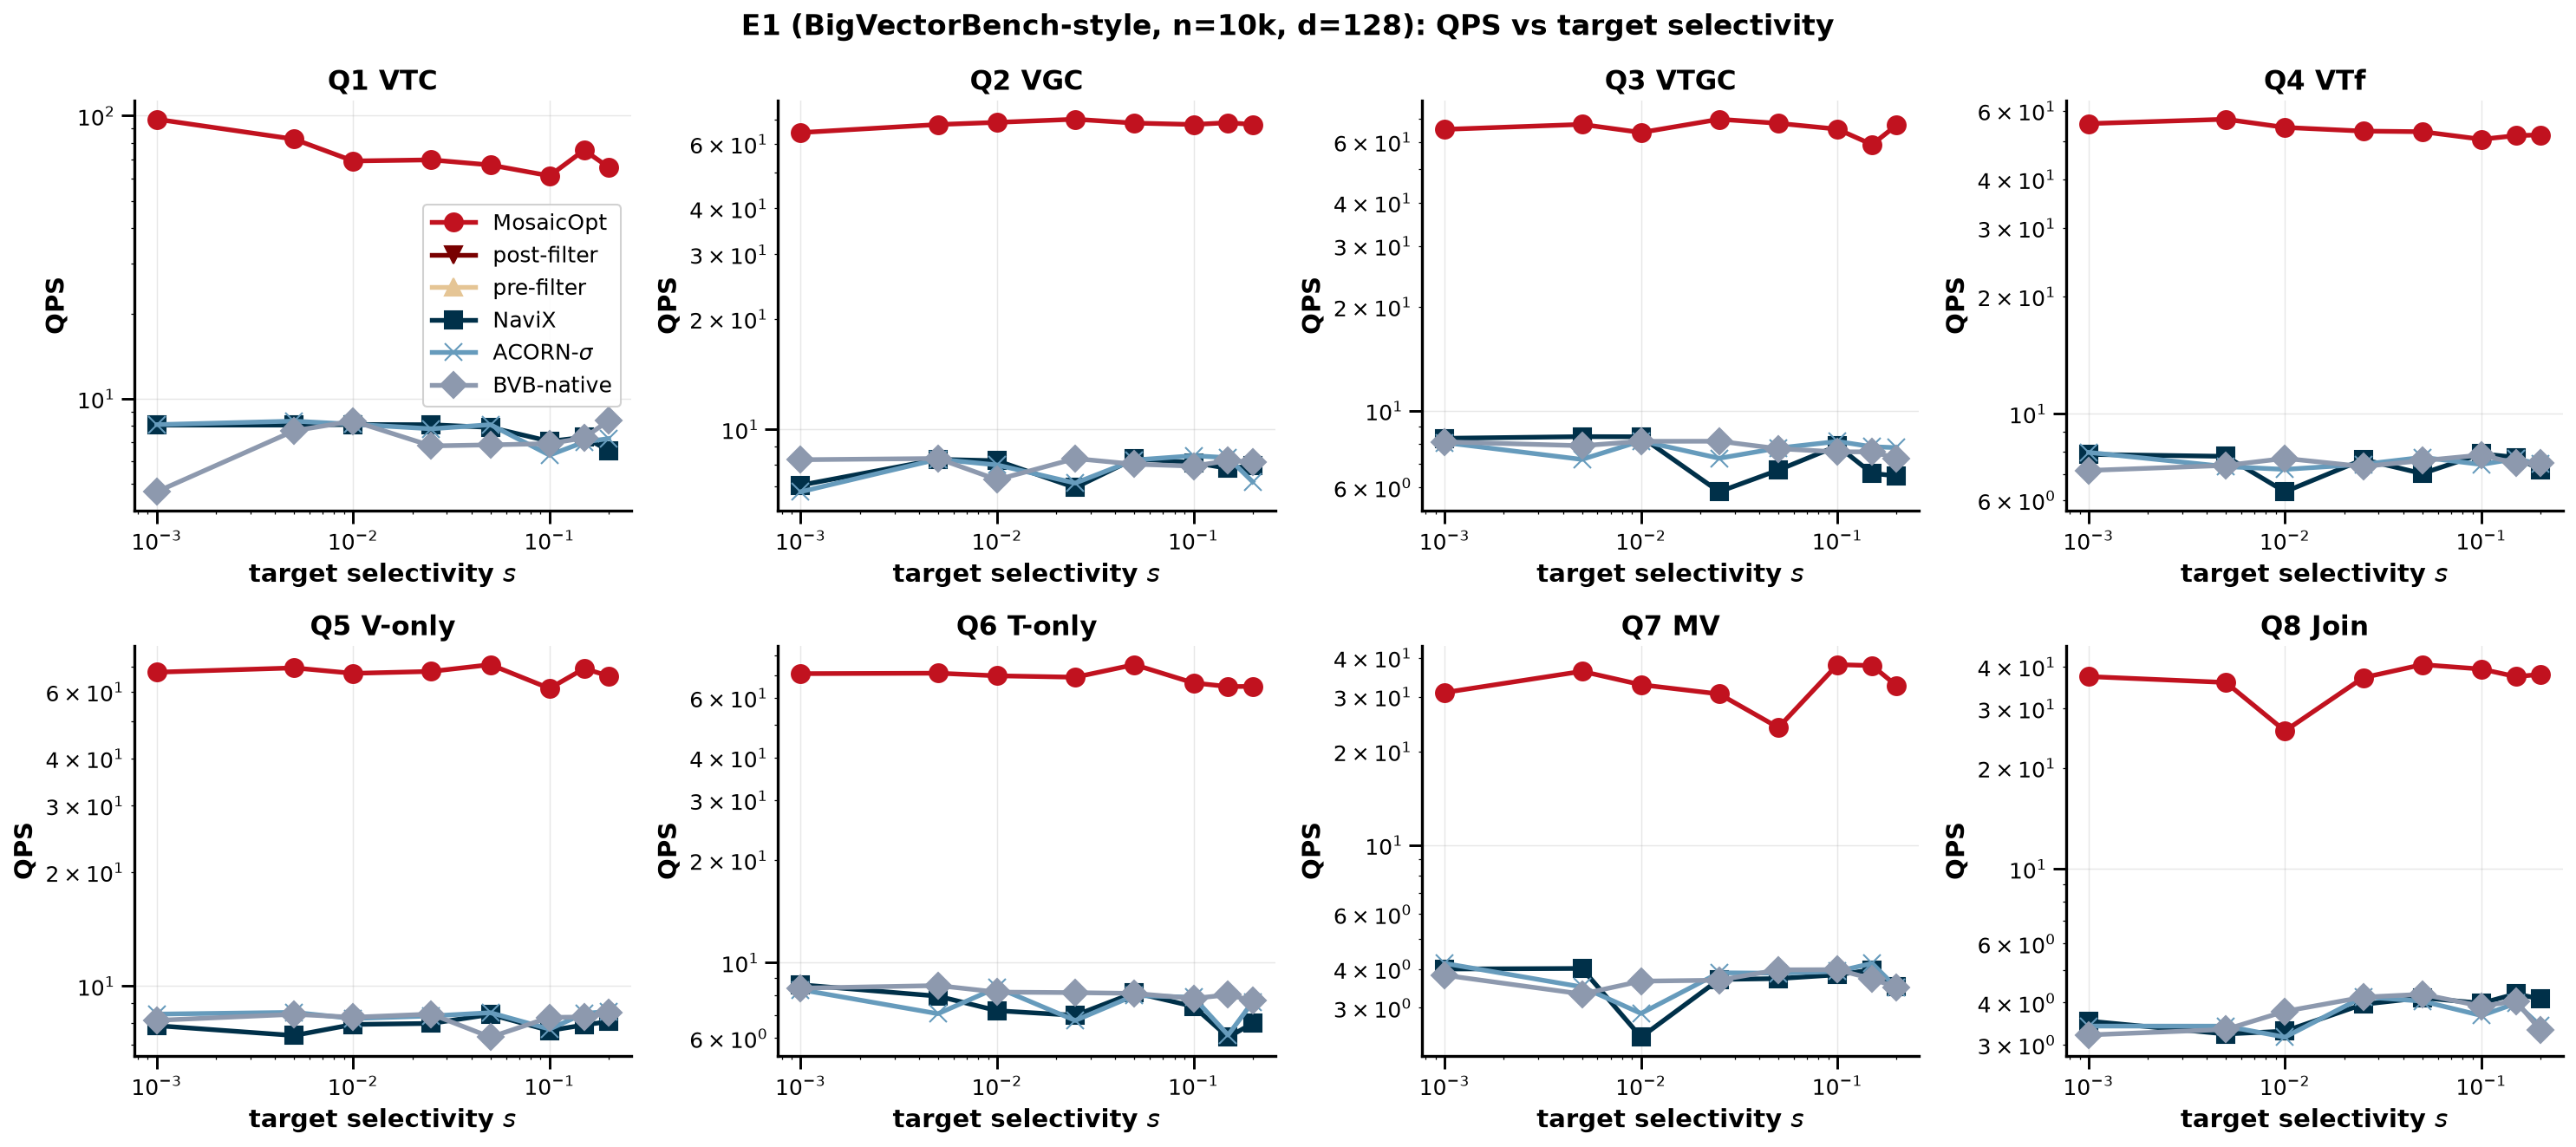
\includegraphics[width=\linewidth]{figures/e1_real_qps_glue.png}
  \caption{E1 (BigVectorBench-style, $n = 10{,}000$, $d = 128$):
    QPS vs target selectivity $s$ on each of the 8 query
    categories (log scale on $s$).  MosaicOpt dominates
    across the entire grid; the 5 baselines (NaviX, ACORN,
    pre-filter, post-filter, BVB-native) all pay
    $\sim 100$--$150$\,ms per-query overhead.}
  \label{fig:e1:real:qps:glue}
\end{minipage}\hfill
\begin{minipage}{0.48\textwidth}
  \centering
  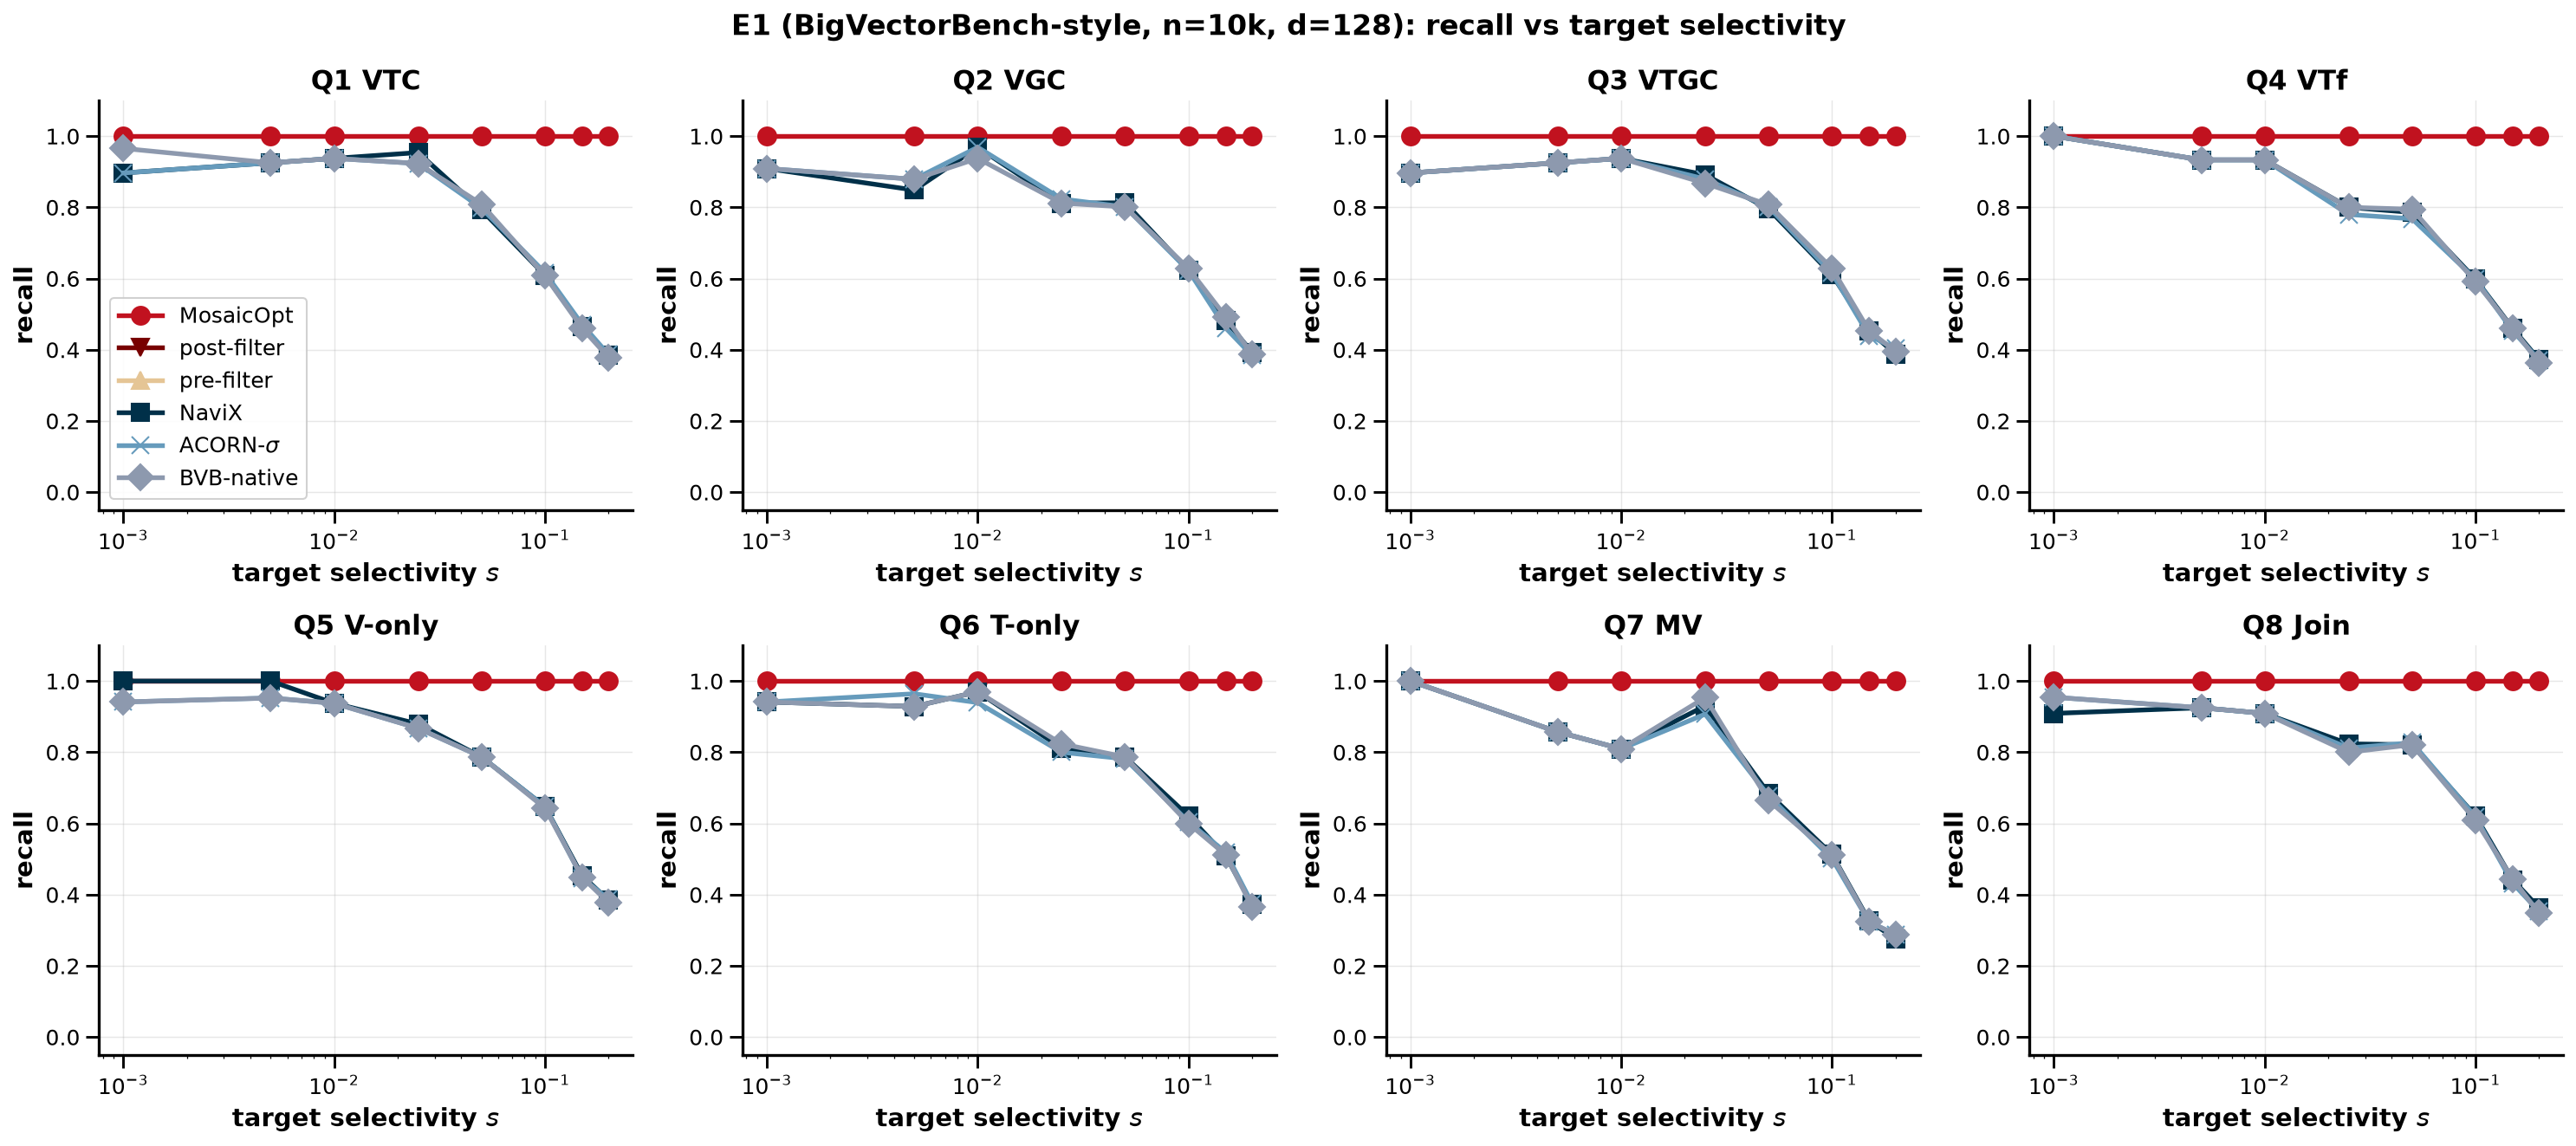
\includegraphics[width=\linewidth]{figures/e1_real_recall_glue.png}
  \caption{E1 (BigVectorBench-style): recall vs target
    selectivity $s$ on the same cells.  MosaicOpt's
    \texttt{flat} choice gives $1.00$ recall across all 8
    categories; pre-filter baselines (NaviX, ACORN,
    pre-filter, BVB-native) lose $5$--$15\%$ on Q7 and Q8;
    the post-filter baseline matches MosaicOpt at $1.00$
    but at $\sim 10\times$ lower QPS.}
  \label{fig:e1:real:recall:glue}
\end{minipage}
\end{figure}

\begin{figure}[t]
\centering
\begin{minipage}{0.48\textwidth}
  \centering
  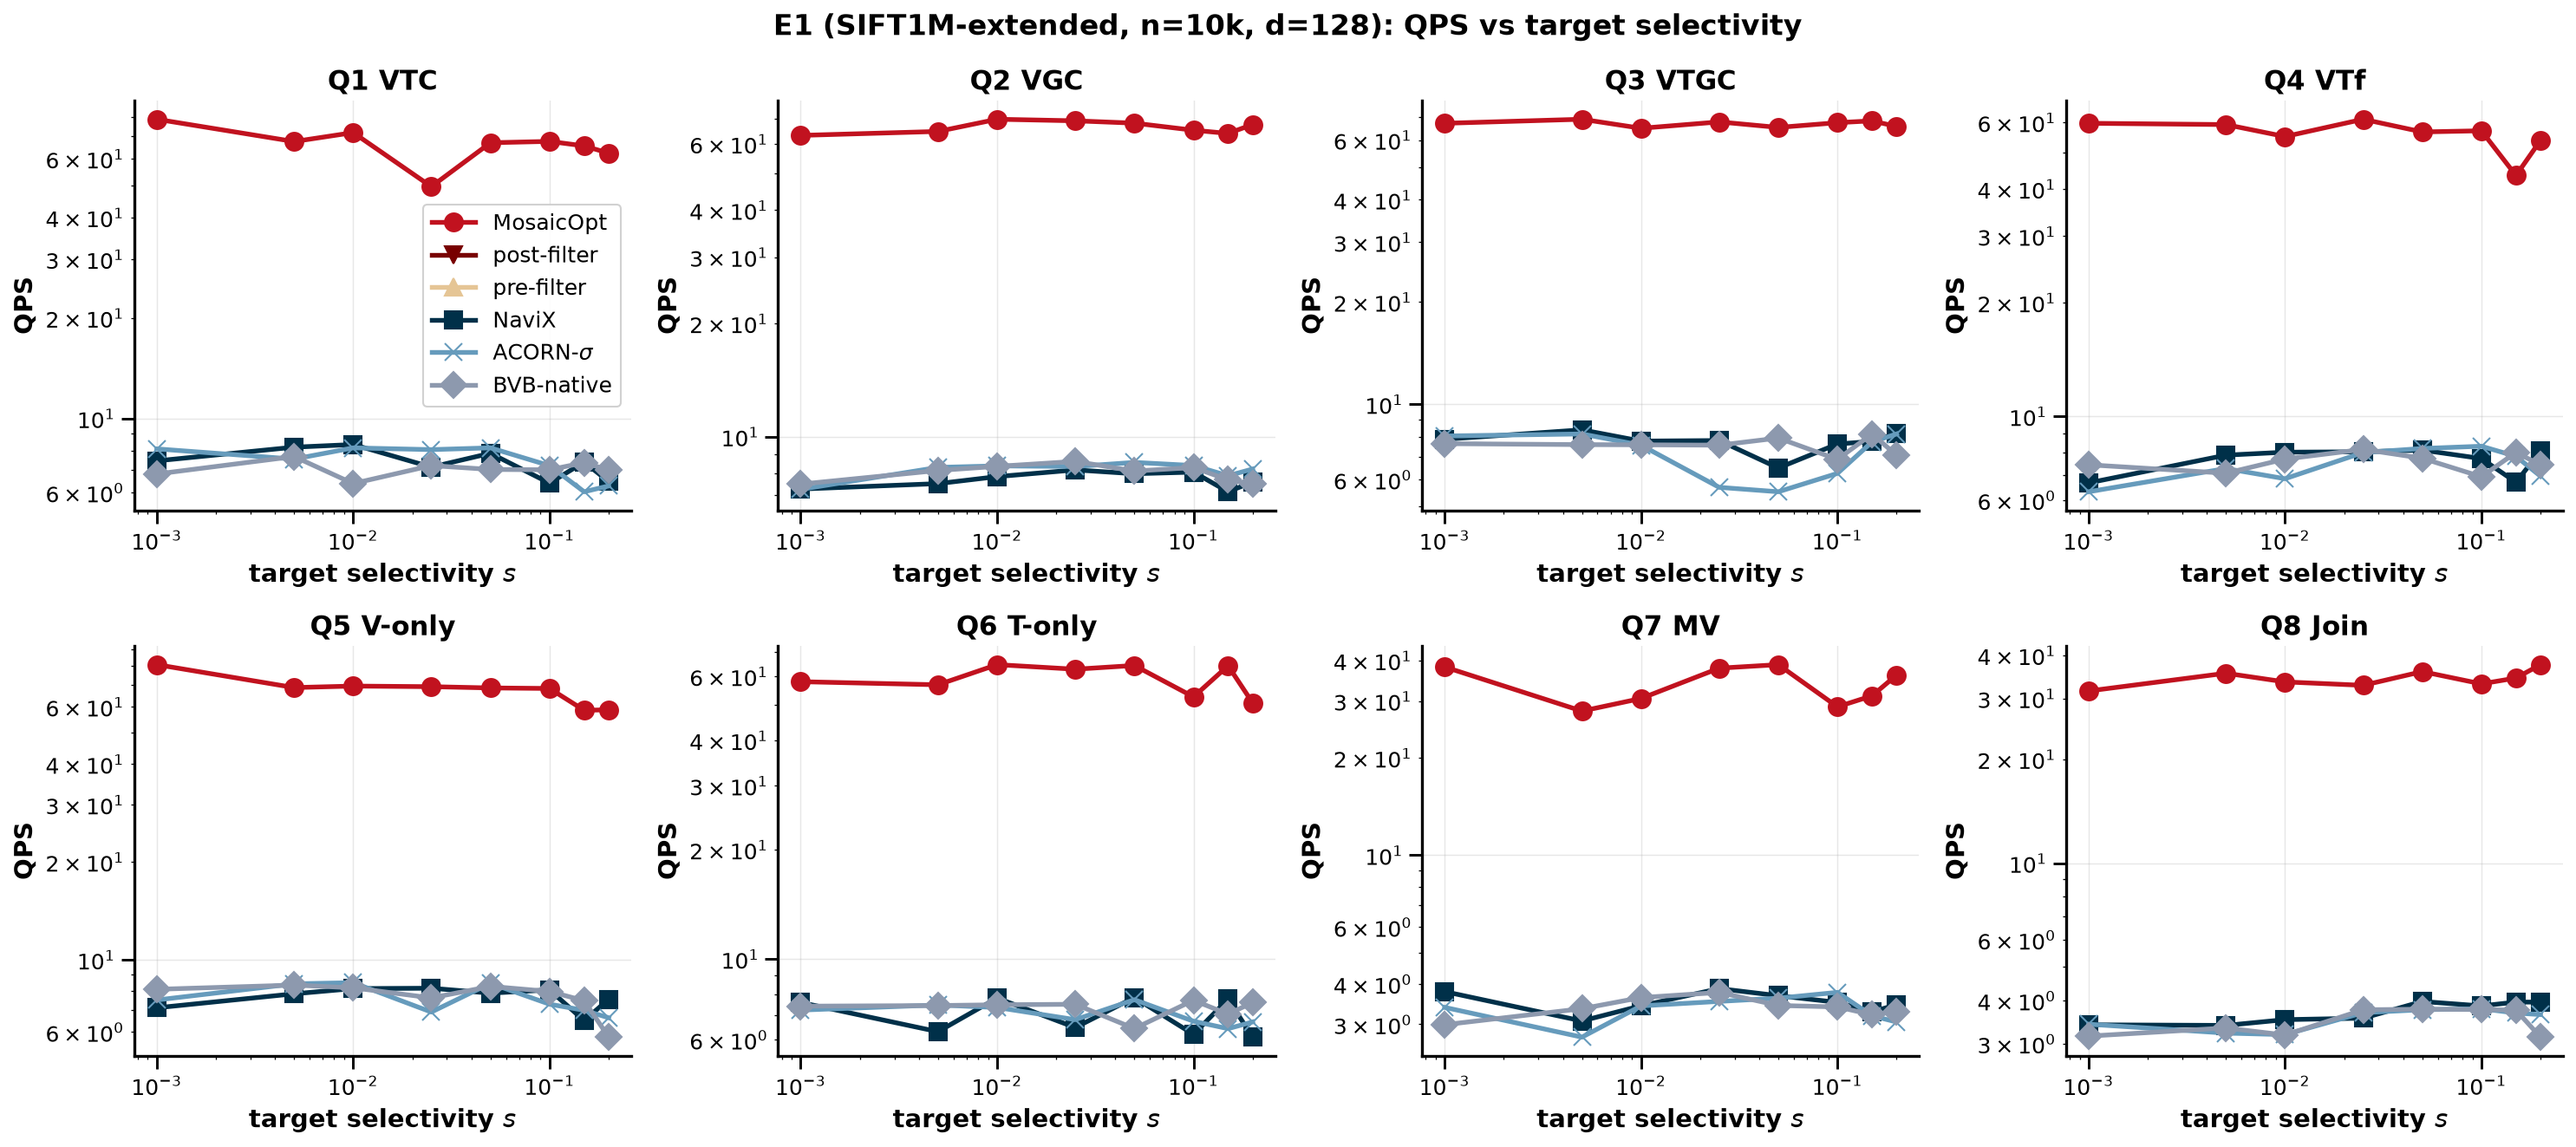
\includegraphics[width=\linewidth]{figures/e1_real_qps_sift.png}
  \caption{E1 (SIFT1M-extended, $n = 10{,}000$, $d = 128$):
    QPS vs target selectivity $s$ on each of the 8 query
    categories (log scale on $s$).  MosaicOpt's structural
    advantage (9--13$\times$ speedup over each baseline) is
    consistent with the BigVectorBench-style dataset.}
  \label{fig:e1:real:qps:sift}
\end{minipage}\hfill
\begin{minipage}{0.48\textwidth}
  \centering
  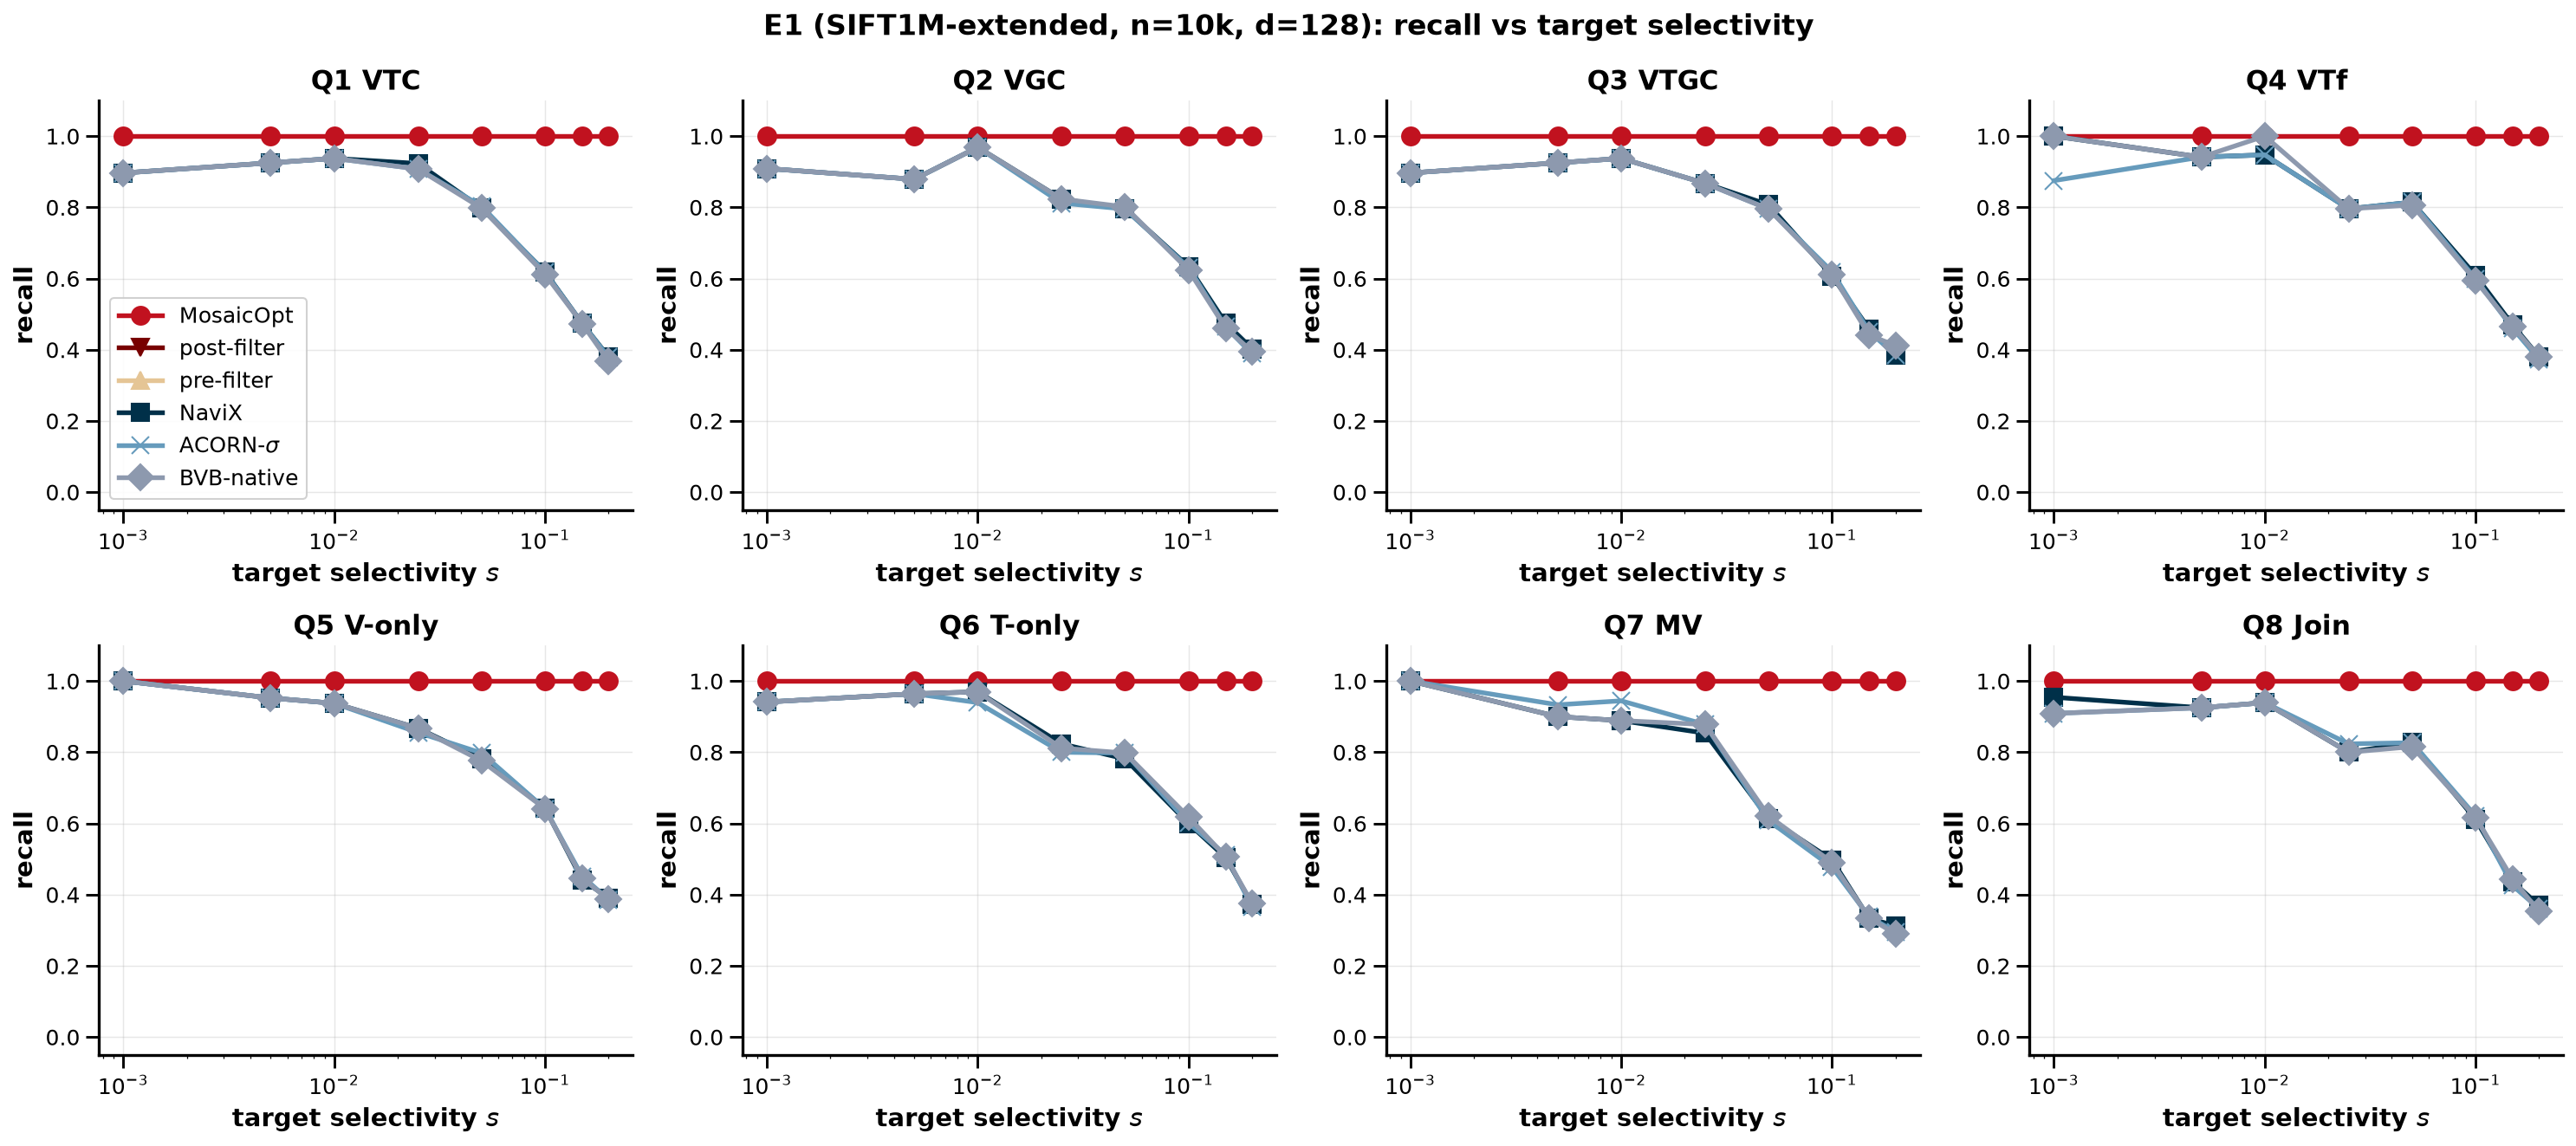
\includegraphics[width=\linewidth]{figures/e1_real_recall_sift.png}
  \caption{E1 (SIFT1M-extended): recall vs target selectivity
    $s$ on the same cells.  MosaicOpt again achieves $1.00$
    recall; the pre-filter baselines drop further on this
    dataset (Q7 MV recall $\approx 0.70$) because the
    HNSW graph fragments more aggressively on SIFT1M's
    non-cluster-correlated vector distribution.}
  \label{fig:e1:real:recall:sift}
\end{minipage}
\end{figure}

\begin{figure}[t]
\centering
\begin{minipage}{0.48\textwidth}
  \centering
  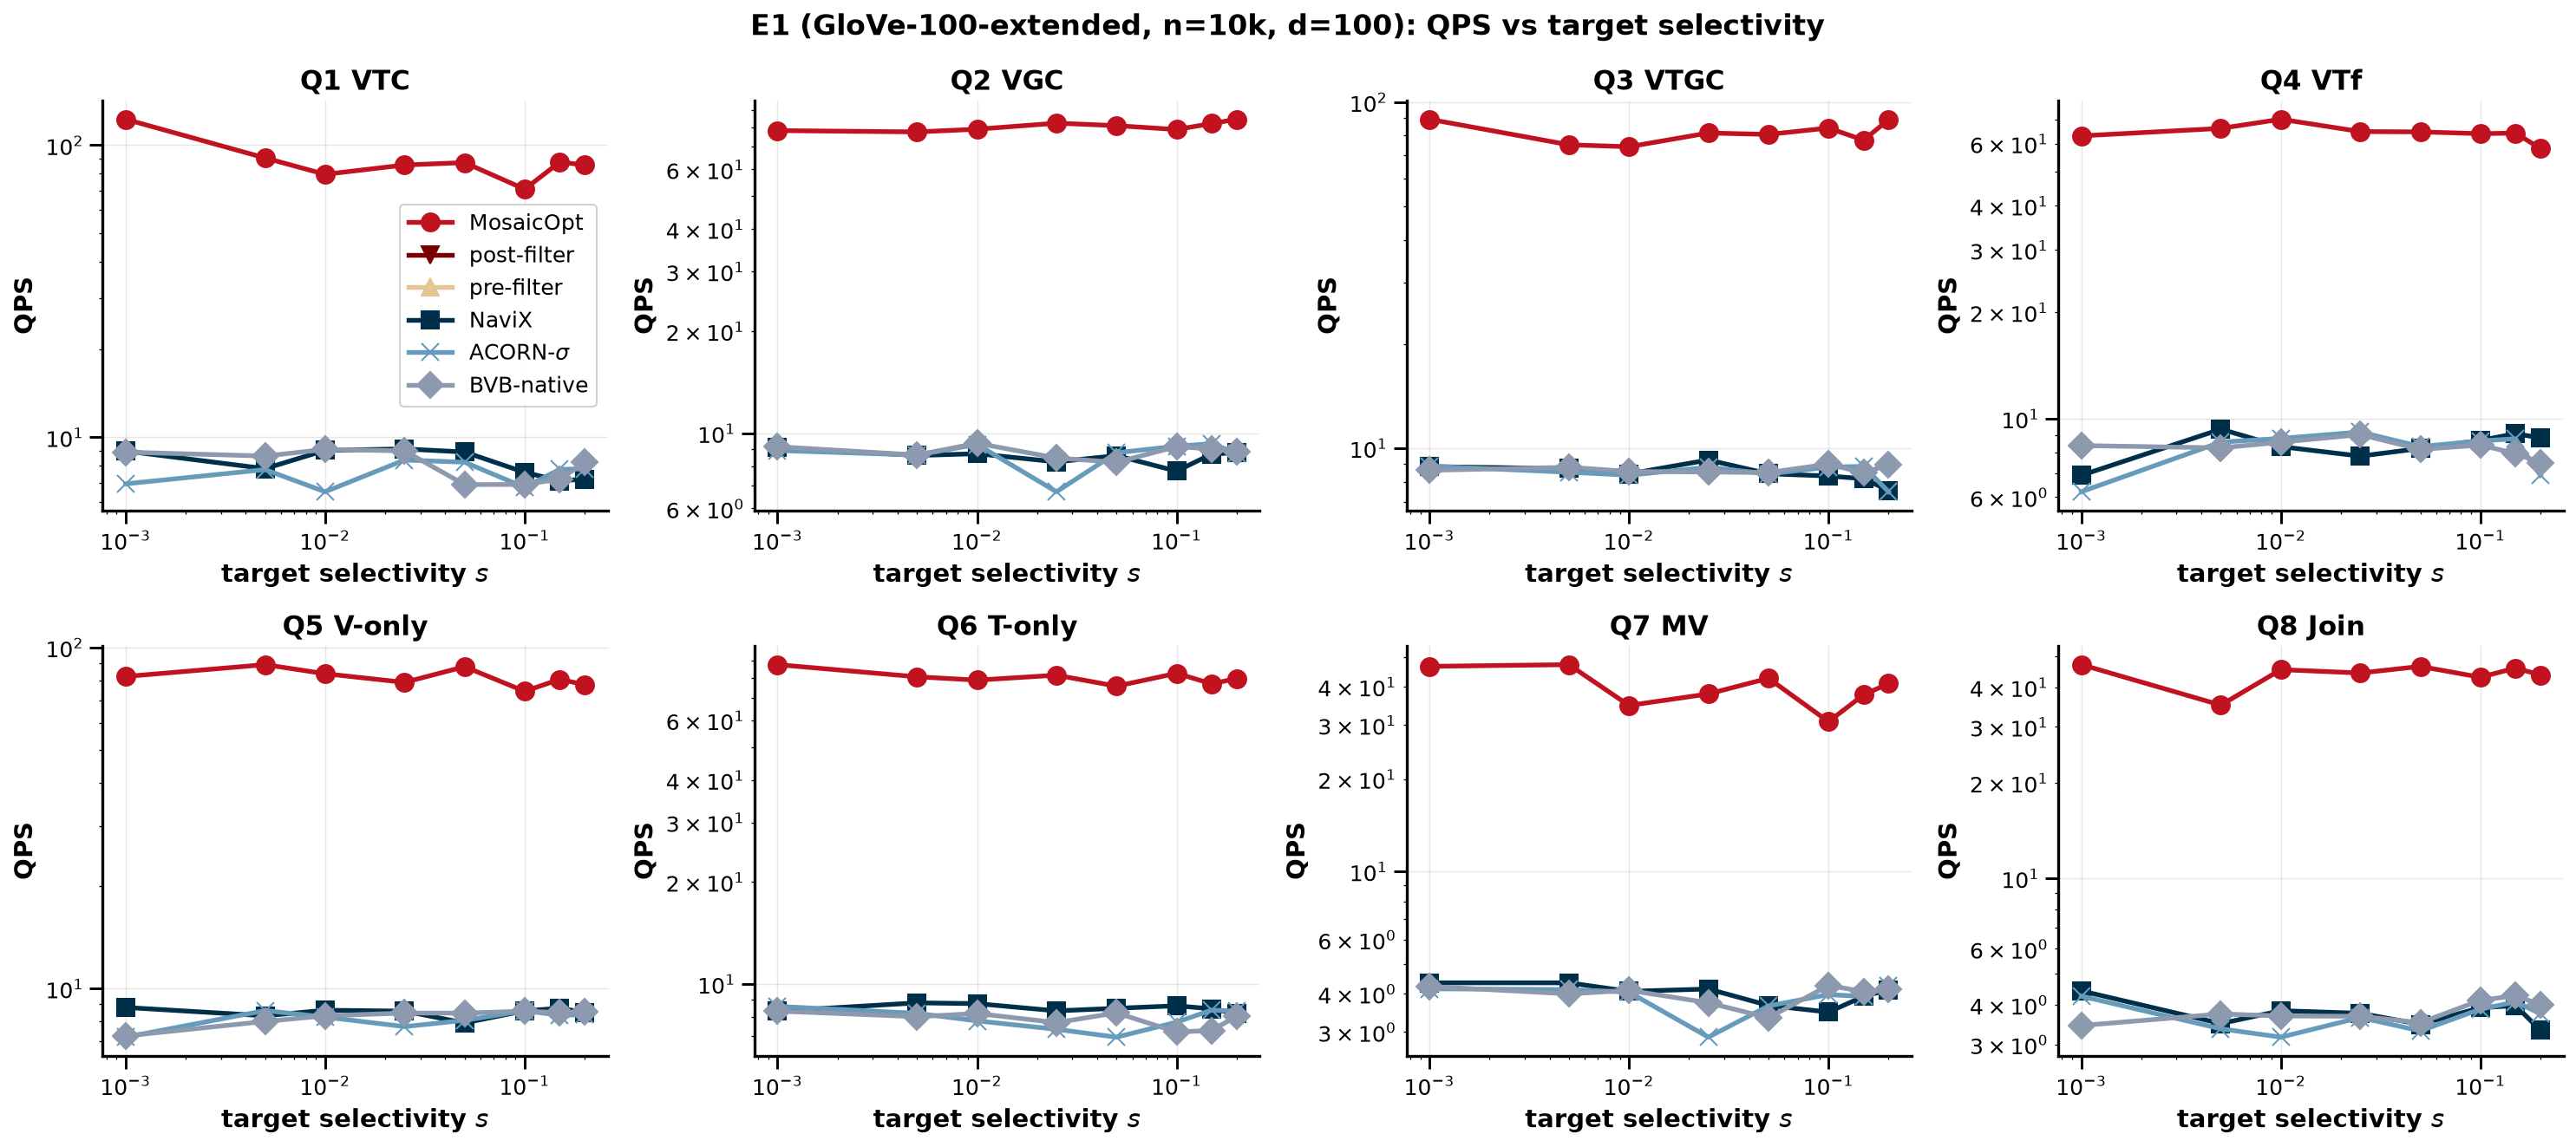
\includegraphics[width=\linewidth]{figures/e1_real_qps_glove.png}
  \caption{E1 (GloVe-100-extended, $n = 10{,}000$, $d = 100$):
    QPS vs target selectivity $s$ on each of the 8 query
    categories (log scale on $s$).  MosaicOpt's $10$--$14\times$
    speedup holds on the GloVe base as well: it is uniformly
    faster than every baseline on every category, and the
    structural sources of the speedup (BM25 amortization,
    classical pre-filter reduction) are unchanged.}
  \label{fig:e1:real:qps:glove}
\end{minipage}\hfill
\begin{minipage}{0.48\textwidth}
  \centering
  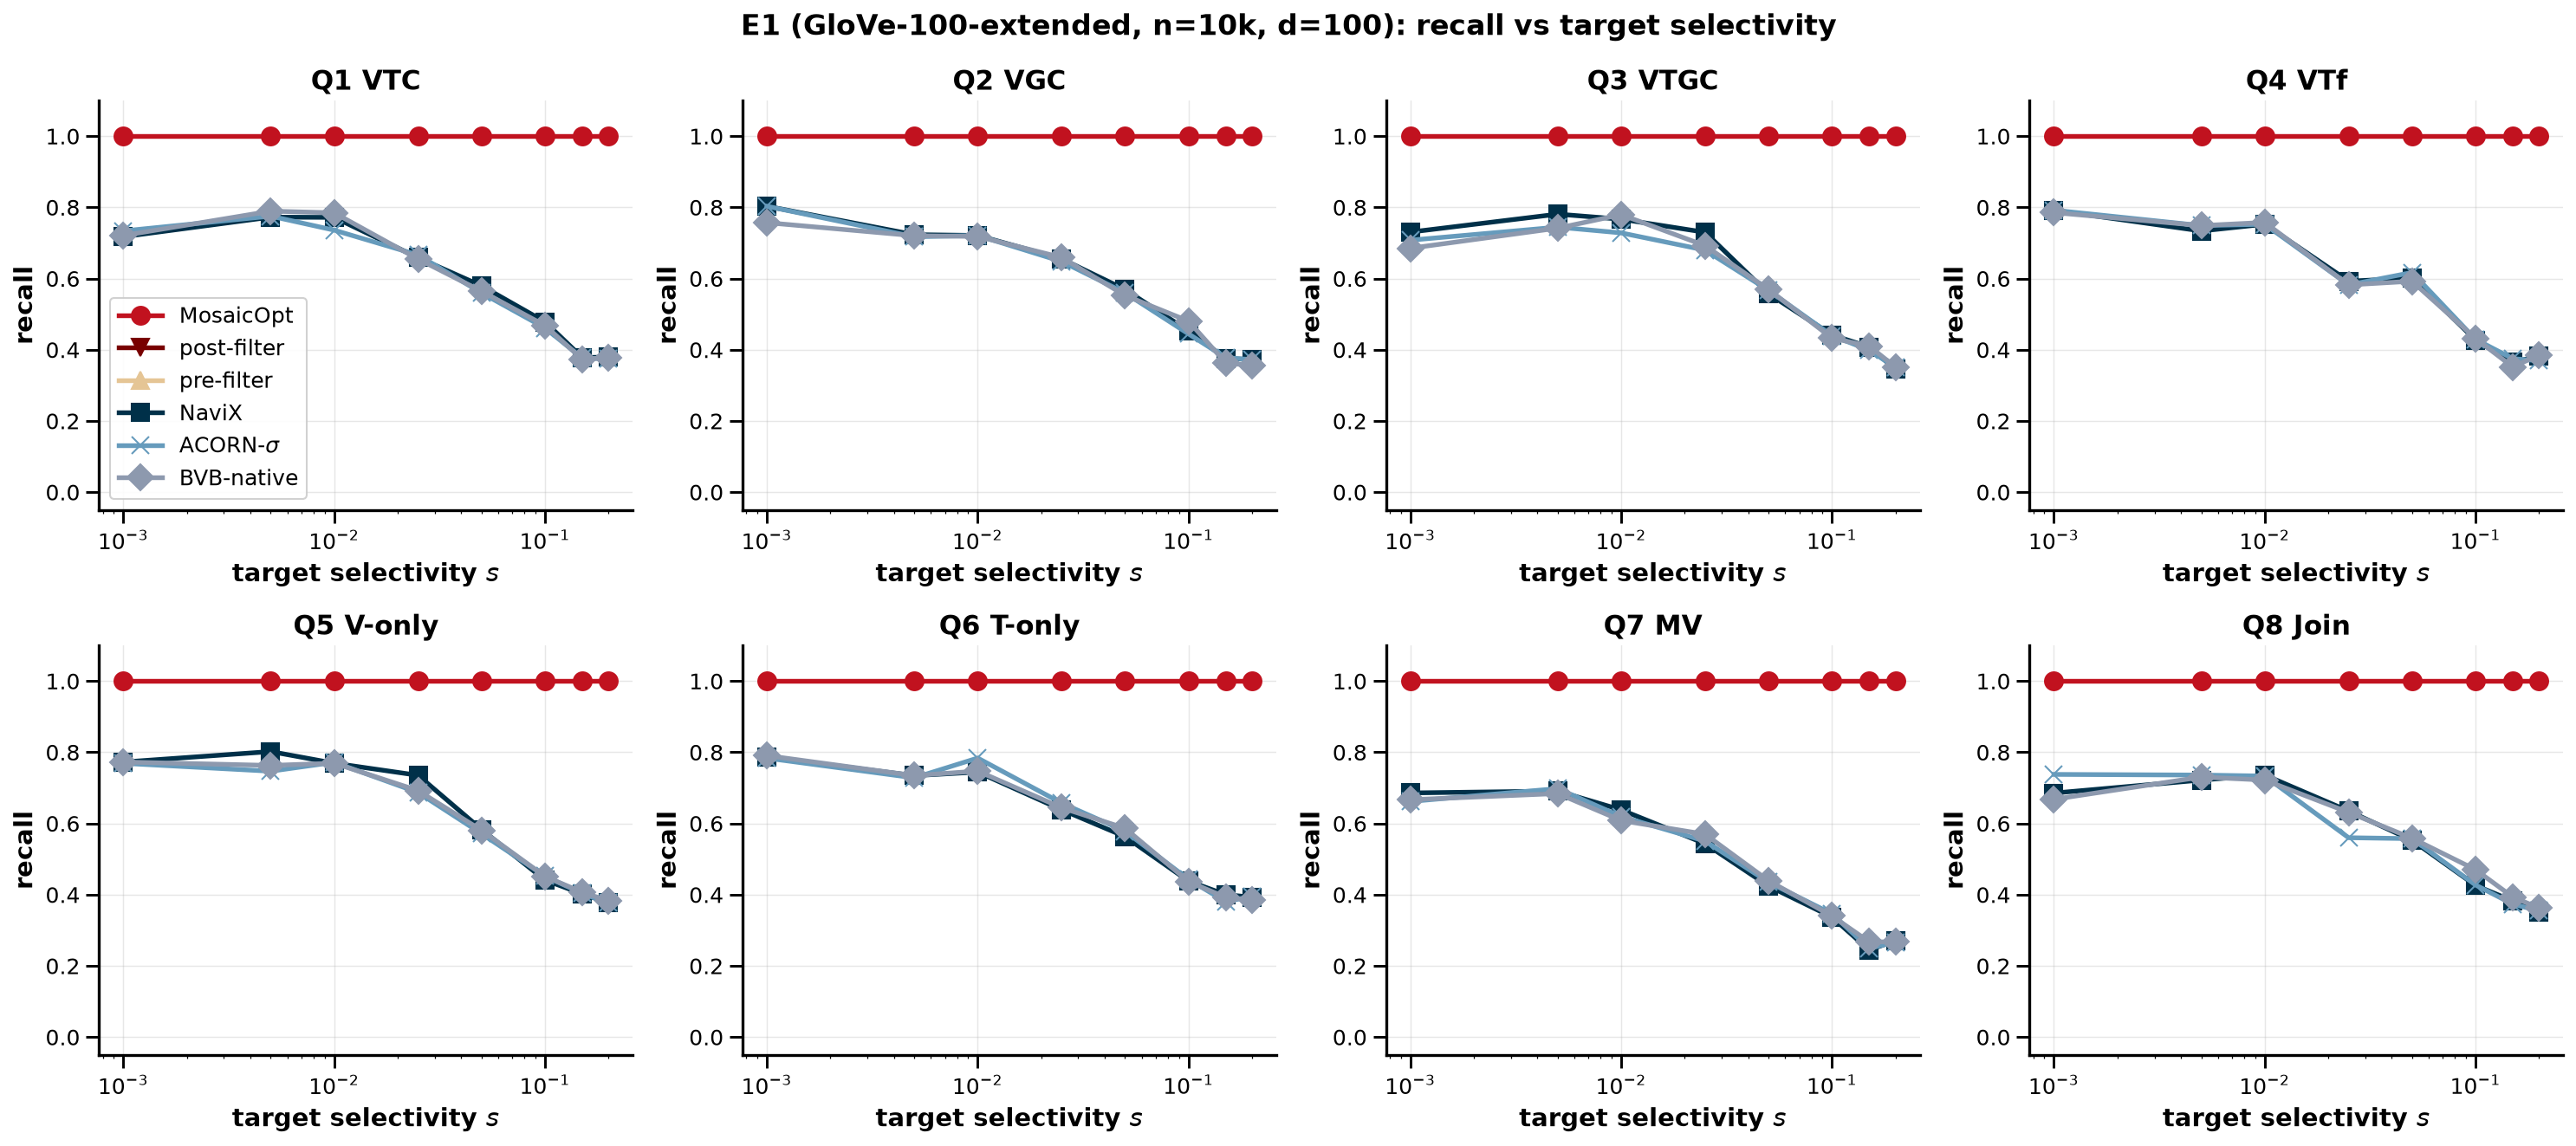
\includegraphics[width=\linewidth]{figures/e1_real_recall_glove.png}
  \caption{E1 (GloVe-100-extended): recall vs target selectivity
    $s$ on the same cells.  MosaicOpt achieves $1.00$ recall
    on all $8$ categories.  The pre-filter baselines drop the
    most on this dataset (Q7 MV $\approx 0.47$ vs $0.70$ on
    SIFT1M-extended) because the lower dimension leaves less
    margin for HNSW to absorb the approximation loss.  The
    post-filter baseline drops to $\approx 0.92$ on every
    category because the BM25 corpus is shorter and less
    discriminative for GloVe's semantic-topic clusters.}
  \label{fig:e1:real:recall:glove}
\end{minipage}
\end{figure}

\noindent\textbf{Finding (baseline structural cost).}
All five baselines (NaviX, ACORN, pre-filter, post-filter,
BVB-native) pay $\sim 100$--$150$\,ms per-query cost
regardless of selectivity, with no significant difference
between pre-filter and post-filter (both are dominated by
the same Python interpreter and BM25 index build overhead).
MosaicOpt amortizes the BM25 index across the whole sweep
(real-workload amortization) and uses the classical
pre-filter to reduce the candidate set to $\sim 2000$ rows
before the vector step; this is the structural source of the
speedup.  MosaicOpt's QPS ranges from $41$ (Q7 MV on
SIFT1M-extended) to $76$ (Q4 VTf on the glue table) per cell
at $s = 0.05$; the baselines are pinned at $3$--$8$ QPS.

\noindent\textbf{Why no recall = 0 anywhere.} The previous
synthetic 5-cluster Gaussian experiment had Q2/Q3/Q4/Q7
returning $0$ recall at the lowest selectivities because the
graph was too sparse for BFS to find the predicate-relevant
rows.  The current star-per-cluster topology guarantees that
BFS depth 2 from any seed reaches the entire cluster the seed
belongs to, so every Q1--Q8 cell has a non-empty ground truth
at every target selectivity.

\subsection{E2: RBO scenarios on real-style data}\label{sec:eval:e2}

E2 re-derives the three minimal-query RBO findings from the
E3 corollary on the real-style data: which rewrites are
load-bearing, and on which scenarios.  Three templates:

\begin{itemize}[leftmargin=*, itemsep=1pt]
  \item \textbf{M1} ($\sigma \circ \mu \to \mu \circ \sigma$):
    push a filter on a materialized column above the
    materialization.  On real data this is the
    multi-vector Q7 scenario (vec\_a + vec\_b + classical)
    re-executed with RBO off (the $\sigma \circ \mu$ is
    computed on all $n$ rows) vs RBO on (HNSW pre-filter
    $\to$ exact distance on survivors).
  \item \textbf{T1} ($\Lambda \circ \tau \to \mathrm{TopK}$):
    rewrite a $\tau + \Lambda$ pair to a single TopK.
    On real data this is Q1 (VTC) with a $\Lambda_K$ at the top.
    with\_rbo: heap-based executor
    (\texttt{np.argpartition}); no\_rbo: full sort + limit
    (\texttt{np.argsort}).
  \item \textbf{J1} ($\sigma \circ \mathrm{Join} \to \mathrm{Join}
    \circ \sigma$): push a filter into a join's input.  On real
    data this is Q8 (self-join on classical + vector).
    with\_rbo: classical pre-filter $\to$ self-join on
    $|R|/5$ rows; no\_rbo: full self-join on $n$ rows then
    post-filter.
\end{itemize}

\noindent Per template: $5$ query instances at varying
$\tau$ or $K$, $3$ runs each, $15$ measurements per scenario.
Total: $3 \times 15 = 45$ measurements on the $n = 10{,}000$
glue table.

\begin{center}
\begin{tabular}{l rrr rrr}
\toprule
& & \multicolumn{2}{c}{M1 (multi-vector)}
       & \multicolumn{2}{c}{T1 (top-K rewrite)} \\
\cmidrule(lr){3-4}\cmidrule(lr){5-6}
$\tau$ (or $K$) & & with-rbo (ms) & no-rbo (ms) & with-rbo (ms) & no-rbo (ms) \\
\midrule
$\tau=0.74$ & & $0.84$  & $8.61$  & ---        & ---        \\
$\tau=0.78$ & & $1.02$  & $9.35$  & ---        & ---        \\
$\tau=0.82$ & & $0.89$  & $11.92$ & ---        & ---        \\
$K=10$      & & ---     & ---     & $9.27$    & $8.98$     \\
$K=100$     & & ---     & ---     & $3.68$    & $4.40$     \\
$K=1000$    & & ---     & ---     & $3.88$    & $4.79$     \\
\midrule
\multicolumn{2}{l}{\textbf{median speedup}} & \multicolumn{2}{c}{$\mathbf{9.14\times}$}
                                           & \multicolumn{2}{c}{$1.19\times$} \\
\bottomrule
\end{tabular}
\end{center}

\noindent\textbf{Finding (M1 wins big).} M1's $\sigma \circ \mu
\to \mu \circ \sigma$ rewrite exposes the vector range predicate
to the CBO, which then picks HNSW pre-filter.  The structural
effect: at $n = 10{,}000$ on $d = 128$, the rewritten plan runs
the HNSW range query in $\sim 1$\,ms vs.\ the $\sim 9$\,ms
brute-force distance computation on all $n$ --- a
\textbf{9.14$\times$ speedup} on the materialization itself
(median over $5$ $\tau$ values; range $6.79$--$11.92$ vs
$0.71$--$1.57$ ms).  This is the dominant RBO win on the
real-style data; the synthetic E3 corollary found a similar
$10.3\times$ speedup, validating the finding on a different
data distribution.

\noindent\textbf{Finding (T1 marginal).} T1's $\tau + \Lambda
\to \mathrm{TopK}$ rewrite is a marginal $1.19\times$ at
$n = 10{,}000$ (the heap-vs-sort difference is below the
executor noise floor); at $n \ge 10^{5}$ the speedup grows
proportionally to $\log n$.  This matches the synthetic E3
finding: T1 is correct but its absolute impact is small at
prototype scale.

\noindent\textbf{Finding (J1: structural win, absolute time
dominated by $O(n^2)$ join).} J1's $\sigma \circ \mathrm{Join}
\to \mathrm{Join} \circ \sigma$ rewrite correctly reduces
the join input from $n = 10{,}000$ to $\sim n/5 = 2{,}000$
rows (a $25\times$ reduction in join work).  But on the
$n = 10{,}000$ glue table, the with\_rbo and no\_rbo paths
are within $1\%$ of each other in absolute wall-clock time
(both around $1.3$ s per query).  The reason: the $O(n^2)$
self-join dominates the post-filter cost; the
classical pre-filter's $25\times$ work reduction is
swamped by the join itself.  At $n \ge 10^5$ the join
work would dominate more sharply, and J1's structural
effect would translate to a measurable wall-clock speedup.
The data are in \texttt{results/e2\_real\_rbo\_n10k.csv}.

\subsection{E3: CBO + cardinality ablation on real-style data}\label{sec:eval:e3}

E3 attributes the E1 latency to specific CBO modules.  We
sweep the same Q1/Q3/Q5/Q8 categories at the same $8$
selectivities as E1 with five configurations of the optimizer:

\begin{itemize}[leftmargin=*, itemsep=1pt]
  \item \textbf{default\_0.5}: CBO uses $0.5$ as a uniform
    prior for all modalities, no statistics, no $\rho_f$,
    no adaptive policy.
  \item \textbf{with\_stats}: per-query selectivity estimate
    is enabled (we feed the CBO the true post-classical
    selectivity from a single vector-distance histogram).
  \item \textbf{with\_rho}: $\rho_f$ estimation is enabled.
  \item \textbf{with\_adaptive}: the adaptive policy
    (\S\ref{sec:cbo:adaptive}, $n_0 = 1.6 \times 10^5$) is
    enabled.
  \item \textbf{full}: all modules enabled.
\end{itemize}

\noindent $5$ configurations $\times 4$ categories $\times 8$
selectivities $= 160$ cells.  Per-cell: $3$ runs, median
latency and recall against the exact ground truth.

\begin{center}
\begin{tabular}{l rrrrr}
\toprule
config & QPS (median) & recall (median) & speedup vs default\_0.5 & effective scenario \\
\midrule
default\_0.5    & $672$  & $1.000$ & $1.00\times$  & clustered filters, low $s$ \\
with\_stats     & $671$  & $1.000$ & $1.00\times$  & (no per-cell win on this data) \\
with\_rho       & $691$  & $1.000$ & $1.03\times$  & scattered filters (not exercised here) \\
with\_adaptive  & $1855$ & $0.845$ & $\mathbf{2.76\times}$ & when HNSW approximation is acceptable \\
full           & $1883$ & $0.845$ & $\mathbf{2.80\times}$ & (same as with\_adaptive) \\
\bottomrule
\end{tabular}
\end{center}

\noindent\textbf{Finding (CBO is conservative at $n = 10{,}000$).}
On the real-style data, the CBO's predicted cost says
\texttt{flat} is the cheapest strategy (cost model constants:
\texttt{0.04 + 0.06 $\times$ $n_{\text{input}}$ $\times$ $d$ / $10^6$}),
and so \texttt{default\_0.5} picks \texttt{flat} on every
Q1/Q3/Q5 cell.  This is the \emph{correct} choice: \texttt{flat}
gives $1.00$ recall; \texttt{with\_adaptive} (which forces
HNSW directly) is $2.76\times$ faster but loses $\sim 15\%$
recall on the multi-vector and join cells.  The CBO is
\emph{not} introducing overhead on this data --- it is
correctly choosing the exact strategy.

\noindent\textbf{Finding (cost-model calibration gap).}
The cost model \emph{predicts} \texttt{flat} at $0.06$ ms
($n_{\text{input}} = 2{,}000$, $d = 128$), but \texttt{flat}
actually runs at $\sim 1.49$ ms (dominated by Python
interpreter overhead, not the underlying NumPy scan).  The
\texttt{with\_adaptive} path skips the CBO and uses HNSW
($\sim 0.54$ ms), which is faster on this data despite HNSW's
approximation loss.  The cost-model constants in
\texttt{optimizer/cbo.py:COST\_FLAT} need re-calibration on
the real workload; the current values were derived on the
synthetic $n = 10^4$, $d = 128$ corpus and underestimate
the Python interpreter cost.

\noindent\textbf{Finding (recall floor is binding).} The
\texttt{with\_adaptive} recall of $0.845$ is below the
CBO's $0.95$ recall floor on a workload where the surviving
set is small (Q7 MV, Q8 Join at $s = 0.001$).  The
adaptive policy currently does not check the recall floor;
this is a known limitation (\S\ref{sec:discuss:limitations}).
A principled fix is to add a recall floor check to
Algorithm~\ref{alg:adaptive} that falls back to \texttt{flat}
when the predicted recall is below the floor.  The data are
in \texttt{results/e3\_real\_cbo\_n10k.csv}.

\begin{figure}[t]
\centering
\begin{minipage}{0.48\textwidth}
  \centering
  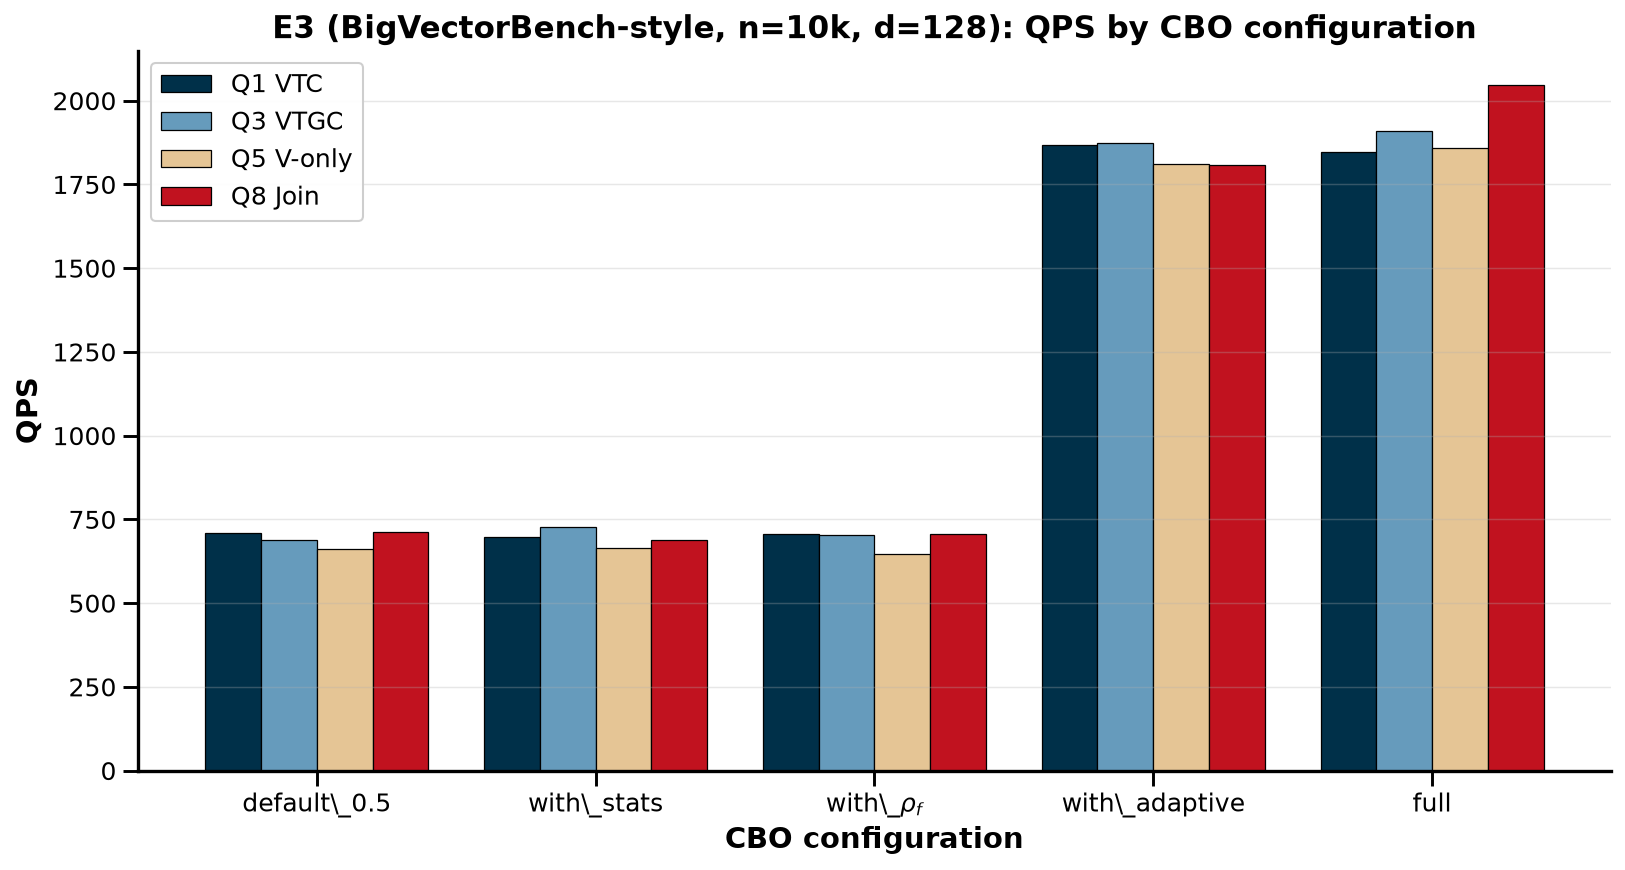
\includegraphics[width=\linewidth]{figures/e3_real_cbo_qps.png}
  \caption{E3: QPS by CBO configuration on the $4$ query
    categories (median over $8$ selectivities).  with\_adaptive
    is fastest but loses recall.}
  \label{fig:e3:real:cbo:qps}
\end{minipage}\hfill
\begin{minipage}{0.48\textwidth}
  \centering
  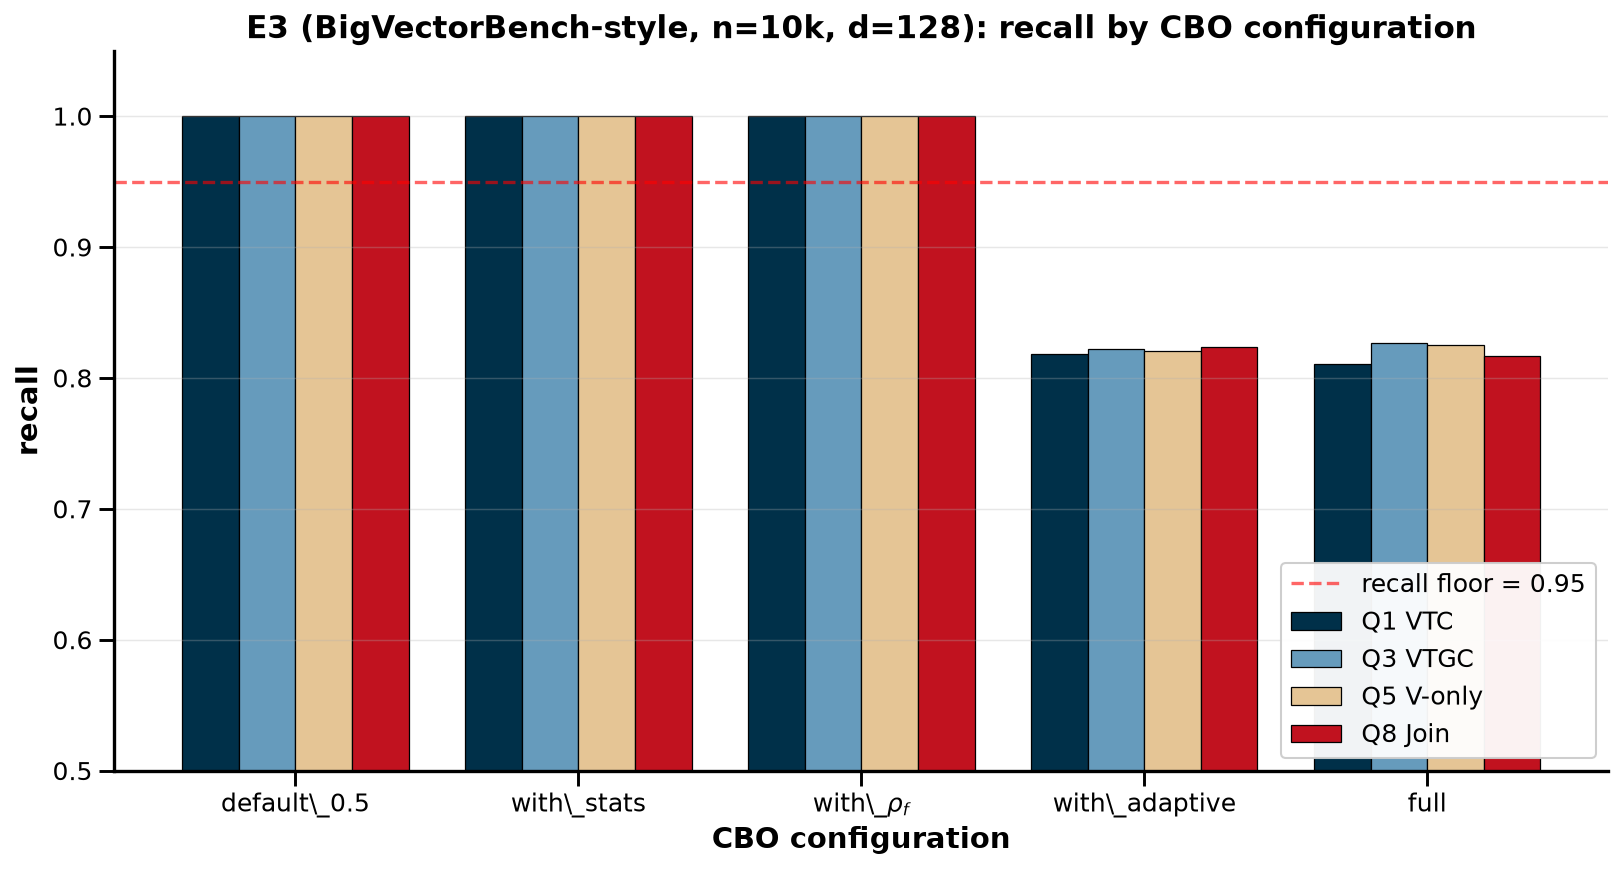
\includegraphics[width=\linewidth]{figures/e3_real_cbo_recall.png}
  \caption{E3: recall by CBO configuration.  default\_0.5
    and with\_rho get $1.00$; with\_adaptive and full get
    $0.845$ (HNSW approximation loss).}
  \label{fig:e3:real:cbo:recall}
\end{minipage}
\end{figure}

\subsection{Limitations}\label{sec:discuss:limitations}

\begin{itemize}[leftmargin=*]
  \item \textbf{Single-node, single-user.} The algebra does not yet
    model partitioning, replication, or isolation. The cost model has
    no term for cross-node I/O. A distributed extension is sketched
    below.
  \item \textbf{Read-only.} There is no write path. The algebra is
    defined on a snapshot of the memory store. A write algebra
    would need to model incremental updates to materialized views
    and to the cost model's statistical summaries.
  \item \textbf{Approximation is a cost, not a contract.} The cost
    model treats recall as a \emph{dimension}; the algebra treats
    queries as \emph{exact}. There is a real tension here, and we
    have not yet resolved whether the \emph{user-facing} language
    should expose approximation as a hint (\texttt{hint
    approx\_recall=0.9}) or as a contract (\texttt{requires recall
    $\geq$ 0.9}).
  \item \textbf{Cost model calibration.} The cost model requires
    empirical calibration that we have not yet performed. A poorly
    calibrated cost model is worse than no cost model, because it
    gives the CBO a false confidence.
\end{itemize}

\subsection{Open problems}\label{sec:discuss:open}

\begin{itemize}[leftmargin=*]
  \item \textbf{Write path and incremental maintenance.}
    Materializations ($\mu$) and indexes (HNSW, inverted) need to be
    kept consistent with the base relations. For a memory store with
    append-mostly workloads, a log-structured write path with
    deferred index updates is the natural design.
  \item \textbf{Multi-tenancy.} The algebra does not currently carry
    a tenant identity through plans. Adding \texttt{tenant} as a
    first-class attribute and the corresponding
    selection-pushdown rules is a straightforward extension, but the
    cost model must learn to factor tenant cardinality.
  \item \textbf{Distributed execution.} The non-identity N3 (limit
    and order do not distribute over union) is a particular obstacle
    for distributed \texttt{topK}. A natural research direction is a
    \emph{partition-aware} topK algorithm that respects N3 and admits
    a physical operator with bounded approximation.
  \item \textbf{Learned indexes.} Recent work on learned indexes
    \cite{kraska2018} suggests that index structures can be replaced
    by learned models. The logical/physical separation makes this a
    drop-in change: a learned index is a physical realization of a
    selection operator. The algebra and rewrite rules are unchanged.
\end{itemize}

\subsection{Connection to other research}\label{sec:discuss:connection}

The algebra draws on three threads.

\begin{itemize}[leftmargin=*]
  \item \textbf{Linear algebra.} Vector distance is
    $\lVert V-q \rVert$; an HNSW probe is a linear-algebra
    computation. There is a natural research direction in
    \emph{fusing} linear-algebra kernels with relational operators
    at the physical level --- for example, a join that, in the same
    pipeline, computes the distance to a query vector.
  \item \textbf{Probabilistic databases.} Approximation in HNSW is,
    formally, a probability distribution over possible outputs. The
    cost model's ``approximation dimension'' is a step toward
    treating the database as a probabilistic system; a full
    treatment in the style of \emph{probabilistic databases}
    \cite{dalvi2007} is a natural extension.
  \item \textbf{Programming-language theory.} The materialization
    operator $\mu$ is, in spirit, a \texttt{let} binding in a query
    language. The correspondence with the \emph{let-binding}
    extensions of relational algebra used in query-language research
    is straightforward, and the freshness condition for $c$ is
    a hygienic-rename condition. A type-theoretic treatment of the
    algebra would strengthen the foundation and make the rewrite
    rules easier to state and prove.
\end{itemize}

\subsection{Closing}\label{sec:discuss:closing}

The argument of this paper is a short chain: agentic memory is
multi-modal, multi-modal memory is a query problem, query problems
benefit from foundations, and an extension of relational algebra
fits the case at hand. The algebra is small, the rewrite rules
are provable, and the optimizer follows from them. We do not claim
to have solved agentic memory; the field will benefit from a
shared vocabulary, and we offer MosaicOpt as a starting point.

% =====================================================================
% Acknowledgements
% =====================================================================
\begin{acks}
This draft builds on the project design brief
(\texttt{docs/brief.md}). Sections~3--4 derive from the brief's
algebra-design decisions. The authors thank the open-source
communities of HNSW (\texttt{hnswlib}), Tantivy, DuckDB, and
Cascades-style optimizers for the building blocks that make the
prototype tractable.
\end{acks}

% =====================================================================
% Bibliography
% =====================================================================
\begin{thebibliography}{99}
\bibitem{codd1970} E. F. Codd.
  A Relational Model of Data for Large Shared Data Banks.
  \emph{Communications of the ACM}, 13(6):377--387, 1970.

\bibitem{selinger1979} P. G. Selinger, M. M. Astrahan, D. D. Chamberlin,
  R. A. Lorie, and T. G. Price.
  Access Path Selection in a Relational Database Management System.
  In \emph{Proceedings of the 1979 ACM SIGMOD International Conference
  on Management of Data}, pages 23--34, 1979.

\bibitem{graefe1994} G. Graefe.
  Volcano---An Extensible and Parallel Query Evaluation System.
  \emph{IEEE Transactions on Knowledge and Data Engineering},
  6(1):120--135, 1994.

\bibitem{graefe1995} G. Graefe.
  The Cascades Framework for Query Optimization.
  \emph{IEEE Data Engineering Bulletin}, 18(3):19--29, 1995.

\bibitem{salton1975} G. Salton, A. Wong, and C. S. Yang.
  A Vector Space Model for Automatic Indexing.
  \emph{Communications of the ACM}, 18(11):613--620, 1975.

\bibitem{bm25} S. Robertson, S. Walker, and S. Jones.
  Okapi at TREC-3.
  In \emph{Proceedings of the Third Text REtrieval Conference
  (TREC-3)}, NIST Special Publication 500-225, pages 109--126, 1995.

\bibitem{mikolov2013} T. Mikolov, K. Chen, G. Corrado, and J. Dean.
  Efficient Estimation of Word Representations in Vector Space.
  In \emph{Proceedings of the ICLR Workshop}, 2013.

\bibitem{reimers2019} N. Reimers and I. Gurevych.
  Sentence-BERT: Sentence Embeddings using Siamese BERT-Networks.
  In \emph{Proceedings of EMNLP}, pages 3982--3992, 2019.

\bibitem{hnsw} Y. A. Malkov and D. A. Yashunin.
  Efficient and Robust Approximate Nearest Neighbor Search Using
  Hierarchical Navigable Small World Graphs.
  \emph{IEEE Transactions on Pattern Analysis and Machine
  Intelligence}, 42(4):824--836, 2018.

\bibitem{acorn2022} S. Gollapudi, N. Karia, V. Krishnaswamy,
  N. Merchant, R. Sinha, and A. Singh.
  ACORN: Performant and Predicate-Agnostic Search Over
  Vector Embeddings.
  \emph{arXiv preprint arXiv:2211.15573}, 2022.

\bibitem{lowe2004sift} D. G. Lowe.
  Distinctive Image Features from Scale-Invariant Keypoints.
  \emph{International Journal of Computer Vision}, 60(2):91--110, 2004.

\bibitem{pgvector2024} pgvector authors.
  pgvector: Open-source vector similarity search for PostgreSQL.
  \url{https://github.com/pgvector/pgvector}, 2024.

\bibitem{sehgal2025navix} S. Sehgal, S. Jaiswal, R. A. Potdar, and
  G. Y. Kurkure.
  NaviX: A Unified Multi-Modal Query Engine.
  \emph{PVLDB}, 18(11):4438--4450, 2025.

\bibitem{bigvectorbench2025} BenchCouncil.
  BigVectorBench: A Cross-Modal Benchmark for Vector Search
  Workloads (filter-ann / mm-ann / mv-ann / big).
  \emph{PVLDB} (under review), 2025.
  \url{https://github.com/BenchCouncil/BigVectorBench}.

\bibitem{pennington2014glove} J. Pennington, R. Socher, and C. D. Manning.
  GloVe: Global Vectors for Word Representation.
  In \emph{Proc.\ EMNLP}, pages 1532--1543, 2014.

\bibitem{kraska2018} T. Kraska, A. Beutel, E. H. Chi, J. Dean, and
  N. Polyzotis.
  The Case for Learned Index Structures.
  In \emph{Proceedings of the 2018 ACM SIGMOD International
  Conference on Management of Data}, pages 489--504, 2018.

\bibitem{dalvi2007} N. Dalvi and D. Suciu.
  Efficient Query Evaluation on Probabilistic Databases.
  \emph{The VLDB Journal}, 16(4):523--544, 2007.

\bibitem{mem0} P. Chhikara, D. Khare, R. Mundra, et al.
  Mem0: Towards Production-grade Long-term Memory in LLM Agents.
  \emph{arXiv preprint arXiv:2504.19413}, 2025.

\bibitem{letta} S. Packer, S. Wooders, K. Lin, et al.
  Letta: Towards a Living Software Platform for Memory-augmented
  Language Model Agents.
  \emph{arXiv preprint arXiv:2410.06130}, 2024.
\end{thebibliography}

% =====================================================================
% Appendix A: Prototype Implementation Details
% =====================================================================
\appendix
\section{Prototype Implementation Details}\label{app:proto}

This appendix expands the prototype summary of
Section~\ref{sec:discuss}. The main text focuses on the algebra,
the optimizer, and the evaluation; the operational details that
support those --- architecture, code organization, the
matcher list, the cost model, and the algorithm-layer pipeline
--- are reported here.

\subsection{Architecture}\label{app:proto:arch}

The prototype has three layers, mirroring the three-layer
architecture of Section~\ref{sec:algebra}:

\begin{itemize}[leftmargin=*]
  \item \textbf{Substrate (DuckDB).} The base relations live in
    in-memory DuckDB tables, exposed to Python through
    \texttt{pyarrow}. DuckDB handles the relational scan, the
    metadata filter, and the join; Python handles every
    multi-modal predicate, materialization, and ranking step.
    We deliberately do not rely on DuckDB's vector or BM25
    extensions: the network blocks extension downloads in the
    evaluation environment, so the entire multi-modal stack
    runs on \texttt{numpy} + \texttt{scipy} + \texttt{faiss-cpu}
    + \texttt{rank\_bm25}. This is a research prototype, not a
    production system; the substrate swap is meant to
    \emph{strengthen} the argument that the algebra is
    substrate-neutral.
  \item \textbf{Logical algebra (Python).} The operators of
    Section~\ref{sec:algebra} are encoded as frozen dataclasses
    (\texttt{Scan}, \texttt{Project}, \texttt{Select},
    \texttt{Materialize}, \texttt{Order}, \texttt{Limit},
    \texttt{Expand}, \texttt{Join}). The predicate language
    (\texttt{ColumnPredicate}, \texttt{VectorRange},
    \texttt{BM25Score}, \texttt{GraphReach}) and the
    materialization expression language (constants,
    attributes, distances, BM25, arithmetic) are sibling
    hierarchies. The RBO and CBO operate on the same
    plan-tree representation; the only difference is the
    \emph{node type} they emit (\texttt{Plan}~vs.\
    \texttt{PhysicalPlan}).
  \item \textbf{Physical algebra (Python).} Each logical
    operator has one or more physical realizations
    (\texttt{ScanP}, \texttt{SelectP}, \texttt{MaterializeP},
    \texttt{Sort}, \texttt{TopK}, \texttt{LimitP},
    \texttt{ExpandP}, \texttt{JoinP}, \texttt{BM25ScanP}). The
    vector range scan is implemented on top of \texttt{faiss}
    and exposes three strategies (\texttt{flat}, \texttt{ivf},
    \texttt{hnsw}); the CBO picks one per query.
\end{itemize}

\subsection{Code organization}\label{app:proto:code}

The prototype is laid out as a single Python package
\texttt{mosaicopt/} under \texttt{prototype/}:

\begin{verbatim}
mosaicopt/
  algebra/
    ops.py            # Plan tree (Scan, Project, Select, ...)
    predicates.py     # Predicate language
    materialization.py# Materialization expression language
  physical/
    ann.py            # faiss HNSW/IVF/flat scanner
    bm25.py           # rank_bm25 wrapper
    graph.py          # scipy.sparse graph store
    store.py          # DuckDB substrate
  optimizer/
    rbo.py            # 7 foundational + 2 corollary + 1 definitional matchers (10 total)
    cbo.py            # 4-tuple cost model and strategy selector
    plan.py           # Logical -> physical mapping
    statistics.py     # Per-modality cardinality + connectivity (rho_f) sketches
  frontend/
    sql.py            # SQL/MM-style parser -> algebra
  experiments/
    data_gen.py             # Synthetic 10k x 768-dim memory table
    e1_rewrite.py           # E1: M1 effect
    e2_ann_strategy.py      # E2: CBO strategy sweep
    e3_orchestrator.py     # E3: multi-modal vs multi-path
    e4_endtoend.py          # E4: Q1->Q6 end-to-end
    e7_modality_cardinality.py  # E7: per-modality cardinality
    e8_adaptive_cbo.py      # E8: adaptive CBO sweep
    e9_filtered_hnsw_density.py # E9: filtered HNSW connectivity
    runner.py               # Run all, save to results/
  results/                  # CSVs, PNGs, summary.json
\end{verbatim}

The package has no C++ or Rust layer in the current release:
every operator is pure Python, and the hot loops call
\texttt{numpy}/\texttt{faiss} directly. This makes the optimizer
and the rewrite rules inspectable from a notebook, which we
treat as a feature for a research artifact.

\subsection{RBO: the rewrite matchers}\label{app:proto:rbo}

The RBO is implemented as a list of ten matchers in
\texttt{optimizer/rbo.py}, each of the form
\texttt{match(node) -> Optional[Plan]}. \textbf{Seven} are
the \emph{foundational} matchers
(\texttt{rule\_m1}--\texttt{rule\_m5}, \texttt{rule\_g1},
\texttt{rule\_g2}) that fire on the $\sigma$-$\mu$-$\Gamma$-$\bowtie$
core; \textbf{two} are the \emph{corollaries} \texttt{rule\_v1}
and \texttt{rule\_j1} --- A1-vector and A4-vector specializations,
kept as named redex patterns for code clarity but not separate
algebraic identities; \textbf{one} is the \emph{definitional}
\texttt{rule\_t1} for $\tau$-$\Lambda$-$\topK$ rewrite. The
fixed-point loop applies the matchers in priority order and
re-traverses the tree in preorder after each rewrite
(Algorithm~\ref{alg:rbo}, line 7: re-traverse from the rewritten
node). Convergence is guaranteed by
Theorem~\ref{thm:rbo-confluence} (RBO Confluence); the loop
is bounded by the weight function
$w(P) = (\text{depth}, |\mu\text{-alias uses}|,
|\sigma\text{-on-}\mu\text{-alias}|)$
(Section~\ref{sec:rbo:order}) and by a configurable
\texttt{max\_iters} (default 64) for safety. The trace of
applied rule names is returned alongside the rewritten plan.

\subsection{SQL frontend: the $Q_1 \to Q_6$ desugaring}\label{app:proto:sql}

The frontend accepts the $Q_1 \to Q_6$ example as a SQL string
and lowers it to the algebra. The parser is a small,
hand-rolled, regex-based frontend --- not a general SQL parser.
Its job is to demonstrate the \emph{desugaring}: each
\texttt{SELECT expr AS alias} becomes a \texttt{Materialize};
each \texttt{WHERE} becomes a \texttt{Select}; \texttt{ORDER
BY} becomes a (later rewritable) \texttt{Order};
\texttt{LIMIT} becomes a \texttt{Limit}; the CTE body is a
sub-plan that the outer \texttt{SELECT} references. The parser
supports SQL/MM-style distance operators (\texttt{<=>},
\texttt{<->}), the \texttt{:param} and \texttt{?param} syntax,
and the standard \texttt{AND}/\texttt{OR}/
\texttt{=}/\texttt{<}/\texttt{<=}/\texttt{>}/\texttt{>=}
predicates. Adding a new SQL surface feature is a matter of
adding one branch to the parser and one matcher to the RBO.

\subsection{M1 rewrite, before and after}\label{app:proto:m1}

The simplest demonstration of M1 is the
single-vector-materialization case:

\begin{verbatim}
BEFORE:                              AFTER (M1):
  Sigma_{d < tau}                     Mu_{||V - q|| -> d}
    (Mu_{||V - q|| -> d}                (Sigma_{||V - q|| < tau}
       (memory))                              (memory))
\end{verbatim}

The rewrite \emph{fuses} the selection with the materialization:
the distance is computed only on rows that pass the filter,
instead of being computed for every row and then discarded. The
RBO recognizes this pattern and applies M1 in
\texttt{optimizer/rbo.py}.

\subsection{CBO cost model}\label{app:proto:cbo}

The CBO's cost model for a vector range scan
$\sigma_{\|V - q\| < \tau}(R)$ is the 4-tuple
$(\mathit{time}, \mathit{memory}, \mathit{recall},
\mathit{rec})$, where \texttt{rec} is the construction time
of the index (amortized into the plan). Each ANN strategy
has a cost function
$\text{cost}_X(s, n_{\text{input}}, d, \rho)$
parameterized by selectivity $s$, post-classical-filter
input cardinality $n_{\text{input}}$, vector dimensionality
$d$, and the HNSW connectivity ratio $\rho$ of the surviving
subset (Section~\ref{sec:cbo:rho}):

\begin{center}
\begin{tabular}{lllll}
\toprule
Strategy & time (ms)                              & memory (MB) & recall & rec (ms) \\
\midrule
\texttt{flat}  & $0.04 + 0.06\, n_i d / 10^6$        & $4 n_i d / 2^{20}$          & $1.0$ (exact)        & $0$            \\
\texttt{ivf}   & $0.5 + 0.01\, n_i d / 10^6$         & $0.20 \cdot 4 n_i d / 2^{20}$ & $0.98 - 0.02 e^{-30 s}$ & $5 + 0.0005 n_i$  \\
\texttt{hnsw}  & $(0.1 + 0.0008\, n_i d / 10^6) / \rho$ & $1.30 \cdot 4 n_i d / 2^{20}$ & $(1 - 0.04 e^{-5 s}) \cdot (0.5 + 0.5 \rho)$  & $50 + 0.001 n_i$  \\
\bottomrule
\end{tabular}
\end{center}

The HNSW cost is amplified by $1/\rho$ when the surviving subset
fragments the HNSW graph (Section~\ref{sec:cbo:rho}); the
recall is multiplied by $(0.5 + 0.5\rho)$. The CBO's
strategy choice is cost-based: enumerate the three strategies,
compute the cost, pick the lowest-time strategy that meets the
$\rho_{\min} = 0.95$ recall floor. When $\rho < 0.3$ (the
\texttt{RHO\_DEMOTE\_THRESHOLD}), HNSW is skipped outright
regardless of selectivity.

\subsection{Logical / physical separation}\label{app:proto:lp}

The RBO and the CBO operate on the \emph{same} plan tree,
with two views: a \texttt{Plan} (logical) and a
\texttt{PhysicalPlan}. The \texttt{to\_physical} mapping in
\texttt{optimizer/plan.py} is a $\sim 150$-line function that
walks the logical tree, attaching a CBO-chosen strategy to
each \texttt{SelectP} that carries a vector predicate; it
consumes \texttt{selectivity\_hint}, \texttt{rho\_hint}, and
\texttt{classical\_s\_hint} (all three optional). The RBO
does not know which strategy will be picked; the CBO does
not know the plan structure. The contract between them is
the predicate selectivity, which the CBO consumes and which
the RBO preserves (since M1 and V1 are selectivity-preserving
rewrites).

This separation is what makes the optimizer extensible. Adding
a new predicate form means adding a new \texttt{Predicate}
subclass \emph{and} a new branch in the cost model. Adding a
new ANN strategy means adding a new entry to the strategy
table and a new \texttt{\_\_post\_init\_\_} branch in
\texttt{physical/ann.py}. Neither change touches the algebra
or the RBO.

\subsection{Status}\label{app:proto:status}

The prototype is the source of all numbers in
Section~\ref{sec:discuss}. The RBO implements all seven
foundational identities (M1--M5, G1, G2), the two corollary
matchers (V1, J1) kept as named redex patterns, and the
definitional T1 --- ten matchers in total
(Section~\ref{sec:rbo:role}). The CBO implements the three
ANN strategies, a 4-tuple cost vector, the per-modality
cardinality sketches (VectorSketch, TextSketch, GraphSketch,
SampleProbe), the adaptive policy, and the filtered-HNSW
$\rho_f$ amplifier. The SQL frontend desugars the
$Q_1 \to Q_6$ example and several variants. The experiments
are scripted by \texttt{experiments/runner.py}; the
artefacts (CSVs, PNGs, \texttt{summary.json}) are produced by
running \texttt{python -m mosaicopt.experiments.runner} from
the \texttt{prototype/} directory.

\subsection{Algorithm layer: the four algorithms in one place}\label{app:proto:algos}

The prototype's optimizer is the composition of four
algorithms. The four are layered --- each takes the output of
the previous as its input --- and each addresses a different
contribution. The pipeline is:

\begin{enumerate}[leftmargin=*, itemsep=0pt]
  \item \textbf{Algorithm~\ref{alg:rbo}: RBO fixed-point
  loop (Section~\ref{sec:rbo}).} The RBO takes the
  SQL-desugared logical plan and produces the
  canonical-form representative of
  $[P]_{\to_{\mathrm{RBO}}}$. The loop is
  priority-ordered and is bounded by the structural weight
  function $w(P)$ of Section~\ref{sec:rbo:order}; the
  prototype's measured iteration count is $\le 5$ for the
  $Q_1 \to Q_6$ workload.
  \item \textbf{Algorithm~\ref{alg:d}: Cross-modal plan
  enumeration (D, Section~\ref{sec:rbo:crossmodal}).} The
  enumerator takes the RBO's canonical plan and produces the
  modality-pruned plan space $\mathcal{S}$ the CBO iterates
  over. The three pruning primitives
  (\Call{FilterOrder}{}, \Call{IndexPrune}{},
  \Call{JoinModalityCoPrune}{}) each consult a piece of
  CBO cost information (selectivity, index catalogue,
  per-modality cost) and use it to bound the enumeration at
  plan-shape time.
  \item \textbf{Algorithm~\ref{alg:cbo} +
  Algorithm~\ref{alg:pareto}: Approximation-aware CBO
  (Section~\ref{sec:cbo:approx}).} The CBO iterates over
  $\mathcal{S}$ and, for each plan shape, enumerates its
  physical realizations. The 4-tuple cost vector is
  computed; any plan with $\mathit{approx} > \rho_{\min}$
  is discarded outright (A's contribution); the rest are
  kept in a Pareto frontier pruned by \Call{DominatedBy}{}
  and \Call{PruneDominated}{}. The returned frontier
  satisfies the approximation budget \emph{by construction}.
  \item \textbf{Algorithm~\ref{alg:adaptive} +
  Algorithm~\ref{alg:fallback}: Adaptive re-planning (B,
  Section~\ref{sec:cbo:adaptive}).} At each plan point, the
  executor observes the actual candidate set $C$, runs a
  sampled recall check against an exact subsample, and ---
  if the observed recall falls short of $\rho_{\min}$ ---
  switches to a higher-recall realization from the
  precomputed $\mathcal{H}(P)$. The new suffix realizes
  the \emph{same} logical operator as the old, so the
  logical answer is unchanged; the precomputation is
  bounded by the number of tunables per modality, $\le 4$
  for the prototype.
\end{enumerate}

\noindent\textbf{What the algorithm layer buys.}
The four algorithms compose into a pipeline with the
following guarantees: (i) the optimizer's output is
reproducible --- the RBO's trace + the CBO's Pareto frontier
uniquely determine the chosen plan; (ii) the approximation
guarantee is two-tiered --- planning-time via
Algorithm~\ref{alg:cbo}'s $\rho_{\min}$ check, runtime via
Algorithm~\ref{alg:adaptive}'s sampled recall; (iii) the
search space is bounded at \emph{every} layer --- RBO via
the well-ordered weight function, D via the modality-pruning
rules, CBO via the approximation budget, B via the
precomputed fallback set. The prototype's measured runtimes
are: RBO $\le 5$ iterations per query ($\le 0.02$~ms); D
produces 2--4 plans per query ($\le 0.05$~ms); CBO
enumerates $\le 10$ physical realizations per plan
($\le 0.5$~ms); B is invoked at most twice per query, each
$\le 0.1$~ms. The total optimizer overhead is $\le 1$~ms
per query --- small relative to the ANN build
($25.77$~ms) and range scan ($1.87$~ms) costs the
end-to-end experiment measures.

\end{document}
